%-----------------------------------------------------------------------
%
% File Name: thesis.tex
%
% Author: Steven Reyes
%
% Revision: $Id$
%
%-----------------------------------------------------------------------

% document class and packages
\documentclass[12pt,notitlepage]{report}
\usepackage[numbers]{natbib}
\usepackage{bibunits}
\usepackage{suthesis}
\usepackage{graphicx}
\usepackage{color}
\usepackage{amsmath}
\usepackage{amssymb}
\usepackage{amsfonts}
\usepackage[bookmarksnumbered, bookmarksopen, breaklinks, colorlinks, linkcolor=blue, citecolor=magenta]{hyperref}
\usepackage{subfig}
\usepackage{tabularx}
\usepackage{adjustbox}
\usepackage{booktabs}

\pdfoutput=1
\DeclareGraphicsExtensions{.pdf,.png}

\hbadness=10000

% new command definitions
\newcommand{\half}{\frac{1}{2}}
\newcommand{\ospsd}{\ensuremath{S_n\left(\left|f_{k}\right|\right)}}

% journal definitions
\newcommand{\apj}{{\it Astrophysical J.}}
\newcommand{\apjl}{{\it Astrophysical J.}}
\newcommand{\aap}{{\it Astron. and Astrophys.}}
\newcommand{\cmp}{{\it Commun. Math. Phys.}}
\newcommand{\grg}{{\it Gen. Rel. Grav.}}
\newcommand{\cqg}{{\it Class. Quant. Grav.}}
\newcommand{\lr}{{\it Living Reviews in Relativity}}
\newcommand{\mnras}{{\it Mon. Not. Roy. Astr. Soc.}}
\newcommand{\pr}{{\it Phys. Rev.}}
\newcommand{\prl}{{\it Phys. Rev. Lett.}}
\newcommand{\prd}{{\it Phys. Rev. D}}
\newcommand{\pra}{{\it Phys. Rev. A}}
\newcommand{\prsl}{{\it Proc. R. Soc. Lond. A}}
\newcommand{\ptrsl}{{\it Phil. Trans. Roy. Soc. London}}
\newcommand{\rmp}{{\it Rev. Mod. Phys.}}

\newcommand{\tcr}{\textcolor{red}}
\newcommand{\tcb}{\textcolor{blue}}
\newcommand{\tcm}{\textcolor{magenta}}
\newcommand{\tcg}{\textcolor{green}}
\newcommand{\tcp}{\textcolor{purple}}

\newcommand{\Msun}{\ensuremath{\mathrm{M}_\odot}}

\begin{document}
\title{Inference and Model Comparison in Gravitational Wave Astronomy}
\author{Steven Reyes}
\majorprof{Duncan A. Brown}
\previousdegree{}{B.A., University of Chicago}
\submitdate{September 2019}
\degree{Doctor of Philosophy}
\program{Physics}
\copyrightyear{2019}
\majordept{Physics}
\atitlep
\clearpage
\havededicationtrue
\dedication{To my family.}
\haveminorfalse
\copyrighttrue
\doctoratetrue
\figurespagetrue
\tablespagetrue
\electronicsubmitfalse

\Abstract{
In this thesis, we explore the limitations and possibility of astrophysical modeling on detected gravitational waves from the Laser Interferometer Gravitational wave Observatory and Virgo. First we discuss the statistical inference that are possible on sources that have not yet been detected, techniques for evaluating the statistical significance of gravitational wave candidates, and finally modeling detected gravitational waves through different hypotheses on the parameters that may characterize the signal. Finally, we move towards evaluation fitting-and-overfitting models to signals, looking for an efficient set of parameters that accurately characterize the signal. With the success of gravitational wave observatories, scientists have, for the first time means to test and evaluate various physical theories on the parameters that may characterize binary black hole models and systems with neutron stars. We take a first look at the difficulties and solutions towards efficiently evaluating these models through model selection and comparison techniques. 
}

\Acknowledgments{
Acknowledgements stuff goes here}

\beforepreface

\prefacesection{Preface}
What goes here?
\afterpreface


\Chapter{Introduction to Gravitational Wave Astronomy}
\label{ch:Introduction}
\section{Introduction}
\subsection{General Relativity and Gravitational Waves}

The early 20th century brought about a large change to scientists' understanding of physics in many different ways. In 1914, Albert Einstein developed a general theory of relativity that changed the way that scientists think about space, time, energy, and mass. This theory was a new, geometric theory of gravity that improved up on Newton's theory of gravitation. The new theory was able to successfully predict the bending of light due to gravitation in a 1919 experiment. One immediate theoretical prediction of Einstein's new general theory of relativity is that plane wave gravitational wave radiation should be possible. Below we will go through a simplified overview of the theory of general relativity and gravitational waves. It is not intended to be an exhaustive nor comprehensive explanation of much of the theory as that extends far beyond the scope of this work. Useful introductions to the theory of general relativity and to gravitational waves can be found in (insert texts).

Einstein's theory of general relativity requires us to consider the following set of differential equations expressed in tensor notation as,
\begin{equation} \label{eqn:EinstEqn}
    G_{\mu \nu} = \frac{8 \pi G}{c^4} T_{\mu \nu}.
\end{equation}
Here the Greek indices $\mu$ and $\nu$ are indices of a rank-2 tensor where $\mu$ and $\nu$ are permitted to be integer values between $0$ and $3$. From here on out we will use this convention for all other Greek indices as well. This means that Eqn.~\ref{eqn:EinstEqn} represents a set of 16 equations for every index value that $\mu$ and $\nu$ can take on. To better illustrate this, we can write Eqn.~\ref{eqn:EinstEqn} as:
\begin{gather} \label{eqn:matrixEinstEqn}
 \begin{pmatrix}
 G_{00} & G_{01} & G_{02} & G_{03} \\
 G_{10} & G_{11} & G_{12} & G_{13} \\
 G_{20} & G_{21} & G_{22} & G_{23} \\
 G_{30} & G_{31} & G_{32} & G_{33}
 \end{pmatrix}
 =
 \frac{8 \pi G}{c^4} 
  \begin{pmatrix}
  T_{00} & T_{01} & T_{02} & T_{03} \\
  T_{10} & T_{11} & T_{12} & T_{13} \\
  T_{20} & T_{21} & T_{22} & T_{23} \\
  T_{30} & T_{31} & T_{32} & T_{33}  
   \end{pmatrix}
\end{gather}
The term $G_{\mu \nu}$, also known as the Einstein tensor, on the left-hand-side of Eqn.~\ref{eqn:EinstEqn} represents the geometric structure and curvature of spacetime. On the right hand side of Eqn.~\ref{eqn:EinstEqn} is the rank-2 tensor $T_{\mu \nu}$, which is the stress-energy tensor, representing the momentum flux through a surface of spacetime. The units of the stress-energy tensor in the International System of Units (SI units) are kilograms-meters-squared-per-second-squared ($\frac{kg \, m^2}{s^2}$), and the term $\frac{G}{c^4}$ provides the exact reciprocal units to provide a unitless right-hand-side. The unit $G$ is Newton's gravitational constant and $c$ is the speed of light. They will retain these definitions throughout the text. The $8 \pi$ in the right-hand-side of Eqn.~\ref{eqn:EinstEqn} provides an equality to Newtonian gravity in the weak-gravitational field limit.

We now expand out the Einstein tensor, $G_{\mu \nu}$ of Eqn.~\ref{eqn:EinstEqn}, into the following expressions from differential geometry
\begin{equation}\label{eqn:EinstTensor}
    G_{\mu \nu} \equiv R_{\mu \nu} - \frac{1}{2} R \, g_{\mu \nu}.
\end{equation}
Here, $R_{\mu \nu}$ is the Ricci tensor, representing the curvature or differential derivatives of the spacetime. It is a \textit{contracted} form of the Riemann tensor ($R_{\mu \nu \gamma \delta}$) which describes the deviation of a vector under parallel transport through the manifold. Following this is, $R$ which is the Ricci scalar, which itself is a \textit{contraction} of the Ricci tensor over $\mu$ and $\nu$ at a particular point in spacetime. The last term $g_{\mu \nu}$ represents the spacetime metric tensor which describes the geometric relationships between coordinates in the spacetime. More explicitly the metric is used to measure distances in the spacetime (a spacetime interval, $ds^2$) using the following expression:
\begin{equation}\label{eqn:metric}
    ds^2 = g_{\mu \nu} \, dx^\mu \, dx^\nu.
\end{equation}
Repeated raised and lowered indices in Eqn.~\ref{eqn:metric} refer to an implied Einstein summation. Length scales can be calculated from Eqn.~\ref{eqn:metric} using the following expression:
\begin{equation}\label{eqn:lengthchange}
    L = \int_\lambda ds = \int \sqrt{g_{\mu \nu} \frac{dx^\mu}{d\tau} \frac{dx^\nu}{d\tau}} d\tau.
\end{equation}
The length L along the worldline of an observer can be described as the integral of the spacetime interval along an affine parametrization $\lambda$ describing the manner of traversing two points in the spacetime. This can be done by re-expressing Eqn.~\ref{eqn:metric} into an expression with four-velocity $\frac{dx^\mu}{d\tau}$, where $\tau$ represents the proper time of an observer traversing the worldline. The differential equation nature of Eqn.~\ref{eqn:EinstEqn} is made explicit by considering an expression for the Ricci tensor,
\begin{equation}\label{eqn:RicciTensor}
    R_{\mu \nu} = \partial_\rho \Gamma^{\rho\;\;}_{\;\mu \nu} - \partial_\beta \Gamma^{\rho\;\;}_{\; \rho \alpha} + \Gamma^{\rho\;\;}_{\;\rho \lambda} \Gamma^{\lambda\;\;}_{\; \mu \nu} - \Gamma^{\rho\;\;}_{\;\nu \lambda} \Gamma^{\lambda\;\;}_{\;\rho \mu},
\end{equation}
and the Christoffel symbol $\Gamma^{\rho\;\;}_{\;\mu \nu}$ is an expression of derivatives of the metric, defined as:
\begin{equation}\label{eqn:christoffel}
    \Gamma^{\rho\;\;}_{\;\mu \nu} = \frac{1}{2} g^{\rho \sigma} \left(\partial_\mu g_{\nu \rho}  + \partial_\nu g_{\mu \rho} - \partial_\rho g_{\mu \nu} \right)
\end{equation}

Now that we have all of the formalism, we move on to consider whether plane waves are possible in general relativity. We consider a spacetime represented by the Minkowski metric, $\eta_{\mu \nu}$, with a small perturbation $h_{\mu \nu}$:
\begin{equation}\label{eqn:gw_perturb_derivation}
    g_{\mu \nu} = \eta_{\mu \nu} + h_{\mu \nu} =
                \begin{pmatrix}
                  -c^2 & 0 & 0 & 0  \\
                  0 & 1 & 0 & 0 \\
                  0 & 0 & 1 & 0 \\
                  0 & 0 & 0 & 1
                 \end{pmatrix} +  h_{\mu \nu}.
\end{equation}
We consider the case of a vacuum universe where $T_{\mu \nu} = 0$. Also, since we consider very small $h_{\mu \nu}$ and only linear contributions of $h_{\mu \nu}$, we can use $\eta_{\mu \nu}$ to raise and lower indices of tensors. Plugging in Eqn.~\ref{eqn:gw_perturb_derivation} into the Einstein field equations, Eqn.~\ref{eqn:EinstEqn}, and only keeping linear (first-order terms) in $h$ yields the following expression:
\begin{equation}\label{eqn:linearized_perturb_einst}
    G_{\mu \nu} = \frac{1}{2}\left(\partial_\sigma \partial_\nu h^{\sigma\;}_{\mu\;}
                                   + \partial_\sigma \partial_\mu h^{\sigma\;}_{\;\mu}
                                   - \partial_\mu \partial_\nu h
                                   - \eta_{\mu \nu} \partial_\rho \partial_\lambda h^{\rho \lambda}
                                   + \eta_{\mu \nu} \partial_\alpha \partial^\alpha h
                             \right) = 0
\end{equation}
Here, $h \equiv h^{\mu\;}_{\;\mu}$. If we then only consider $h_{\mu \nu}$ in the transverse-traceless (TT) gauge, Eqn.~\ref{eqn:linearized_perturb_einst} is simplified to:
\begin{equation}\label{eqn:gw_planewave}
    \partial_\alpha \partial^\alpha h^{TT}_{\mu \nu} = 0.
\end{equation}
Furthermore, under this choice of coordinates we have, $h^{TT}_{t \nu}$ = $h^{TT}$ = 0. Here $h^{TT}_{t \nu}$ refers to choosing $\mu = t$, the time component of the perturbation in the first index. Thus, Eqn.~\ref{eqn:gw_planewave} describes a differential equation whose solution is a plane wave in spacetime. If we choose standard Cartesian coordinates with the above conditions and consider that the wave propagates in the z-direction we can consider the wave as:
\begin{equation}\label{eqn:hplushcross}
    h^{TT}_{\mu \nu} = \begin{pmatrix}
                       0 & 0 & 0 & 0 \\
                       0 & h_+ & h_\times & 0 \\
                       0 & h_\times & -h_+ & 0 \\
                       0 & 0 & 0 & 0
                       \end{pmatrix}
                       cos\left[\omega \left(t - z/c \right)\right].
\end{equation}
The $h_+$ and $h_\times$ give the property of a traceless tensor, but they also describe the two degrees of polarization for the gravitational wave. Here $\omega$ describes the angular frequency of the wave. Thus, we can see that gravitational waves can induce changes in measured distances by combining Eqn.~\ref{eqn:hplushcross} with Eqn.~\ref{eqn:gw_perturb_derivation} and Eqn.~\ref{eqn:metric}. For a wave with purely plus polarized gravitational wave this gives the expression:
\begin{equation}\label{eqn:h_plus_metric_change}
    ds^2 = -c^2 dt^2 + \left \{1 + h_+ cos\left[\omega \left(t - z/c \right)\right]  \right\}dx^2 + \left \{ 1 - h_+  cos\left[\omega \left(t - z/c \right)\right]\right \} dy^2 + dz^2.
\end{equation}
While for a purely cross polarized wave this gives the expression:
\begin{equation}\label{eqn:h_cross_metric_change}
    ds^2 = -c^2 dt^2 + 2 \left\{ h_\times cos\left[\omega \left(t - z/c \right)\right] \right\} dx dy + dx^2 + dy^2 + dz^2.
\end{equation}

If we consider a plus-polarized gravitational wave we can combine equations Eqns. \ref{eqn:h_plus_metric_change} with the Eqn.~\ref{eqn:lengthchange} to describe relative length changes in the $x$ direction, which we place below:
\begin{equation}\label{eqn:delta_x}
    \Delta x = \int \sqrt{g_{\mu \nu} \left(\frac{dx}{d\tau} \right)^2} d\tau \approx \left(1 + \frac{h_+}{2} \right) cos(\omega t - z/c).
\end{equation}
And in the $y$ direction:
\begin{equation}\label{eqn:delta_y}
    \Delta y = \int \sqrt{g_{\mu \nu} \left(\frac{dy}{d\tau} \right)^2} d\tau \approx \left(1 - \frac{h_+}{2} \right) cos(\omega t - z/c).
\end{equation}
The approximation in Eqns. \ref{eqn:delta_x} and \ref{eqn:delta_y} comes from taking the first order term in a Taylor series expansion of the square root. A similar approach can be taken for a cross-polarized gravitational wave, where the result will be similar to the plus-polarized gravitational wave except that the relative change in lengths will be rotated by $45^\circ$ in the plane that is perpendicular to propagation (in this case, the propagation direction is in the $z$ coordinate). Fig. X displays the effect of changes to a ring of freely falling particles under the influence of purely plus and purely cross polarized gravitational waves.

\subsection{The Possibility of Gravitational Wave Astronomy}

The prospect of gravitational waves that impact measurable distances provide some hope for the plausibility of detecting them. It is useful to consider the analogy with electromagnetic waves in that plane wave electromagnetic waves can be generated by accelerating electric charges. In classical electromagnetic theory, dipole, quadrupole, octopole and higher order moments generate electromagnetic radiation. A similar examination of gravitational charges (matter-energy) might also yield similar sources of gravitational waves. Below we only consider radiation in the far-field regime, where the distance to the source is much larger than the wavelength of the radiation. The near-field regime for gravitational wave physics is outside of the scope of this work.

The possibility of electromagnetic waves is covered extensively in [] and we only provide a brief recap here. Electromagnetic theory provides a similar wave solution as a linearized general relativity theory provided. In electromagnetic theory, the solution to the wave equation can be given in terms of an electromagnetic wave with scalar and vector potential fields:

A quick consideration of matter provides an interesting analogy. The local conservation of energy provided in () prevents the amount of matter-energy from changing in a similar manner that conservation of charge prevents electromagnetic monopole radiation. This means that in general relativity there is no gravitational radiation from matter-monopoles. The next leading order in the power series expansion of the matter distribution is dipole matter distributions. However, here the conservation of momentum prevents gravitational radiation from dipole contributions. This similarly implies that when angular momentum is conserved, no gravitational waves will be emitted. However, there are no conservation laws that prevent the quadrupole moment of a matter distribution (or higher order moments) from generating gravitational waves.

In the far field limit for a weak gravitational wave we can write the leading order strain tensor in terms of this quadrupole moment:
\begin{equation}\label{eqn:quadrupole_strain}
    h^{TT}_{i j} (t) = \frac{1}{r} \frac{2G}{c^4} \Lambda_{ij,kl}(\hat{n}) \, \ddot{\mathcal{I}}^{kl}(t - r/c).
\end{equation}
Here, $r$ represents the distance to the source in SI units. The term $\Lambda_{ij,kl}$ represents a projection operator that projects from the inertia tensor coordinate system into the coordinates that describe the plane wave as travelling in the unit direction $\hat{n}$. Colloquially, this is projecting from the source frame into the radiation frame. This term is expressed as:
\begin{equation}\label{eqn:projection_operator}
    \Lambda_{ij,kl}(\hat{n}) \equiv P_{ik} P_{jl} - \frac{1}{2}P_{ij}P_{kl} = \left(\delta_{ik} - \hat{n}_i \hat{n}_k \right) \left(\delta_{jl} - \hat{n}_j \hat{n}_l \right) - \frac{1}{2} \left(\delta_{ij} - \hat{n}_i \hat{n}_j \right) \left(\delta_{kl} - \hat{n}_k \hat{n}_l \right).
\end{equation}
Here $\delta_{ij}$ represents the Kronecker delta, and $\hat{n}_i$ represents the unit vector $x_i/r$. The term in Eqn.~\ref{eqn:quadrupole_strain}, $\ddot{\mathcal{I}}^{kl}(t - r/c)$, represents the second time derivative of the spatial components of the quadrupole moment tensor. The spatial quadrupole inertia moment tensor in this regime can be defined as:
\begin{equation}\label{eqn:quadrupole_inertia_moment_tensor}
    \mathcal{I}^{kl}(t) = \int c^2 \rho(t - r/c, \vec{x}) \left(x^k x^l - \frac{1}{3} r^2 \delta^{kl} \right) d^3 \vec{x}.
\end{equation}
In discrete form for $i$ particles with mass $m_i$ this can be given as:
\begin{equation}\label{eqn:discrete_quad_inertia_moment_tensor}
    \mathcal{I}^{kl}(t) = \sum_i^N m_i(t - r/c, \vec{x}) \left(x^k x^l - \frac{1}{3} r^2 \delta^{kl} \right).
\end{equation}

This is sufficient to describe the expected gravitational wave radiation from a non-zero time-varying quadrupole moment tensor in the far-field and weak-field regime.

To gain some intuition regarding this gravitational wave from a time-varying quadrupole distribution of matter we consider a simplification of Eqn.~\ref{eqn:quadrupole_strain} as:
\begin{equation}
    h \sim \frac{G}{c^4} \frac{\ddot{\mathcal{I}}}{r}.
\end{equation}
We consider a body with mass $M \sim$ $10$ $M_\odot$ solar masses ($\approx \, 2 \times 10^{31}$ kilograms), at a distance of $300$ megaparsecs ($\approx \, 9.2 \times 10^{24}$ meters). If the moment of inertia of the body is roughly $M R^2$, where $R$ describes the moment arm about the motion of the body, then $\ddot{\mathcal{I}} \sim M v^2$ where $v$ is some non-spherically symmetric velocity. Now let $v$ to be approximately $10\%$ the speed of light ($\approx 3 \times 10^7$ meters per second). This would give a strain amplitude of $h \sim 1.6 \times 10^{-23}$. Note that the metric, and hence the change to measured distances, is quite small. We will explore possibilities from astronomy that could potentially create gravitational waves of this magnitude.

\subsubsection{Compact Binary Coalescence}
One possible source for generating large perturbations in spacetime would be gravitational waves from the mergers of astronomically massive binaries, hence forth called compact binary coalescence. In order to do so we consider two binary objects with masses $m_1$ and $m_2$ in Newtonian orbit about their center of mass such that in the frame of reference of the center of mass we can describe the coordinates of each binary as:
\begin{equation}
    \vec{r_1} = \frac{m_1 m_2}{m_1 \left(m_1+m_2\right)} a
                \begin{pmatrix}
                       cos\left(\omega t \right ) \\
                         sin \left(\omega t \right) \\
                         0
                \end{pmatrix}
\end{equation}
\begin{equation}
    \vec{r_2} = -\frac{m_1 m_2}{m_2 \left(m_1+m_2\right)} a
                \begin{pmatrix}
                       cos\left(\omega t \right )\\
                       sin \left(\omega t \right) \\
                       0
                \end{pmatrix}
\end{equation}
Here the binaries orbit with orbital frequency $\omega$ and are separated by a distance $a$. The orbital frequency is given by Kepler's Law:
\begin{equation}
    \omega = \sqrt{\frac{G (m_1 + m_2)}{a^3}}.
\end{equation}
Computing the inertia tensor from Eqn.~\ref{eqn:discrete_quad_inertia_moment_tensor} gives us:
\begin{equation}\label{eqn:cbc_inertia_tensor}
    \mathcal{I}^{ij} = a^2 \frac{m_1 m_2}{m_1 + m_2}
                       \begin{pmatrix}
                       cos^2 \left(\omega t \right) & sin \left(2\omega t\right) & 0 \\
                       sin \left(2 \omega t \right) & sin^2 \left(\omega t \right) & 0 \\
                       0 & 0 & 0
                       \end{pmatrix}
\end{equation}
Passing this expression through Eqn.~\ref{eqn:quadrupole_strain} then gives us the expression for the metric perturbation in the TT gauge:
\begin{equation}\label{eqn:cbc_strain_rad_frame}
    h^{TT}_{ij} \left(t, \iota, \psi \right) = 
                    \frac{4}{r} \frac{a^2 \omega^2 G}{c^4}
                     \frac{m_1 m_2}{m_1 + m_2}
                     \begin{pmatrix}
                       -cos \left(2 \omega t + 2\psi \right) \left(\frac{1 + cos^2 \iota}{2}\right) & 2 sin \left(2\omega t + 2 \psi \right) cos \left(\iota\right) & 0 \\
                       -2 sin \left(2 \omega t + 2 \psi \right) cos \left(\iota\right) & cos \left(2 \omega t + 2\psi \right) \left(\frac{1 + cos^2 \iota}{2}\right) & 0 \\
                       0 & 0 & 0
                      \end{pmatrix}.
\end{equation}
The interesting result from this expression is that the gravitational wave frequency is twice the orbital frequency of the binary. Here the terms $\iota$ and $\psi$ represent the spatial angles of incidence from the source to the observer in the radiation frame from application of Eqn.~\ref{eqn:projection_operator}. And so $\iota$ represents the inclination angle of the binary's plane of orbit relative to a distant observer, and $\psi$ is the polarization angle. For the purposes of detection from we will later have to use the Euler angles to project from this reference frame into a detector reference frame. For now this suffices as an introduction to gravitational waves from compact binary coalescence.

\subsubsection{Burst Signals, Continuous Waves, and the Stochastic Background}
Compact binary coalescence are a promising source of gravitational waves but there are other possible sources of gravitational waves from astronomical sources. We will not describe these sources in depth in this work but we will briefly describe some possible sources of gravitational waves.

\subsubsection{Gravitational Wave Interferometers and the Advanced LIGO Gravitational Wave Interferometer}

Now that we have demonstrated that compact binary coalescence is a plausible source of gravitational waves as well as other possible sources of gravitational wave we will investigate a method for measuring these changes to the spacetime metric. To do so we introduce a means for projecting from the radiation frame of the gravitational wave into a detector reference frame.

To do so, we apply the Euler angle projection angles on Eqn.~\ref{eqn:cbc_strain_rad_frame} to express the gravitational wave perturbation in the reference frame of a length-measuring detector. The Euler angle projection can be described using the expression:
\begin{equation}\label{eqn:euler_angles}
    \mathcal{R} \left(\theta, \phi\right) = \begin{pmatrix}
                                             cos \left(\theta\right) cos \left(\phi\right) & sin \left(\phi\right) & cos \left(\phi\right)   sin \left(\theta\right) \\
                                             -cos \left(\theta\right) sin \left(\phi\right) & cos \left(\phi\right) & -sin \left(\theta\right) sin \left(\phi\right) \\
                                             -sin \left(\theta\right) & 0 & cos \left(\theta\right)
                                             \end{pmatrix}.
\end{equation}
We get the gravitational wave strain in a detector frame then as $h'_{ij}(\iota, \psi, \theta, \phi) = \mathcal{R}^T h^{TT}_{ij} \mathcal{R}$, where $\mathcal{R}^T$ is the transpose of the matrix in Eqn.~\ref{eqn:euler_angles}. Recomposing the product we arrive at the following expression:
\begin{equation}\label{eqn:proj_det_response}
    h'(\iota, \psi, \theta, \phi) = F_+ \left(\theta, \phi\right) h_+\left(\iota, 
                                         \psi\right) + F_\times \left(\theta, \phi\right) h_\times \left(\iota, \psi\right)
\end{equation}
For which $F_+$ and $F_\times$ can be interpreted as an antenna pattern or sensitivity of a length-measuring detector. We express them below as:
\begin{equation}
    F_+\left(\theta, \phi\right) \equiv \frac{1}{2} \left[ \right]
\end{equation}
\begin{equation}
    F_\times\left(\theta, \phi\right) \equiv \frac{1}{2}
\end{equation}
A plot of the antenna patterns $F_+$ and $F_\times$ in Fig. X show that any length-measuring detector such as a gravitational wave interferometer will have blind-spots to incoming gravitational waves. The net sensitivity to gravitational waves in an idealized gravitational wave interferometer is then the quadrature sum, $\mathcal{F}$ = $F_+^2$ + $F_\times^2$. A network of N detectors, $N_\mathrm{detectors}$,can improve coverage over the entire sky and this sensitivity can be expressed as:
\begin{equation}
    \mathcal{F}_{\mathrm{network}}^2 = \sum_i^{N_\mathrm{detectors}} F_{+,i}^2 + F_{\times,i}^2
\end{equation}
In practical application the antenna patterns of a specific gravitational wave interferometer requires a precise coordinate location on Earth relative to conventional choices in astronomy such as right ascension, $\alpha$, and declination, $\delta$. These conventions can be found in LALsuite, etc.

The current gravitational wave interferometer network known as aLIGO are located in Hanford, Washington and Livingston, Lousiana. In blank the Virgo interferometer joined the network of gravitational wave detectors. More about gravitational wave observatories in O1 and O2 and beyond.

Elements of noise in the detector. Spectral Noise density. Limits to the strain sensitivity.


\Chapter{Introduction to Probability and Statistics}
\label{ch:Probability}
\section{Rules of Probability}
Here we simply outline a few simple rules for probability that will help make the following discussion simpler to understand. Perhaps the simplest rule of probability is that given a series of possible outcomes, the sum of the probabilities of the outcome must equal unity. This is expressed as:
\begin{equation}\label{eqn:probsumdiscrete}
    \sum_{i=1}^{N} p_i = 1.
\end{equation}
Here $p_i$ represents the probability mass function, or more simply, the probability of the \textit{$i^{th}$} outcome, given $N$ possible events. If the random variable is continuous then we simply express this as an integral:
\begin{equation}\label{eqn:probsumcontinuous}
    \int p \left( x \right) dx = 1.
\end{equation}
Where $p(x)$ represents the probability density function of a particular outcome $x$.

Finally, we describe a few rules of adding probabilities, multiplying probabilities, and conditional probability. The probability of event A or event B, $P(A\textrm{ or }B)$ occurring is given as:
\begin{equation}
    P\left(A\textrm{ or }B\right) = P(A) + P(B) - P(A\textrm{ and }B).
\end{equation}
For which, the probability of two events occurring simultaneously is $P(A \textrm{ and } B)$:
\begin{equation}\label{eqn:probAandprobB}
    P\left(A\textrm{ and }B\right) \equiv P(A,B) = P(A) \, P(B|A) = P(B) \, P(A|B)
\end{equation}
This new term here $P(B|A)$ is to be interpreted as the probability that event B occurs given that A has occurred, and similarly, $P(A|B)$ means the probability that event A occurs given that B has occurred.

This last expression from Eq. \ref{eqn:probAandprobB} motivates the theorem known as Bayes Theorem, which we will express as follows:
\begin{equation} \label{eqn:BayesTheorem_basic}
     P(H|D) = \frac{P(H) \, P(D|H)}{P(D)}.
\end{equation}
In this formulation we have written, the probability of the hypothesis given the data, $P(H|D)$, is sometimes called the posterior probability. The probability of the hypothesis being true is $P(H)$, and is often called the prior probability. the probability of the data given the hypothesis, $P(D|H)$, which is called the likelihood. And finally we have the probability of obtaining the data, $P(D)$. We will devote a large amount of time in this work towards Bayes Theorem and its usefulness in conducting statistical inferences. 

\section{A Brief Introduction to Frequentist Statistics}
Frequentist statistics is the perspective that probabilities represent the frequency in which a random process will generate a particular result in the long-term. Frequentist statistics is a perspective that may be taken in the event that one expects to be able to examine the long term behavior of a particular random process. Furthermore, Frequentist statistical inference will place emphasis on the likelihood term, $P(D|H)$, from Eq. \ref{eqn:BayesTheorem_basic}. A choice on the probability of $P(H)$ is not made explicitly.

To better understand Frequentist statistics let us examine a toy problem. For example, consider an underlying random process that generates data, say 1 sample per second. Consider that this random process is described by a one-dimensional Gaussian distribution with zero-mean and unit-variance:
\begin{equation}\label{eqn:Gaussian}
    p(x) = \frac{1}{\sqrt{2\pi}} e^{\frac{-x^2}{2}}.
\end{equation}
This expression describes the probability density of obtaining some value of $x$ between $-\infty$ and $+\infty$. In particular, let's say that we are interested in making an inference on what probable values of $x$ as generated by this random process is. After recording data for 1 minute we would arrive at 60 samples, and so we only need record the frequency of values of $x$ that we obtain, binned in some appropriate way. Our posterior belief about plausible values of $x$ are purely informed by our measurements, i.e. the likelihood. We make no assumptions about the underlying random processor what the probability of obtaining some value of $x$ in the interval $-\infty$ and $+\infty$ is. Our understanding of the underlying distribution of $x$ is better informed when we collect more samples.

\subsection{Parameter Estimation and Confidence Intervals}
We will only briefly discuss parameter estimation and confidence intervals in the Frequentist regime since it is not widely used in this work. A more robust explanation of parameter estimation and confidence intervals can be found in Cousins et al.;

In the Frequentism we are interested in measuring some estimator of the underlying data. Ideally we would prefer that this estimator is unbiased, and has small variance so that we can gain confidence in our measurements. Frequentist confidence intervals are concerned with estimating what the width of the expected interval of variance of the estimator will be across multiple instances of sampling from the underlying data generating process.

The confidence interval is an inference made on the population parameters rather than on a particular sample set, which we will see is marked difference from Bayesian credible intervals.

\subsection{Null Hypothesis Significance Testing: Statistical Significance}
In Frequentist statistics we are often concerned with evaluating whether our particular data can be well-explained by a particular hypothesis. Notably, in science we are concerned whether the data we observe have a high probability of being generated by a null hypothesis, often that the data are not significantly different from what we might expect from noise processes alone.

The p-value represents the probability that the data (datum) is generated by the data-generating process in the null hypothesis. If we choose some confidence threshold  $\alpha$ that is sufficiently small, we can gain confidence in rejecting the null hypothesis if the p-value is smaller than this $\alpha$. This term $\alpha$ is sometimes called the significance level. Typically the p-value concerns the value of an estimator $x$ being greater (less) than some critical value, where the critical value is chosen so as to produce the right (left)-tailed probability $\alpha$. In the case of a right-tailed p-value we can write this in the following notation:
\begin{equation}\label{eqn:p_value}
    p(x \geq X | H_{0}) < \alpha.
\end{equation}
Typical choices of $\alpha$ are chosen to be small so as to (hopefully) reduce an incorrect rejection (or retention) of the null hypothesis $H_0$. One of the downsides of the p-value is that it states the probability of obtaining some value of $x$ given that the null hypothesis is true. This requires that the null hypothesis is a well-thought-out hypothesis and that it is an adequate model to test against in an experiment. In many areas of particle physics an $\alpha$ of $3 \times 10^{-7}$ is often chosen as an acceptable threshold to guard against false rejection of the null hypothesis. In general however, a choice of statistical significance threshold $\alpha$ is arbitrary.

\subsubsection{Controlling Error Rates}

In light of choosing a particular $\alpha$ threshold by which we choose to reject or retain the null hypothesis, we inevitably open ourselves up to error rates if we happen across a very improbable datum or data set that \textbf{is} generated by the null hypothesis.

Incorrect inferences in Frequentist statistical significance hypothesis testing are typically called \textit{Type I} (false positive) errors and \textit{Type II} (false negative) errors. Correct inferences are usually then called true positive inferences and true negative inferences. If the null hypothesis is true, and we set our significance threshold to $\alpha$, and we reject the null hypothesis, then we are making a false positive error. The probability of doing this is:
\begin{equation}
    p\left(\mathrm{rejecting \, H_{0}}| \mathrm{H_{0}} = \mathrm{True}\right) \equiv \alpha
\end{equation}
If we assume that the null hypothesis is true and choose $\alpha$ threshold for our p-value significance test, then the probability of failing to reject the null hypothesis when the null hypothesis is true is a true negative inference. The probability of doing this is:
\begin{equation}
    p\left(\mathrm{failing \, to \, reject \, H_{0}}| \mathrm{H_{0}} = \mathrm{True}\right) = 1 - \alpha
\end{equation}
 If we fail to reject the null hypothesis, but the null hypothesis is false, then we make a false negative error. We can ascribe the probability of doing this as:
 \begin{equation}
    p\left(\mathrm{rejecting \, H_{0}}| \mathrm{H_{0}} = \mathrm{False}\right) \equiv \beta
 \end{equation}
 The probability of rejecting the null hypothesis when the null hypothesis is false is given as:
 \begin{equation}
    p(\mathrm{failing \, to \, reject \, H_{0}}| H_{0} = \mathrm{False})= 1 - \beta    
 \end{equation}
 This probability, $1- \beta$ is sometimes called the \textit{power} of the statistical inference, since it tells us how efficacious the hypothesis test is in rejecting the null hypothesis when we should reject it (e.g. there is a gravitational wave present in the data and we find it). Hence we see that choosing an $\alpha$ level for rejecting the null hypothesis permits us to protect from Type I errors, false positives, and gives us some understanding on the probability of correctly assessing true negatives. However choosing an $\alpha$ level does not offer much in the way of protecting from Type II errors,  false negatives, nor much control over assessing true positives.

And so in the ideal situation of statistical significance evaluation in gravitational wave astronomy we want to get a handle for our inference on possible gravitational wave events. We thus introduce.


Finally, the last topic we describe is the problem of analyzing the data multiple times for statistical significance. This is sometimes called the problem of multiple comparisons or the look-elsewhere-effect. The problem can be simply explained under the following example. Say that one conducts a null-hypothesis statistical significance test at an $\alpha = 0.05$ threshold. . This opens the possibility of reporting a statistically significant result without properly attributing the number of trials conducted on the data. This is a form of misreporting in statistics and is sometimes called data-dredging or p-hacking. To correct for this possibility, a trials factor can be applied to a statistical significance test. One method for coherently assessing p-values after multiple comparisons is the Bonferroni correction wherein the $\alpha$ significance required to reject the null hypothesis is modified by the number of trials, $n$, performed. This can be expressed, to first order, as:
\begin{equation}
    p\left(\mathrm{rejecting \, H_{0} \, due \, to \, any \, trial}| \mathrm{H_{0}} = \mathrm{True}\right) = \frac{\alpha}{n}.
\end{equation}
Implicit in the Bonferroni correction is that each new search for the parameter of interest is independent of the other. This provides the most conservative case for correcting against false positives, but it opens the possibility of increasing the rate of false negatives. In practice, multiple comparisons are not always statistically independent and so other significance level adjustments for multiple comparisons are possible.

\section{A Brief Introduction to Bayesian Statistics}
Another interpretation of probability and statistical inference is Bayesian inference, which relies more heavily on all of the aspects of Eq. \ref{eqn:BayesTheorem_basic}. In Bayesianism, inference is performed by stating our assumptions at the outset of our experiment. We must outright state the probability distributions that we take as given in order for our inference to be complete. Probabilities here reflect our implicit ignorance or our level of belief in a particular hypothesis. We will describe in some detail the steps of statistical inference in Bayesian statistics below.

\subsection{Bayesian Inference}
Before conducting the experiment we need to start at the outset and describe our prior beliefs about plausible measurements that we could arrive at from our experiment. In general, there is no ``correct" method for assigning prior probabilities to the range of plausible measurements, however we provide some helpful guidelines below. Let us recall that the prior probability distribution must obey the standard rules of probability as outlined in Eqs. \ref{eqn:probsumdiscrete}, \ref{eqn:probsumcontinuous}.

In order to better illustrate choices of prior distribution let us consider the example for the data generating process, Eq. \ref{eqn:Gaussian} from the previous section.

The first prior distribution that we suggest is the uniform prior distribution. A uniform prior in $x$ would suggest that we assign a uniform probability to all possible values of $x$ possible. The expression for the probability density of a uniform continuous distribution in some interval, $b < x < a$ is given as:
\begin{equation}
    \pi(x, H) = \frac{1}{b - a}
\end{equation}
Here we have substituted the notation $P(H)$ for the prior distribution with $\pi(x, H)$, the probability distribution function of $x$ given this particular hypothesis choice, $H$. In this particular case our data generating procedure extends over all real values of $x$. Formally extending $pi$ to all values of $x$ would present a mathematical  problem. However, a reasonable choice of prior range can be chosen, such as $-10 < x < 10$, with, in this case, relatively little penalty.

The second prior distribution that we suggest is the informed prior distribution. Choosing an informed prior distribution is merely using our experimental expertise regarding the data generating procedure to provide a prior belief. Say for example, that the data generating procedure had been examined closely just prior to a recalibration of the machinery that generated the data. In a previous experiment, scientists estimated that the mean of a sample of the data was $0.12$, and with a variance of $1.02$. We might choose a prior distribution that used a Gaussian distribution with mean, $\mu = 0.12$, and variance, $\sigma^2 = 1.02$ for our inference. 

A third useful prior distribution to consider is a conjugate prior distribution. Conjugate prior distributions are sometimes available to certain kinds of likelihood distributions. If one has chosen a particular likelihood distribution and then the conjugate prior distribution to this likelihood distribution, then the posterior distribution will be in the same family of distributions as the conjugate prior distribution. This is advantageous if our prior beliefs on the family of the probability distribution that the data should belong to should not change with respect to the data. One example of a conjugate prior distribution is the Gamma distribution, when choosing a Poisson likelihood distribution. The posterior distribution is then proportional to another Gamma distribution.

There are many other methods of selecting a prior distribution function, of which we will discuss in further chapters.

Finally, after a prior distribution is chosen, the likelihood can be measured from the data and inference on the probability distribution of $x$ can be estimated as the product of the prior and the likelihood. This product is sometimes called the joint probability distribution and it is proportional to the posterior probability distribution function. The posterior probability distribution reflects our updated beliefs about plausible values of $x$.

Finally, the term $P(D)$ is sometimes called the evidence or the prior predictive. We will use the short hand, $\mathcal{E}$ for evidence from now on. It is called the evidence because its value represents the level of credibility we should assign our inference relative to other prior hypothesis choices. In a similar vein, the term prior predictive gives us an idea of how well of a job we did in predicting the data with our choice of prior. Lastly, we can compute the evidence by computing the marginal likelihood. Formally, this is done via,
\begin{equation}\label{eqn:marg_likelihood}
    \mathcal{E} = \int \pi(\vec{\theta}) \mathcal{L}(\vec{\theta}) d\vec{\theta},
\end{equation}
where we have used $\pi(\vec{\theta})$ for the prior distribution over all parameters $\vec{\theta}$, and likelihood distribution $\mathcal{L}(\vec{\theta})$. The marginal likelihood, or evidence, will be useful in Bayesian hypothesis testing. Many times the marginal likelihood is a difficult multi-dimensional integral to compute. Although oftentimes we are only interested in the marginal posterior probability distribution function for parameters, leading us to achieve adequate statistical inference without computing Eq. \ref{eqn:marg_likelihood}. Computation of the marginal likelihood is not often required for parameter estimation.

\subsection{Parameter Estimation and Credible Intervals}
Bayesian inference covers a method for performing parameter estimation of a particular data set. In particular, we aim to extract meaningful inference on the parameters of our data from the posterior distribution. This is in contrast to Frequentist statistical inference which only relies on the likelihood distribution for statistical inference.

To do so, first we introduce the concept of marginalization of the posterior probability distribution function. Marginalization of a probability distribution is the process of finding a probability distribution of a given parameter, $A$, by integrating the joint distribution of $A$ with the other parameters, over all the values of the other parameters. This approach is taken in finding the marginal likelihood in Eq. \ref{eqn:marg_likelihood}, however it can be done for any parameter of interest. Marginalization for a continuous probability distribution can be expressed as,
\begin{equation}
    p(x) = \int p(x|\vec{\theta}\,') \, p(\vec{\theta}\,') \, d\vec{\theta}\,',
\end{equation}
where the integration occurs over $d\vec{\theta}\,'$, all variables in the parameter set excluding $x$. This procedure is also known as integrating out \textit{nuisance parameters}, or can be thought of as the expectation value of the probability distribution of $x$ after averaging over all other parameters. This procedure of marginalization provides a useful and consistent method for estimating plausible parameter values for a data set.

It is often useful to summarize the results of our inference through summary statistics such as the mean, median, standard deviation, or interquartile range. One such method is to design a credible interval based around a mean, median value, a maximum likelihood estimate (\textit{MLE}), or a maximum marginal posterior probability (in \textit{Latin} this is \textit{maximum a posteriori}, hence it is usually termed the \textit{MAP}) estimate.

A credible interval can be designed by determining some confidence level $\alpha$ wherein we desire that $\alpha$ percent of the posterior probability distribution is contained between some surface or interval. For a 1-dimensional marginalized probability distribution, $\mathcal{P}(x)$ this takes the form:
\begin{equation}\label{eqn:credible_interval}
    \alpha = \int^{x_{high}}_{x_{low}} \mathcal{P}(x) dx.
\end{equation}
Thus, one can say that the random variable $x$ is believed to have an $\alpha$ percent probability of being between the interval $x_{low}$ and $x_{high}$. This procedure of credible intervals is not required to be 1-dimensional, and can pertain to credible surface contours. Choosing where to set $x_{low}$ and $x_{high}$ is somewhat subjective, although choosing the $10^{th}$ and $90^{th}$ percentiles of the posterior probability is common practice. This is called an equal-tailed interval, which we will use for the remainder of this work. Other examples of credible interval include the highest posterior density interval and choosing an interval that centers around the mean parameter values or MAP values 1995.

\subsection{Bayesian Hypothesis Testing}
\subsubsection{The Bayes Factor}
Another essential aspect of Bayesian inference is the evaluation of the statistical signficance of hypothesis choices. This occurs through evaluating the effectiveness of the choice in prior probability distribution. The marginal likelihood, $\mathcal{E}$, is the main driver behind establishing the level of evidence or support that the data has for a particular prior distribution choice. Simply put, the prior distribution that results in the largest evidence value is the model that has the most support.

Calculation of the odds for support of one hypothesis, $H_1$, over another hypothesis, $H_2$, is encapsulated in the following expression for the posterior odds ratio:
\begin{equation}\label{eqn:odds_ratio}
\mathcal{O}^{H_1\;\;}_{\;\;H_2} = \mathcal{B}^{H_1\;\;}_{\;\;H_2} \times \frac{\pi(H_1)}{\pi(H_2)}.
\end{equation}
In this equation, $\mathcal{O}^{H_1\;\;}_{\;\;H_2}$ represents the posterior odds that hypothesis $1$ is preferred over hypothesis $2$. The ratio of the evidences, $\mathcal{B}^{H_1\;\;}_{\;\;H_2} \equiv \frac{\mathcal{E}_{H_1}}{\mathcal{E}_{H_2}}$, between the two models is known as the Bayes factor. The Bayes factor provides an intuition for the relative support of one hypothesis over the other. The ratio $\frac{\pi(H_1)}{\pi(H_2)}$ represents our prior odds ratio, that is, how much more did we believe that hypothesis $1$ was preferred over hypothesis $2$ prior to our analysis. Said in another way, the prior odds ratio gives us a statement of what level of Bayes factor we would require before we begin to change our minds about the odds of hypothesis $2$ being better supported in the data than hypothesis $1$. When testing new physics, one may set the prior odds ratio to unity if one is fundamentally unsure about what hypotheses the data may support.

The posterior odds ratio then gives us a method for making a decision about whether to accept one hypothesis over the other hypothesis. One advantage to Bayesian hypothesis testing is that it gives us a straightforward method for testing hypotheses other than the null hypothesis that is commonly tested in Frequentist statistical inference. The downside however is that effectively and consistently computing Bayes factors remains an open area of research because of how difficult it can be to calculate the marginal likelihood. A conventional choice for hypothesis decision making is given to us by Jeffreys, and an alternative by Kass and Raftery 1995, see Fig. X.

An odds ratio can be converted into a probability of one hypothesis over another hypothesis through the following expression:
\begin{equation}\label{eqn:probability_odds_ratio}
    p^{H_1 \;\;}_{\;\;H_2} = \frac{\mathcal{O}^{H_1\;\;}_{\;\;H_2}}{1 + \mathcal{O}^{H_1\;\;}_{\;\;H_2}}.
\end{equation}
As such, a plot of the $\mathrm{log}_{10} \; \mathcal{O}^{H_1\;\;}_{\;\;H_2}$ can be made to suggest decision rules for odds ratios similar to choices on p-values in Frequentist statistics. As we can see in the plot below, when the odds ratio is 1 ($\mathrm{log}_{10} \; \mathcal{O} = 0$) the probability of one hypothesis versus another is $0.5$. 
\begin{figure}
  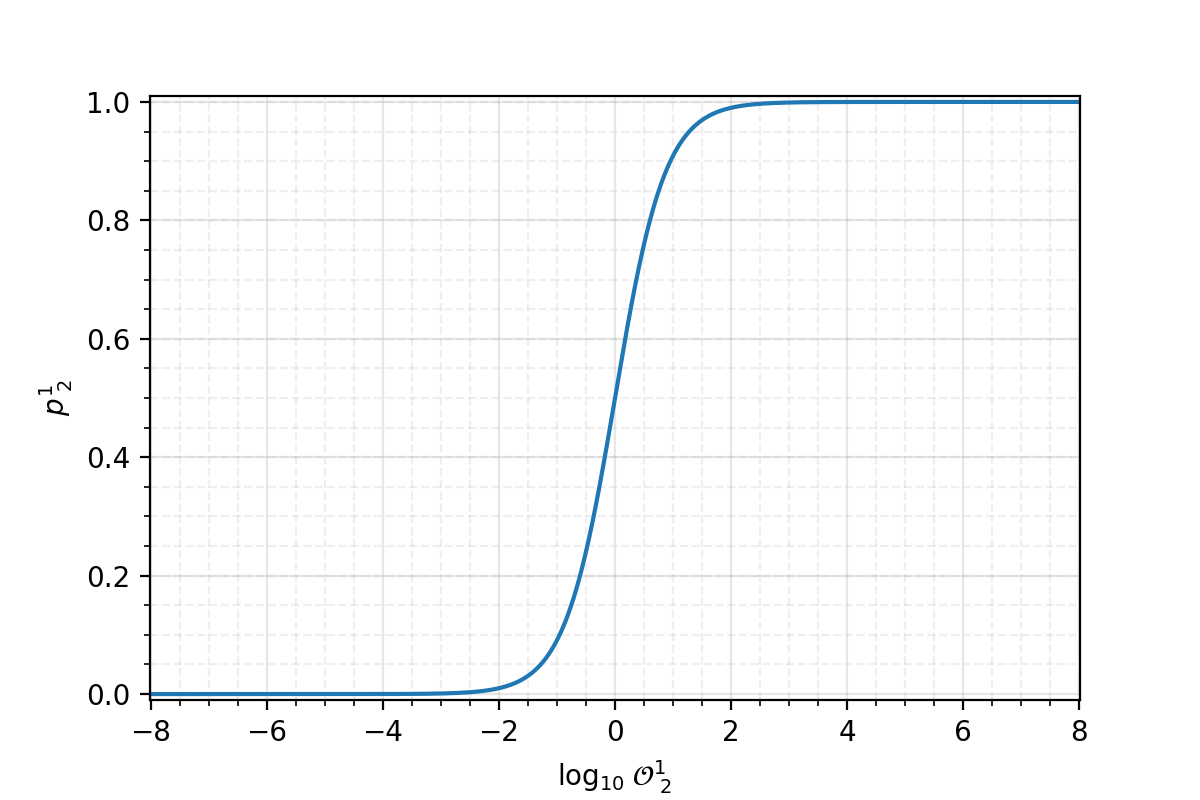
\includegraphics[width=\linewidth]{figs/chapter2/log10odds_probability.png}
  \caption{The probability of hypothesis 1 being favored over hypothesis 2 when considering the $\mathrm{log}_{10} \; \mathcal{O}$. When $\mathrm{log}_{10} \; \mathcal{O} = 0$, the probability for each hypothesis is $50\%$. At odds ratios close to 100 (0.01) the evidence becomes heavily stacked towards one hypothesis or another.}
  \label{fig:log10odds_v_probability}
\end{figure}
Furthermore, we can map this probability to a ranking statistic that is more familiar to Frequentists. That is the one-tailed z-score which states the integrated probability density from $-\infty$ to a particular multiple of the standard deviation of a Gaussian function. A z-score of $0 \sigma$ indicates a $50\%$ probability, while a z-score of $5 \sigma$ is $\sim$ $1-10^-7$ probability. We place a plot of this below for convenience.
\begin{figure}
  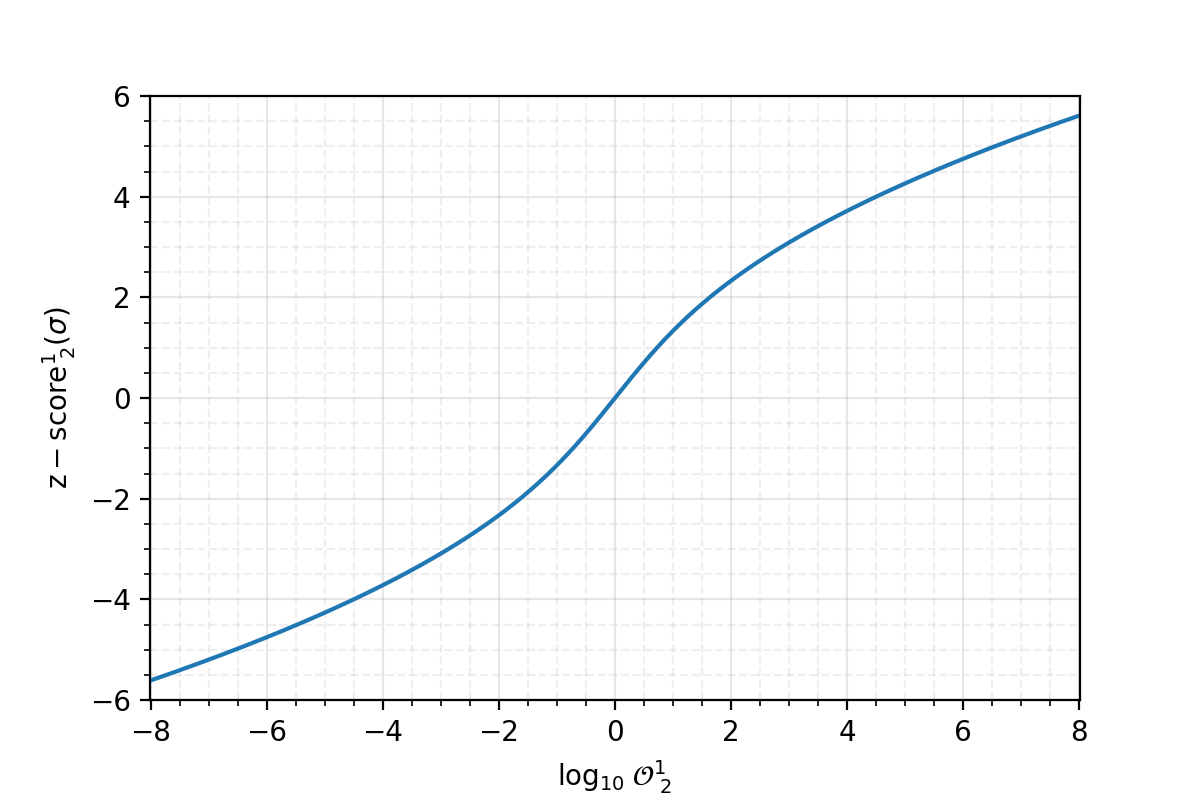
\includegraphics[width=\linewidth]{figs/chapter2/log10odds_z_score.png}
  \caption{The Frequentist z-score pertaining to the same level of probability for  hypothesis 1 being favored over hypothesis 2 when considering the $\mathrm{log}_{10} \; \mathcal{O}$. When $\mathrm{log}_{10} \; \mathcal{O} = 0$, the z-score is $0 \sigma$ and the probability for each hypothesis is $50\%$. A z-score of $>5 \sigma$ has the same probability value as an odds ratio of $> 10^7$.}
  \label{fig:log10odds_v_z_score}
\end{figure}

One convenient property of odds ratios is that we can stack evidence from multiple events if we continue to measure new data with our same prior hypotheses. In this manner, it is possible to take low significant results from multiple experiments and gradually build evidence for a hypothesis over many experiments. This requires that each experiment is a statistically independent event from the others, which is for all intents and purposes guaranteed in gravitational wave astronomy.

\subsubsection{Bayesian Model Averaging}

Bayesian statistics is based centrally around inferences from Bayes theorem. And as such there is no distinction necessary for inferences over parameters and inferences over models themselves. This provides a simple way to extend a singular analysis into an ongoing inference over multiple data sets or over multiple hypotheses. It provides a robust method for comparing and combining multiple inferences when data are informative or uninformative. As such we describe a methodology for combining the results of multiple hypothesis inferences called Bayesian model averaging as found in Kass and Raftery.

The concept of Bayesian model averaging is to average over many different models after evaluating the marginal likelihood for each model. In particular, one considers a fiducial standard model, $A$, of which the marginal likelihoood of $A$ will be compared to every other model. Thus for $N$ models we generate $N$ Bayes factors, where model $A$'s Bayes factor is simply unity since it is the fiducial standard model. In the case that all of the Bayes factors, $B_i$, are not definitive for one model or another, we must consider the possibility that since our parameters are conditioned on the model that we have elected, that we must seriously consider the effect of choice of model on various parameters. Given a sufficiently large set of models we can try to extract knowledge about the parameters that describe our data by marginalizing over many models. The formalism for this procedure follows immediately from Bayes theorem. Consider the following marginal posterior probability distribution for some model:
\begin{equation}
    \mathcal{P}(H_i|D) = \frac{\mathcal{B}^{H_i\;\;}_{\;\;H_A} \; \pi(H_i)}{\sum_{i=1}^N \mathcal{B}^{H_i\;\;}_{\;\;H_A} \; \pi(H_i)}.
\end{equation}
Here we have the posterior probability of some hypothesis given the data ... and the prior probability that we had for each model $H_i$...
Next, we consider a parameter $x$ that is present in all models thus considered such that our marginal posterior probability on $x$ given all of the models can become:
\begin{equation}
    \mathcal{P}(x|D) = \sum_{i=1}^N \mathcal{P}(x| D, H_i) \; \mathcal{P}(H_i|D).
\end{equation}
Here $\mathcal{P}(x| D, H_i)$ represents the marginal posterior probability distribution of $x$ under a particular hypothesis $H_i$, and so we coherently combine our inferences from multiple models by marginalizing over models. While, in practice there are an infinite number of models from which to draw inference on, there are usually only a finite set of probable models that we desire to investigate. All other models we can set our prior probabilities $\pi(H_i)$ to $0$, or sufficiently close to $0$ that they do not contribute to the analysis.

In the face of model uncertainty with respect to a particular data set, this provides us a consistent method for combining the results of multiple models in a self-consistent manner.

\subsubsection{Multiple Data Sets: Combining Evidence}
Multiplying through independent events...


Generally however, one must construct a model of models of sorts, a hyper-model that describes ...

\section{Frequentism and Bayesianism}
Above we have presented very brief outlines of different statistical frameworks which will be relevant to examining various hypotheses of gravitational wave analysis from aLIGO data. We have presented two statistical frameworks for examining hypotheses. The Frequentist interpretation is based on an interpretation of probability where if an outcome of some process is given a $70\%$ probability of occurring, this is to be interpreted that if the event is allowed to occur, under the same conditions, $100$ times, that we should expect the particular outcome to occur $70$ times. A Bayesian interpretation of probability is that we are trying to make a statement of our beliefs about how likely an outcome is to occur. Rather than probabilities describing the relative frequency that we can expect a particular result, probabilities encode our ignorance of the exact outcome of an event.

Both methods permit us to make rational inferences based on the measurements that we make in our data. Frequentist statistics has been a mainstay in gravitational wave astronomy for many years, but with the advent of advanced computational and numerical techniques, Bayesian statistics is seeing increasing use in gravitational wave astronomy.

While statistical inference give us some mathematical tools to better understand the correlations present in our data, they do not give us the full tools for making scientific decisions. The full expression of making a reasonable scientific inference relies in the experimental design and rational tools of investigation all the way through to conclusion. Statistics give us means to help justify some of these scientific choices but there is no statistical recourse for poor experimental design choices. It is always best to outline the research decisions made and try to account for plausible alternatives or future lines of investigation.


\Chapter{Introduction to Gravitational Wave Data Analysis}
\label{ch:GWData_Analysis}
uhmm?


\Chapter{Upper Limits on the Estimated Rate of Mergers of Systems with a Neutron Star}
\label{ch:BNS_NSBH_Upper_Limits}
The content of this chapter are primarily taken from ``Upper Limits on the Rates of Binary Neutron Star and Neutron-Star–Black-Hole Mergers from Advanced LIGO’S First Observing Run" in 2016. The main focus is on the results from the PyCBC offline search analysis conducted in this study.

Between September $12^\mathrm{th}$, $2015$ and January $19^\mathrm{th}$, $2016$, the two aLIGO detectors in Hanford, Washington and Livingston, Lousiana conducted their first observing period. During the first observing run two binary black hole coalescences were confidently observed by the offline PyCBC gravitational wave search pipeline with a p-value of being generated by noise of less than $10^{-7}$. A third candidate, termed LVT151012, was also observed by PyCBC, although with a smaller p-value. The masses of these binaries were assessed to not be compatible with the expected masses of neutron stars, and thus must be black hole binaries. This study assessed upper limits on the expected rate of mergers of neutron star binaries and neutron-star-black-hole binaries.

\section{The PyCBC Offline Search in the First Observing Run}
Below we briefly describe the methodology of the PyCBC Offline Search Pipeline in the first observing period.

The PyCBC Offline search analysis (cite) is a matched filter search for compact binary coalescence...

Derive matched-filter-snr...

\subsection{A Compact Binary Coalescence Template Bank}

The PyCBC Offline search is a modeled-search for gravitational waves from compact binary coalescence. And so we construct a bank of potential templates for astrophysical gravitational wave signals. This bank is referred to as the template bank and holds a catalog of gravitational wave signals that could be discovered. To do so we are required to generate templates in such a way as to span the parameter space of potential signals. In the first observing run, the template bank was a four-dimensional (parameter) bank. The four parameters were component masses of the binaries, $m_1$, $m_2$, and the component angular-momentum aligned-spin of the binary $\chi^z_1$ and $\chi^z_2$. The masses are drawn such that $m_1 > m_2$, which helps reduce the size of the template bank. The aligned-spin components are drawn to reflect the expected astrophysical properties of the binaries in that respective region of the mass parameter space.

The template bank is segmented into three sections, intended to find BNS, NSBH, and BBH signals. 
The template bnak in the first observing run consisted of approximately $250,000$ templates.

For $n$ detectors the harmonic mean of the detector's power spectral densities is chosen as the reference power spectral density when designing a common template bank for the Hanford and Livingston detectors. Previous searches used independent template banks for independent detectors, however this was not done in the first-observing run.

As the run progresses the template bank is validated using injected software signals to ensure that the noise properties of the detector have not changed to a sufficient degree as to make the template bank and template placement ineffectual in recovering expected signals. To do so, a population of simulated signals are expected to have a minimal match of $97 \%$ with any particular template in the bank. This is often called the Fitting Factor of the template bank. It is often a desired trait that less than $1\%$ of the simulated signals exhibit less than a $3 \%$ loss in anticipated signal-to-noise-ratio due to the discreteness of the template bank (or the change in the detector's power spectral density). The template bank was validated several times across the entire first observing run and only one template bank was necessary for the duration of the analysis.

\subsection{Data Quality and Conditioning}
It is well-known in the gravitational wave community that the output of the detector is not Gaussian and non-stationary over long periods of times and that the quality of the data from the interferometers is not always suitable for gravitational-wave analysis (cite). For this reason, the data undergo data quality checks and data conditioning prior to being analyzed for gravitational wave events.

In particular, there are several data quality vetoes

Gating

\subsection{The Ranking Statistic: Signal-to-Noise-Ratio and NewSNR}
Derive SNR from Gaussian distribution

Maximize over amplitude

Maximize over phase

However, the noise in the detector is decidedly not Gaussian, nor stationary and so the a new ranking statistic was developed as a further signal consistency check. The signal-to-noise-ratio statistic was made subject to a reduced $\chi^2$ consistency check, hence labeled as $\chi_r^2$. The $\chi_r^2$ test separates the signal into $k$ frequency bins and measures the accumulated signal-to-noise-ratio in each frequency bin. For a true signal, we expect a steady contribution to the signal-to-noise-ratio from each frequency bin. Thus, the $\chi_r^2$ test for a true signal embedded in Gaussian noise returns a value $\leq 1$, while a $\chi_r^2$ value $>1$ indicates a poor fit to the data across all frequency bins. The $\chi_r^2$ test can be expressed as:
\begin{equation}\label{eqn:reduced_chi_sq}
    \chi^2_r = \frac{k}{2k-2} \sum^k_{i=1} \left(\rho_i - \frac{\rho_i}{k}\right)^2
\end{equation}
Here $\rho_i$ represents the signal-to-noise-ratio in the $i^{\mathrm{th}}$ frequency bin, and $k$ is the number of frequency bins.

Prior to the first observing run, $k=16$ frequency bins were used, however, in the first observing run the number of frequency bins used was dependent on the peak frequency of the template. The formulation in the first observing run was, $k = 0.4\left[f_\mathrm{peak} / \mathrm{Hz}\right]^{2/3}$, and $k$ is rounded to the nearest integer. Next, the reduced $chi^2$ values are used to re-rank the signal-to-noise-ratio ranking statistic through an empirically designed ranking statistic called newSNR. When $\chi^2_r > 1$, newSNR can be calculated as:
\begin{equation}\label{eqn:newsnr}
    \hat{\rho} = \frac{\rho}
                  {\left\{\left[ 1 + \left(\chi^2_r\right)^3\right]/2\right\}^{1/6}}
\end{equation}
For values of $\chi^2_r \leq 1$, NewSNR is equal to the signal-to-noise-ratio ($\hat{\rho} = \rho$), while for values of $\chi^2_r >1$, Eq.~\ref{eqn:newsnr} is applied and newSNR is less than the signal-to-noise-ratio ($\hat{\rho}_c < \rho$). Finally then, for the Livingston and Hanford detectors the ranking statistic of a candidate trigger is $\hat{\rho}^2_\mathrm{network} = \hat{\rho}_\mathrm{L1}^2 + \hat{\rho}_\mathrm{H1}^2$. For a more detailed description of the first observing run's ranking statistics and the $\chi^2_r$ please consult N, N.

\subsection{Evaluation of the Statistical Significance of Events}
Description of timeslides

After coincident triggers are collected across five days of coincident analysis time between the two detectors. These coincident triggers are the foreground event triggers and are potentially of astrophysical origin. In order to assess the statistical significance of these foreground triggers we need an estimate of the rate at which non-astrophysical or background noise could potentially generate triggers of similar magnitude in the ranking statistic. Unfortunately, gravitational waves cannot be shielded from as electromagnetic waves can be, and so we use an empirical method to estimate the false alarm rate of triggers at a specific loudness in ranking statistic.

Description of inclusive and exclusive background

Description of p-value evaluation for single events

Since $n=3$ independent PyCBC offline searches were carried out in the first observing run for different compact binary coalescences, a Bonferroni correction is applied to the measured p-values from each search. The Bonferroni correction, or trials factor, states that if one conducts $n$ trials in searching for an effect, the threshold $\alpha$ on the p-value should also be divided by the number of trials $n$. This provides a conservative method for re-ranking the statistical significance of events provided multiple instances of searches. Since the different CBC search categories are weakly correlated (e.g. GW150914 was seen in the BBH search and the BBH-NSBH search), a better p-value correction could be considered to be less than $3$. Quantifying this level of correlation however, was beyond the scope of the study.

The p-value of a particular event can then be converted to a z-score, or the number of standard deviations in a one-tailed Gaussian probability integral via: 
\begin{equation}
    z = - \sqrt{2} \, \mathrm{erf}^{-1} \left[1 -  2 \left(1-\, p\right)\right].
\end{equation}
Here $z$ represents the z-score, $\mathrm{erf}^{-1}$ is the inverse error function, and $p$ is shorthand for the p-value (e.g. $0.05$). It is standard practice in many subfields of physics to require a z-score of $5$ (sometimes called $5 \sigma$) level of confidence before rejecting the null hypothesis that noise generated the gravitational wave signals. This corresponds to a p-value of $< 10^{-7}$.

Additional data quality checks are then used to verify that the gravitational wave candidate is more consistent with a signal hypothesis than with the null (noise) hypothesis. The probability that the event is of astrophysical origin cannot be gathered from the p-value itself but requires the use of Bayes Rule to calculate the probability of being of astrophysical origin, $p_\mathrm{astro}$. P-values are statements about the probability of observing data greater than some critical value under the assumption that the null hypothesis is true, while the probability of the event being astrophysical is a probability of a hypothesis being true (that the signal model better \textit{explains} the candidate than a noise model).

\subsection{Results of the Search}


The PyCBC offline search analysis found two confident gravitational wave events, GW150914 and GW151226, with statistical significance $> 5 \sigma$ (p-value $<  10^{-7}$) and a gravitational wave candidate, LVT151012, with a statistical significance of $\sim 2\sigma$. These statistical significance values are quoted after a trials factor of $3$ was applied to the analysis. All three triggers were found to be consistent with stellar mass black hole binaries, although LVT151012 was not confidently claimed as a detection.

No statistically significant BNS or NSBH events were found. And so we turn towards trying to determine an upper limit on the rate of mergers of BNS and NSBH events.

\section{Bayesian Rates Estimation}
Since no events were discovered in the first observing run, we seek to try to model the expected number of events for BNS and NSBH events. The expected number of events $\Lambda$ can be expressed as:
\begin{equation}
    \Lambda = R \, \langle VT\rangle.
\end{equation}
Here, the rate of mergers is given by $R$, and $\langle VT\rangle$ describes the sensitive-spacetime volume averaged over space, observation time, and the parameters of the source population of interest. The units of a rate are henceforth in $\mathrm{Gpc}^{-3} \mathrm{yr}^{-1}$. For reference the core-collapse supernova rate is $\sim 10^5 \, \mathrm{Gpc}^{-3} \, \mathrm{yr}^{-1}$ (Cappellaro et al. 2015).

Here we assume that gravitational wave events are exceedingly rare, and so we can model the likelihood for finding an observation of a gravitational wave event in the data $D$ as a Poisson distribution. The likelihood of seeing $s_i$ independent events after $N$ observations, given some $\Lambda$ can be expressed as:
\begin{equation}\label{eqn:poisson_likelihood}
    p\left(s|\Lambda\right) = \prod_{i=1}^N \frac{1}{s_i!}\Lambda^{s_i} e^{-\Lambda}
\end{equation}
In the case that we have zero observations, in one observing period, this likelihood can be written as:
\begin{equation}\label{eqn:no_event_poiss_like}
    p\left(s|\Lambda\right) = e^{-\Lambda}.
\end{equation}
Using Bayes theorem we can find a posterior probability on the number of expected rates as:
\begin{equation}\label{eqn:posterior_lambda_simple}
    p\left(\Lambda|s\right) \propto p\left(\Lambda\right) p\left(s|\Lambda\right).
\end{equation}
Here $p\left(\Lambda\right)$ is our prior belief on $\Lambda$, the number of expected mergers. The most straightforward prior distribution to use is a conjugate prior distribution. The advantage of a conjugate prior distribution is that our posterior distribution will be of the same kind or type of distribution as the prior distribution. For a Poisson likelihood the conjugate prior is proportional to a Gamma probability distribution, in our case we express this as:
\begin{equation}\label{eqn:prior_lambda_simple}
    p\left(\Lambda\right) \propto \Lambda^{\alpha}.
\end{equation}
A conjugate prior when multiplied with its respective likelihood distribution gives a posterior distribution that is within the same family of functions as the prior distribution. Setting $\alpha=0$ gives a uniform prior distribution, while setting $\alpha = 1/2$ gives $p\left(\Lambda\right) \propto 1/\sqrt{\Lambda}$. This is the Jeffreys prior for the Poisson likelihood in that it is an uninformative prior. A Jeffreys prior is sometimes useful in that it gives a equal prior probability weight to all possible values of the parametrization of the Bayesian inference.

Prior information from previous LIGO data were not used in a prior on $\Lambda$ due to changes in the detector sensitivity and the large changes to $\langle VT\rangle$.

The likelihood $e^{-\Lambda}$ is estimated by empirically measuring $\langle VT\rangle$ through the use of software injections of gravitational wave events into the aLIGO data set. These software injections involve generating gravitational wave strain data for different astrophysical objects in the radiation frame and then projecting them into the detector frame. These simulated signals are then added in to aLIGO data for detection.

Simulated signals are considered to be recovered when they are detected with an IFAR of $> \, 100 \, yrs$.  Since only a finite set of software injections can be processed and recovered, we use Monte-Carlo integration techniques to estimate the volume of injections recovered and a variance estimate of the volume recovered. The volume of injections recovered is compared then to the spacetime volume that the injections were injected from. Furthermore, the uncertainty in the calibration of the detector plays a role in the uncertainty in the recovered volume, since the calibration of the data plays a role in recovered signal-to-noise-ratios of simulated signals. It was found that the calibration added an $18 \%$ uncertainty to the estimated sensitive volume $\langle VT \rangle$. There is an additional uncertainty due to waveform modelling between injected simulated signals and waveform models used for recovery. This is additionally folded into the uncertainty on $\langle VT \rangle$.

It is convenient to consider the posterior on $\Lambda$ as a joint-posterior on the variables that compose $\Lambda$, that being $R$ and $VT$. To do so we can refactor the prior distribution on $\Lambda$ into a joint prior distribution on $R$ and $\langle VT \rangle$.
\begin{equation}\label{eqn:joint_posterior_simple}
    p\left(R, \langle VT \rangle \right) = p\left(R | \langle VT \rangle\right) \, p\left( \langle VT \rangle \right).
\end{equation}
In this publication, the prior $p\left(R | \langle VT \rangle\right)$ was chosen to be uniform in $R$, or a Jeffreys prior given by, $1/\sqrt{R \langle VT \rangle}$. In keeping with previous Refs, (Abbott et al. 2016f,m,c), the prior distribution on $\langle VT \rangle$ is given as a log-normal distribution given by:
\begin{equation}\label{eqn:prior_vt}
    p\left(\langle VT \rangle \right) =
            ln \, \mathcal{N} \left( \mu, \sigma^2\right).
\end{equation}
Here $\mu$ is the average value for $\langle VT \rangle$ obtained from the offline search, and $\sigma$ represents the $18 \%$ uncertainty in $\langle VT \rangle$ due to calibration uncertainty.

Thus the posterior of $\Lambda$ in the new parametrization becomes:
\begin{equation}\label{eqn:posterior_lambda}
    p \left(R, \langle VT \rangle \right) \propto p\left(R, \langle VT \rangle \right) \, e^{-R \langle VT \rangle}.
\end{equation}
To obtain a posterior distribution on the rate $R$ of mergers of a certain class we are required to marginalize the joint-posterior in $R$ and $\langle VT \rangle$ over $\langle VT \rangle$. This can be expressed as:
\begin{equation}\label{eqn:posterior_rate}
    p\left(R | s\right) = \int p \left(R, \langle VT \rangle | s \right) d\langle VT \rangle.
\end{equation}
Finally then, the upper limit on the rate at the $90 \%$ credible level is possible by integrating the marginalized posterior distribution of $R$ from $0$ to an upper-value of $R_\mathrm{critical}$ that grants a $90 \%$ probability.
\begin{equation}\label{eqn:90perc_conf_int}
    0.9 = \int_0^{R_{\mathrm{critical}}} p\left(R | s\right) dR.
\end{equation}
For a uniform prior in $p \left(R, \langle VT \rangle | s \right)$ and no uncertainty in $\langle VT \rangle$ the $90 \%$ credible limit is given as:
\begin{equation}\label{eqn:freq_90_perc}
    R_{\mathrm{critical}} = \frac{- ln \left( 1 - 0.9 \right)}{\langle VT \rangle} = \frac{2.303}{\langle VT \rangle}.
\end{equation}
The expression in Eq.~\ref{eqn:freq_90_perc} is also the Frequentist's $90 \%$ confidence interval(cite Jolien), although one should be careful in that the interpretation of the intervals are distinct in Frequentism and Bayesianism. Under the Jeffreys prior on $p \left(R, \langle VT \rangle | s \right)$ the upper limit can be expressed as:
\begin{equation}\label{eqn:jeffreys_90_perc}
    R_{\mathrm{critical}} = \frac{\left[\mathrm{erf}^{-1}\left(0.9 \right) \right]^2}{\langle VT \rangle} = \frac{1.353}{\langle VT \rangle}.
\end{equation}

Using these expressions, we can thus model the rate of mergers $R$ of a particular class of binaries by conducting software injections for that class of binaries that model our expectations of the astrophysical population for that binary.

\subsection{Astrophysical Populations of BNS and NSBH}
There are thousands of identified neutron stars, of which the majority are detected as pulsars (). Of these there are an estimated 70 neutron stars identified as binary neutron stars. Mass estimates of neutron stars range between $\approx \, 1 M_\odot$ to $3 M_\odot$. Eight candidate neutron star binaries permitted measurement of the binary component masses (), of which an estimate of the distribution of events is consistent with $\mathcal{N} \left(\mu = 1.35, \sigma^2 = 0.13^2 \right)$.

With respect to the spin characteristics of neutron stars, the fastest spinning pulsar was measured to have a rotational frequency of $716 \, Hz$. For reasonable estimates of the mass and moment of inertia for this pulsar, this corresponds to a dimensionless spin $\chi = c |S| / (G m^2) \sim 0.4$, where $m$ is the mass of the pulsar, $c$ is the speed of light, $G$ is Newton's gravitational constant, and $|S|$ is the angular momentum. However, the fastest spinning neutron star in a binary system is estimated to have a $\chi \leq 0.04$ (Brown et al). A neutron star in a binary can be spun up to larger rotational frequencies if its binary companion accretes matter and angular momentum on to the neutron star. This is called a recycled neutron star and estimates of the spin of a possible candidate BNS pulsar J1807-2500B is $\chi \sim 0.2$.

With these things in mind, our simulated astrophysical population for neutron star binaries contains two distinct populations in the mass parameters that we simulate. The first BNS population is drawn uniform in component masses between $\left[1, 3\right] M_\odot$, while another population is drawn with mass distribution, $\mathcal{N} \left(\mu = 1.35, \sigma^2 = 0.13^2 \right)$. Each mass distribution is also subject to two distinct component spin distributions. The first spin distribution is an isotropic component-spin distribution such that $|\chi_i| < 0.05$. The second spin distribution is an isotropic component-spin distribution with $|\chi| < 0.4$. This second spin distribution is drawn with considerations from (Nitz 2015) that it is not necessary to create a template bank modeling the spin distribution of BNS mergers above $0.4$ since BNS mergers with spin $> 0.4$ can still be well recovered by templates with $\chi_i < 0.4$.

Neutron-star-black-hole systems are thought to be efficiently formed in one of two ways: either through the stellar evolution of field binaries or through dynamical capture of a NS by a BH (Grindlay et al. 2006; Sadowski et al. 2008; Lee et al. 2010; Benacquista and Downing 2013). Though no NSBH systems are known to exist, one likely progenitor has been observed, Cyg X-3 (Belczynski et al. 2013).

NSBH mass distribution

NSBH spin distribution

Each population is also simulated according to a uniform distribution in the binary orientation, that is to say that no binary orientation relative to the detector is preferred. This means that binaries are drawn from a probability distribution that is uniform in $\iota$, inclination angle, and $\Psi$ polarization angle. The binaries are also distributed uniformly across the sky, which is uniform in $\alpha$ right ascension and $\delta$ declination.

Finally, binaries are drawn uniformly in comoving volume, which we briefly describe below following (Hogg 1999). A comoving volume in terms of cosmology means the volume of the universe assuming a frame of reference which expands with the universe. In particular we measure a comoving volume out to a particular luminosity distance or redshift $z$. The redshift $z$ is defined via:
\begin{equation}
    1 + z = \frac{a(t_o)}{a(t_e)}.
\end{equation}
The redshift $z$ is defined via the ratio of $a(t_0)$, the size of the universe (scale factor) at the time of observation, and $a(t_e)$, the size of the universe at the time of emission. As the name implies the redshift factor relates how light (or gravitational waves) are redshifted in frequency due to the expansion of the universe. Those who are interested in the explicit definition of comoving volume can see (Hogg 1999) as the formal definition in terms of measured and inferred cosmological constants is quite involved. The comoving volume is dependent on $H_0$, $\Omega_M$, $\Omega_\Lambda$ and $\Omega_k$ measured or inferred values from Planck2015.

Here $H_0$ is the Hubble constant which relates the present-time recessional velocity of distant stars relative to the distance of the distant stars in the form $v = H_0 d$. The Hubble constants is measured in experiment. We have the term $\Omega_M \equiv \frac{8 \pi G \rho_0}{3 H_0^2}$, where $G$ is Newton's gravitational constant and $\rho_0$ represents the measured mass density of the universe at the present time. We also have the term $\Omega_\Lambda \equiv \frac{\Lambda c^2}{3 H_0^2}$, where $\Lambda$ is the cosmological constant representing the energy density of space, and $c$ is the speed of light. Finally then $\Omega_k \equiv 1 - \Omega_\Lambda - \Omega_M$, defining a homogeneous, isotropic, and matter dominated universe, and is responsible for describing the spacetime curvature of the universe. We take the mean values from  Planck2015 without any associated variation on the parameters.

Due to cosmological distances being involved the masses of binaries will be measured in the detector frame, $M_\mathrm{det}$, relative to the source frame mass, $M_\mathrm{src}$ under the relation:
\begin{equation}
    M_\mathrm{det} = \left(1 + z \right) M_\mathrm{src}
\end{equation}

%# From Planck2015, Table IV
%# https://arxiv.org/pdf/1502.01589.pdf
%# See /home/steven.reyes/pycbc-dev-lalinference-o1-032616/src/lalsuite/lalsuite/lal/src/tools/LALCosmologyCalculator.c
%# https://lscsoft.docs.ligo.org/lalsuite/lal/_l_a_l_cosmology_calculator_8c_source.html
%omega = lal.CreateCosmologicalParametersAndRate().omega
%lal.SetCosmologicalParametersDefaultValue(omega)
%omega.h = 0.679 # 67.90 ± 0.55 Hubble constant H0 TT+lowP+lensing+ext 68 % limits
%omega.om = 0.3156 # Omega M 0.3156 ± 0.0091 TT,TE,EE+lowP 68 % limit
%omega.ol = 0.6935 # Omega Lambda 0.6935 ± 0.0072 TT+lowP+lensing+ext 68 % limit
%omega.ok = 1.0 - omega.om - omega.ol # this is an equation if the universe is homogeneous, isotropic, and matter dominated
%omega.w0 = -1.0
%omega.w1 = 0.0
%omega.w2 = 0.0

Waveform models used
BNS TaylorT4
NSBH 

The software injections are generated in the radiation frame using time domain waveforms. They are assigned a geocentric time of arrival (coalescence) at which point they are projected from the radiation frame onto a specific detector frame for the Livingston and Hanford detectors respectively. This strain is then added into the strain of the data at the time of arrival. 

\subsection{Rates Inference Results}
Using the equations in the previous section we found improved upper limit results on the expected rate of mergers of BNSs and NSBHs.

The posterior probability density on the rate of merger of BNSs for a Gaussian-like distribution of masses can be found in Fig.~\ref{fig:bns_upper_limits} for the two different prior distribution choices on the rate of mergers. Following a uniform prior on $\Lambda$ we found that the $90\%$ credible level on the upper limit on BNS merger rate is $\sim 1.2 \times 10^4 \, Gpc^{−3} \, yr^{−1}$ for low-spin and high-spin populations. This is approximately a factor of $10$ improvement over (Abedie et al. 2012a). The posterior rates inference for a uniform mass distribution can be found in Fig.~\ref{fig:bns_uniform_upper_limits} and does not differ significantly from the inference results presented in Fig.~\ref{fig:bns_upper_limits}.

\begin{figure}
  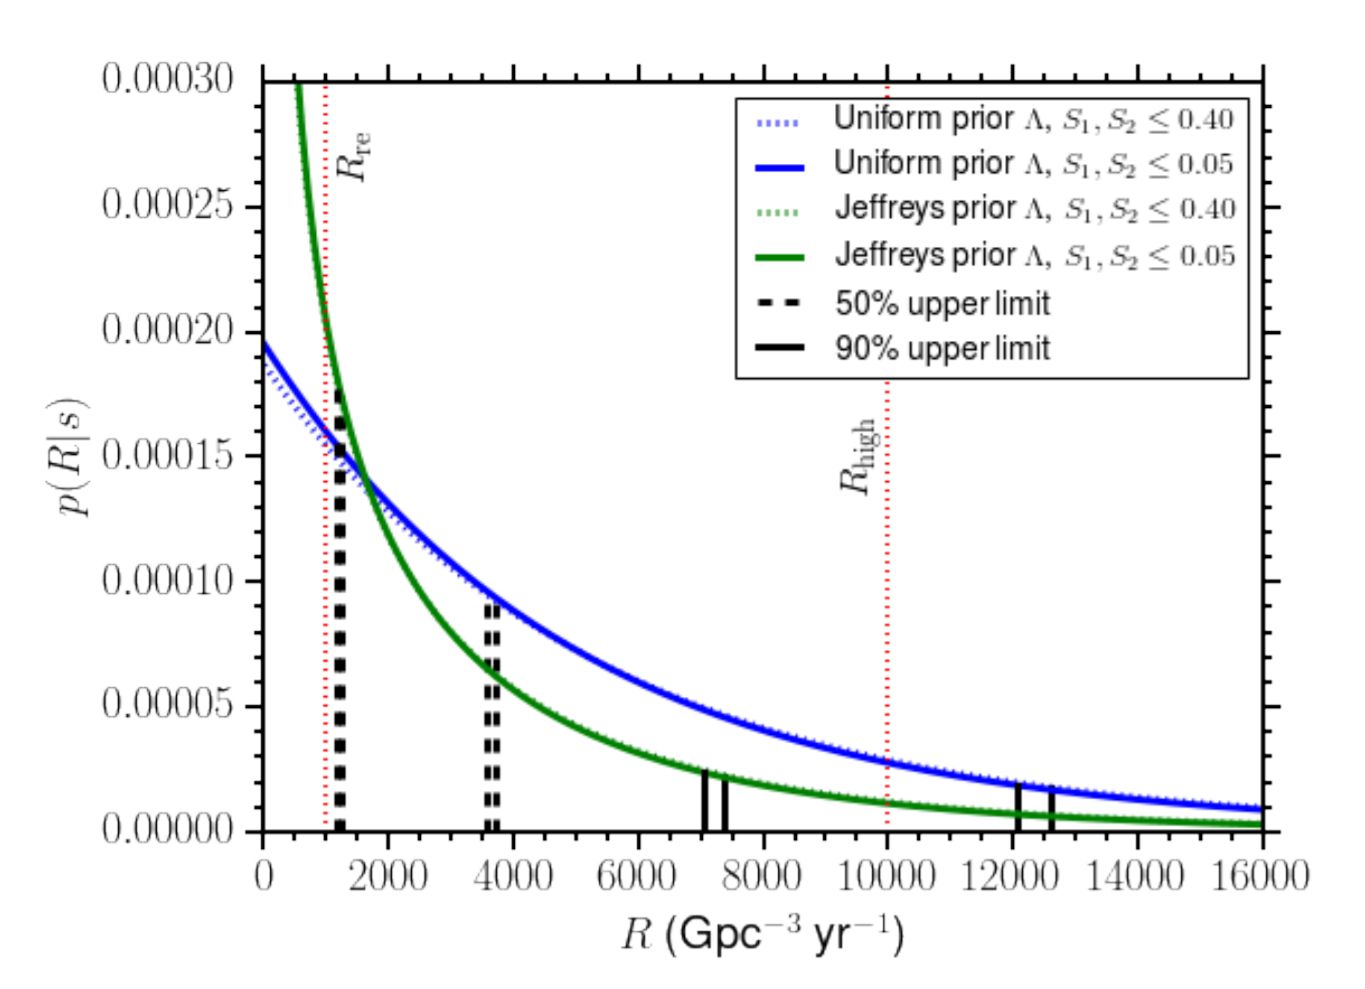
\includegraphics[width=\columnwidth]{figs/chapter4/bns_upper_limits_posterior_rates.png}
  \caption{Posterior probability density on the rate of BNS mergers. Blue curves represent a uniform prior on $\Lambda$, while green curves represent a Jeffreys prior on $\Lambda$. The solid (low spin population) and dotted (high spin population) posteriors almost overlap. The vertical dashed and solid lines represent the $50\%$ and $90\%$ credible upper limits respectively for each choice of prior on $\Lambda$. For each pair of vertical lines, the left line is the upper limit for the low spin population and the right line is the upper limit for the high spin population. Also
  shown are the realistic $R_\mathrm{re}$ and high end $R_\mathrm{high}$ of the expected BNS merger rates identified in Ref. (Abadie et al. 2010).}
  \label{fig:bns_upper_limits}
\end{figure}

\begin{figure}
    \centering
    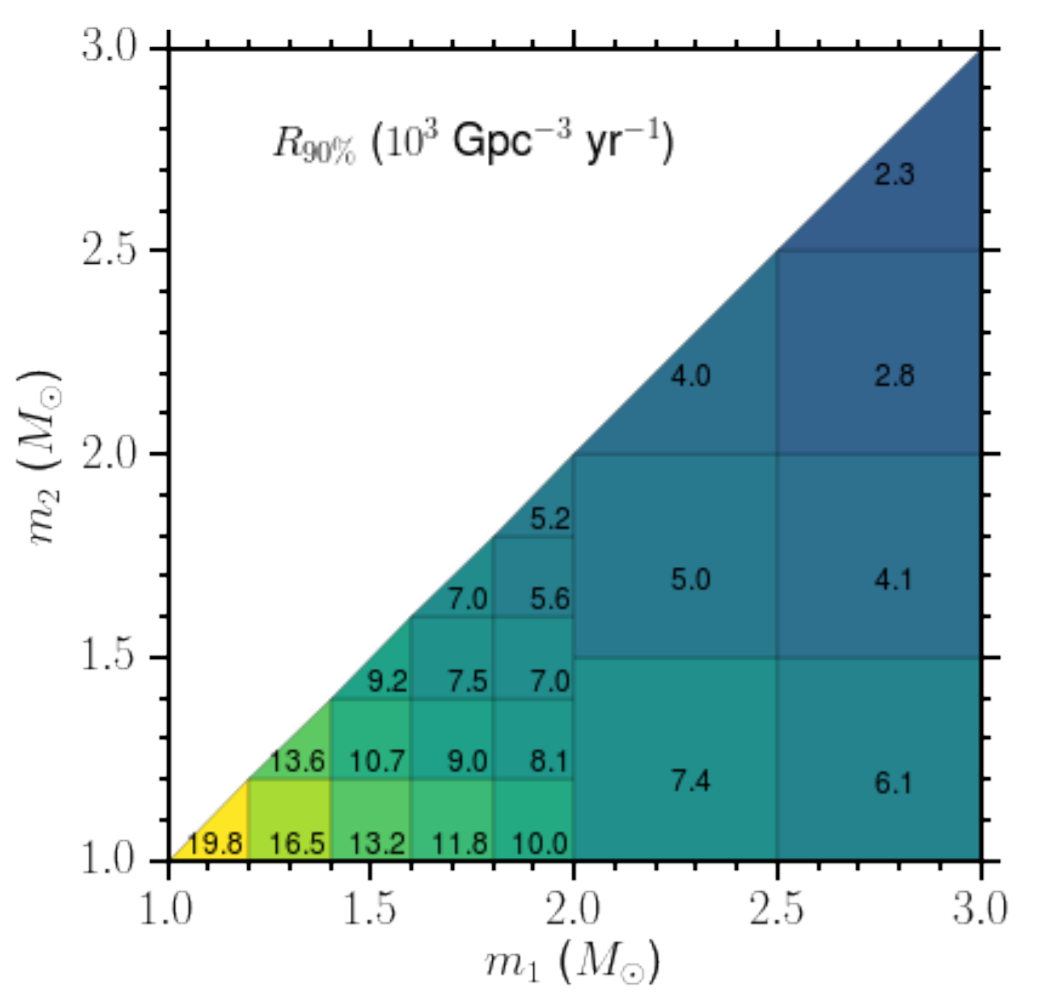
\includegraphics[width=\columnwidth]{figs/chapter4/bns_uniform_mass_isotropic_low_spin_rates.png}
    \caption{The $90 \%$ credible upper limit on the BNS merger rate as a function of the two component masses. Here the upper limit for each bin is obtained assuming a BNS population with masses distributed uniformly within the limits of each bin, considering isotropic spin direction and dimensionless spin magnitudes uniformly distributed in $[0,0.05]$.}
    \label{fig:bns_uniform_upper_limits}
\end{figure}

The $90 \%$ posterior probabilty upper limits on the rate of mergers for NSBHs can be summarized in Table~\ref{tbl:nsbh_posteriors}. We found that the search is less sensitive to populations of NSBHs with isotropic spin distributions when compared to (anti-) aligned spin distributions. One factor that contributes to this increased sensitivity to (anti-) aligned spin NSBHs is the fact that the template bank is constructed using (anti-) aligned spin templates and not isotropic-spin distributed templates.

\begin{table}[h!]\label{tbl:nsbh_posteriors}
\centering{}
 \begin{tabular}{||c c c c ||}
 \hline
 NS Mass ($M_\odot$) & BH Mass ($M_\odot$) &  Spin Distribution & $R_{90 \%}$ \, ($Gpc^{-3} \, yr^{-1}$) \\
 \hline\hline
 1.4 & 5 & Isotropic & 3,600 \\ 
 \hline
 1.4 & 5 & Aligned & 3,210 \\
 \hline
 1.4 & 10 & Isotropic & 2,530 \\
 \hline
 1.4 & 10 & Aligned & 1,850 \\
 \hline
 1.4 & 15 & Isotropic & 2,300 \\
 \hline
 1.4 & 15 & Aligned & 1,280 \\
 \hline
\end{tabular}
\caption{The $90\%$ credible upper limit for NSBH systems with isotropic and aligned  spin distributions. The NS spin magnitudes are in the range [0,0.04] and the BH spin magnitudes are in the range [0,1].}
\end{table}


\section{Astrophysical Interpretation and Future Results}
The inferred upper limit estimation on the rate of binary mergers for compact binary mergers involving neutron stars permit us to explore if any population models for the genesis of these binaries can be ruled out by the available data. For BNS populations we compare our posterior rate estimations with $10$ other studies. While for the NSBH populations we compare our posterior rate estimations with $9$ other studies.

For BNS populations we consider the population models from : During the first observing run our upper limit estimations on the rate of BNS mergers were not in conflict with any of the population models considered. It was estimated that assuming estimates of O2 and O3 aLIGO detector sensitivities that continued non-detections of BNS mergers in aLIGO's  second observing run and third observing run that our upper limits could begin to rule out some of the population models considered. Fortunately, however GW170817, a BNS merger event, was discovered in the second observing run.

For NSBH poppulations we consider the population models from:



BNS and NSBH mergers are considered to be possible sources for short-hard gamma ray bursts (). We can also explore a geometrical argument regarding the beaming angle of binary neutron stars and neutron star-black hole binaries if they are assumed to be the progenitors of short-hard gamma ray burst events.

Rate Implications on population Models

Explain short-hard gamma ray bursts...
Assuming that every merger from a BNS or an NSBH produces a gamma ray burst the rate of short-hard gamma ray bursts detected follows from a geometric relationship of the beaming angle of the gamma ray burst jet and the expected rate of mergers of these binaries. The relation can be given as follows:
\begin{equation}\label{eqn:grb_jet_angle}
    R_\mathrm{GRB} = \left[ 1 - cos \left(\theta_\mathrm{jet}\right) \right] R_\mathrm{merger}.
\end{equation}
The relation can be understood as an axially symmetric jet whose solid angle covers a fraction of a unit sphere that envelops the binary. Hence, for some rate of binary mergers, $R_\mathrm{merger}$, a fraction of these mergers will be seen as gamma ray bursts from which we can infer a rate of gamma ray bursts, $R_\mathrm{GRB}$. This fraction is related to the opening angle of the gamma ray jet, $\theta_\mathrm{jet}$. In blank we assumed a rate of gamma ray bursts of $R_{\mathrm{GRB}} = 10^{+20}_{-7} \mathrm{Gpc}^{-3} \mathrm{yr}^{-1}$ from (Nakar et al. 2006; Coward et al. 2012). The inferred beaming angles can then be constructed by using the estimates on $R_\mathrm{merger}$ from this study. The study found that we could infer at $90\%$ confidence that the gamma-ray burst jet angle must be greater than $2.\!\!^\circ3_{-1.1}^{1.7}$ if short-hard gamma ray bursts are exclusively caused by BNS mergers and if each BNS merger produces a short-hard gamma ray burst. This inference comes from the low-spin, Gaussian mass distribution population of BNS. If NSBH mergers from $5 M_\odot$ and $1.4 M_\odot$ with aligned spin distributions are considered as the main progenitors of short-hard gamma ray bursts then the 90$\%$ confidence interval is $\theta^{\mathrm{lower \, limit}}_\mathrm{jet} = 4.\!\!^\circ3_{-1.9}^{+3.1}$.

\subsection{GWTC-1: Inferences from the $1^{\mathrm{st}}$ and $2^{\mathrm{nd}}$ Observing Run}
The LIGO Scientific Collaboration and Virgo Collaboration (LVC) found in [] that from the confident BNS merger, GW170817, that they were able to place a posterior estimate on the rate of BNS mergers in the universe to be, at the $90\%$ credible interval to be between $110 - 3840 \, \mathrm{Gpc}^{-3}\mathrm{yr}^{-1}$, and with no confident NSBH merger detections a $90\%$ confidence upper limit on the rate of NSBH mergers of $610 \, \mathrm{Gpc}^{-3}\mathrm{yr}^{-1}$. Note that the $90^\mathrm{th}$ percentile matches relatively closely with the $50^\mathrm{th}$ percentile estimate for the uniform prior distribution on $\Lambda$ in Fig.~\ref{fig:bns_upper_limits}. The procedure for generating an upper limit on the rates given a detection event is somewhat different from the procedure outlined in this chapter, however the procedure in [] for estimating the upper limit on the rate of NSBH mergers is mostly identical to the procedure outlined in this chapter, with the exception of some changes to the PyCBC offline search pipeline in terms of ranking statistic of candidate triggers.


\Chapter{1-OGC}
\label{ch:1_OGC}
\newcommand{\note}[1]{{\color{red} [#1]}}
\def\cn{\note{cite}}

\newcommand{\chieff}{\ensuremath{\chi_{\mathrm{eff}}}}
\newcommand{\rankingstat}{\ensuremath{\tilde{\rho}_c}}
\newcommand{\tdr}{\ensuremath{\mathrm{TDR}}}
\newcommand{\far}{\ensuremath{\mathcal{F}}}
\newcommand{\tar}{\ensuremath{\mathcal{T}}}
\newcommand{\msun}{\ensuremath{\mathrm{M}_{\odot}}}
\newcommand{\pastro}{\ensuremath{P_{\mathrm{astro}}}}
\newcommand{\release}{\texttt{\url{www.github.com/gwastro/1-ogc}}}

\section{Introduction}
\label{sec:intro}
The following is taken from PAPER


The Advanced LIGO gravitational wave observatories~\citep{Martynov:2016fzi} performed their first observing run (O1) from September 12, 2015 to January 19, 2016. This provided a total of 51.5 days of coincident observations from the two detectors located in Hanford, WA and Livingston, LA. The binary black hole mergers observed in this observing run have been  reported by the LIGO and Virgo Collaborations (LVC) in \cite{Abbott:2016blz,Abbott:2016nmj,TheLIGOScientific:2016pea}.  These binary black hole detections have been independently studied by \cite{Green:2017voq,Roulet:2018jbe,Antelis:2018smo}.

Since the publication of the results by \cite{TheLIGOScientific:2016pea,Abbott:2016ymx}, improvements to the data-analysis methods used~\citep{TheLIGOScientific:2016qqj} have been implemented \citep{Nitz:2017svb,Nitz:2017lco,DalCanton:2017ala}.  Using these improvements, we re-analyze the O1 data and provide---for the first time---a full catalog of candidate events from a matched filter search for compact binary coalescences using the O1 data, which we call 1-OGC. This catalog provides estimates of the significance of previously known events and a ranked list of sub-threshold candidates. Although not significant by themselves, these sub-threshold candidates can be correlated with archival data or transient events found by other astronomical observatories to provide constraints on the population of compact-object mergers \citep{Ashton:2017ykh, Burns:2018pcl}.

Our catalog is based entirely on public, open data and software. We use the LIGO data available from the Gravitational Wave Open Science Center~\citep{Vallisneri:2014vxa}, and analyze the data using the open source PyCBC toolkit~\citep{Usman:2015kfa,Canton:2014ena,pycbc-github}.This toolkit was also used by one of the two analyses described in~\cite{TheLIGOScientific:2016qqj}. The lowest mass sources targeted in our search are neutron star binaries with total mass $m_1 + m_2 = 2\, M_\odot$. The search space extends to binary black hole systems that produce gravitational waveforms longer than $0.15$~s from $20$~Hz. This corresponds to a total mass up to $500 M_{\odot}$ for sources with high mass ratios and spins where the component aligned with the orbital angular momentum is positive and large. For binaries with negligible spin, this corresponds to total mass $\lesssim 200 M_{\odot}$. The search space also includes neutron star--black hole binaries. After applying cuts for data quality~\citep{TheLIGOScientific:2016zmo,TheLIGOScientific:2017lwt}, a total of 48.1~days of coincident data are searched for signals.

The three most significant signals in the catalog correspond to GW150914~\citep{Abbott:2016blz}, LVT151012~\citep{Abbott:2016blz,TheLIGOScientific:2016pea}, and GW151226~\citep{Abbott:2016nmj}, respectively. No other astrophysically significant signals are observed. In the analysis of \cite{TheLIGOScientific:2016pea}, LVT151012 was the third-most significant event, but it was not sufficiently significant to be labeled as an unambiguous detection. With the improved methods employed here, the false alarm rate of this candidate improves by an order of magnitude and it should be considered a true astrophysical event. The analyses of \cite{TheLIGOScientific:2016pea,Abbott:2016ymx} restricted the astrophysical search space to binaries with a total mass less that $100\,M_\odot$. Our analysis extends this target space to higher mass signals. No additional signals are detected in this region of parameter space, consistent with the results of \cite{Abbott:2017iws}. 

A second observing run (O2) of the Advanced LIGO detectors took place from November 30, 2016 to August 25, 2017~\citep{Aasi:2013wya}.  The Virgo gravitational wave detector also collected data for part of this period, starting from August 1, 2017.  The detections reported in this second observing run thus far include nary black hole coalescence even three additional binary black hole coalescence events \citep{Abbott:2017vtc,Abbott:2017gyy,Abbott:2017oio}, and a binary neutron star merger \citep{TheLIGOScientific:2017qsa}. However, the full O2 data set has not yet been released. The catalog presented here is therefore restricted to the first observing run, O1.

Our paper is organized as follows: In Sec.~\ref{sec:search} and Sec.~\ref{sec:tdr}, we summarize our analysis methods, including the parameter space searched, the detection statistic used for ranking candidate events, and our method for calculating the statistical significance of events. The search results are summarized in Sec.~\ref{sec:results}.  Our full catalog and released data are
described in Sec.~\ref{sec:datarelease} and are available online as supplementary materials (\release). In this paper, we focus on the detection of compact objects. Since no new astrophysical events have been observed, we do not consider measurement of the signals' parameters and refer to \cite{TheLIGOScientific:2016pea,Biwer:2018osg} for discussion of the detected events' source-frame properties. Consequently, we quote binary mass parameters in the detector frame in this work.

\section{Search Methodology}
\label{sec:search}

To search for gravitational waves from compact-object mergers, we use matched filtering~\citep{Allen:2005fk} implemented in the open-source PyCBC library~\citep{Usman:2015kfa,Canton:2014ena,pycbc-github}. Our methods improve on the analyses of \cite{TheLIGOScientific:2016pea,Abbott:2016ymx,TheLIGOScientific:2016qqj} by imposing a phase, amplitude and time delay consistency on candidate signals, an improved background model, and a larger search parameter space~\citep{Nitz:2017svb, Nitz:2017lco, DalCanton:2017ala}.

\begin{figure}[h]
  \centering
    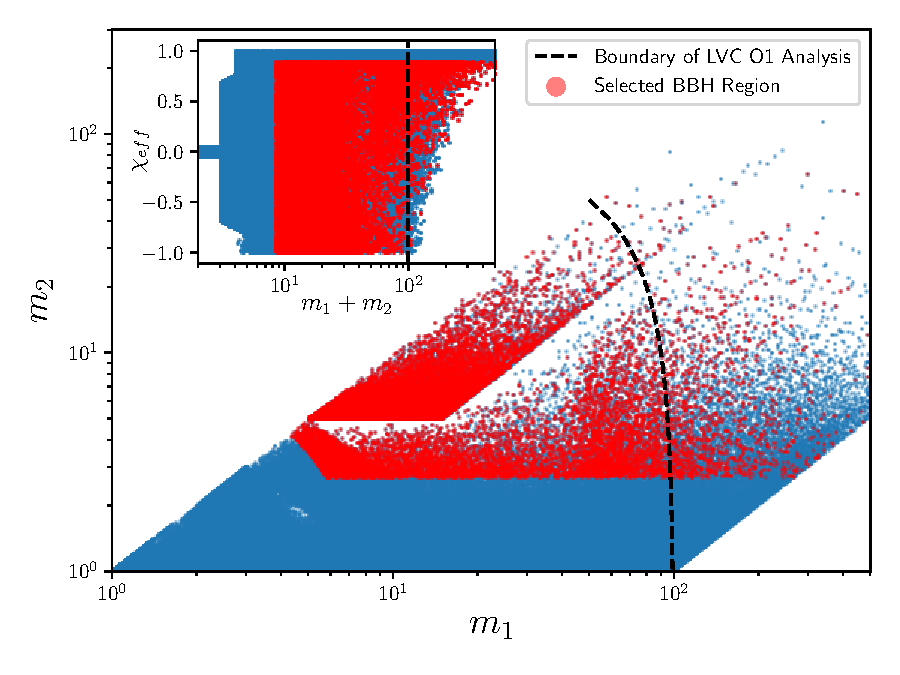
\includegraphics[width=\columnwidth]{figs/chapter5/bank.pdf}
\caption{The component masses and spins of the templates used to search for compact binary mergers. Due to the exclusion of short duration templates, there is a dependency on the total mass searched and its effective spin. For binary black holes with negligible spin, this implies that this study only probes sources with total mass less than ~$200\,\msun$. Visible artifacts due to the procedure for constructing the template bank do not impact performance. Templates which we conservatively consider to produce binary black hole (BBH) candidates consistent with known observations are shown in red as discussed in Sec.~\ref{sec:tdr}. The upper mass boundary of the analysis performed by the LVC in~\cite{TheLIGOScientific:2016pea} is shown
as a black dotted line.}
\label{fig:bank}
\end{figure}

\subsection{Target Search Space}

A discrete bank of gravitational-wave template waveforms~\citep{Owen:1995tm,Owen:1998dk,Brown:2012qf} is used to target binary neutron star,
neutron star--black hole, and binary black hole mergers with total mass from $2-500 M_{\odot}$~\citep{DalCanton:2017ala}. The templates are
parameterized by their component masses $m_{1,2}$ and their dimensionless spins  $\vec{\chi}_{1,2} = c \vec{S}_{1,2}/G m_{1,2}^2$, where
$\vec{S}_{1,2}$ are the spin vectors of each compact object.  For compact objects with component
masses greater than $2 M_{\odot}$, the template bank covers a wide range of spins, with $\chi_{(1,2)z} \in [\pm 0.998]$, where $\chi_{(1,2)z}$ are the components aligned with the orbital angular momentum. For compact objects
with masses less than  $2 M_{\odot}$, the spin is restricted to $\chi_{(1,2)z} \in [\pm 0.05]$~\citep{Brown:2012qf}. Templates that correspond
to sources with a signal duration less than 0.15 seconds (starting from $20\,$Hz) are excluded due to the difficulty in separating candidates arising from
these templates from populations of instrumental glitches~\citep{DalCanton:2017ala}. Consequently, the total mass boundary of the search
depends strongly on the ``effective spin" \citep{Racine:2008qv, Ajith:2009bn},
%
\begin{equation}
\chieff = \frac{\chi_{1z} m_1 + \chi_{2z} m_2}{m_1+m_2}.
\end{equation}
%
This dependence is visible in the distribution of the approximately $400,000$ templates required to cover the space shown in Fig.~\ref{fig:bank}. A dotted line in Fig.~\ref{fig:bank} denotes the upper boundary of the O1 analysis performed in~\cite{TheLIGOScientific:2016pea}. For binaries with total mass greater than $4\,M_\odot$, we use the spinning effective-one-body model (SEOBNRv4)~\citep{Taracchini:2013,Bohe:2016gbl} as template gravitational waveforms. For sources with total masses less than $4M_{\odot}$ we use TaylorF2 post-Newtonian waveforms with phasing accurate to 3.5 post-Newtonian order and the dominant amplitude evolution~\citep{Sathyaprakash:1991mt,Droz:1999qx,Blanchet:2002av,Faye:2012we}. Our choice of template bank discretization causes less than a $10\%$ loss in detection rate for any source within the boundaries of the template bank. Our search assumes that the source can be adequately described by only the dominant gravitational-wave mode, two component masses, non-precessing spins, and negligible eccentricity.

\subsection{Creation and Ranking of Candidate Events}

For each template and each detector, we calculate the matched filter signal-to-noise ratio (SNR) as a function of time $\rho(t)$~\citep{Allen:2005fk}. The template bank is divided into 15 equal sized sub-banks based on the chirp mass $\mathcal{M} = (m_1m_2)^{3/5} / (m_1+m_2)^{1/5}$ of each template. A single-detector ``trigger" is a peak in the SNR time series that is greater than 4 and larger than any other peaks within 1s. For each sub-bank, the loudest 100 triggers (by $\rho$) are recorded in $\sim1$s fixed time windows. This method has been shown to improve search sensitivity, while making the rate of single-detector triggers manageable~\citep{Nitz:2018rgo}. We have found this choice of sub-banks to be an effective method to ensure the analysis can concurrently record triggers from separate regions of parameter space that respond differently to instrumental noise. Other choices are possible.

 We use the data-quality segments provided by the Gravitational-Wave Open Science Center to exclude triggers that occur in times when there are problems with the detectors' data quality~\citep{TheLIGOScientific:2016zmo,TheLIGOScientific:2017lwt}.
 In addition, very loud transient glitches, corresponding to $>100\sigma$ deviations from Gaussian noise, are excised from the strain data according to the procedure of~\cite{Usman:2015kfa} before calculation of the SNR time series. However, there remain many types of transient non-Gaussian noise in the LIGO data which produce triggers with large values of SNR~\citep{Nuttall:2015dqa,TheLIGOScientific:2016zmo,TheLIGOScientific:2017lwt}. 

 For every trigger with $\rho > 5.5$ we calculate the signal consistency test, $\chi^2_r$, introduced in~\cite{Allen:2004gu}. The statistic $\chi^2_r$ divides the matched filter into frequency bands and checks that the contribution from each band is consistent with the expected signal. The statistic takes values close to unity when the data contains either Gaussian noise or the expected signal and larger values for many types of transient glitches. We impose the SNR limit as the $\chi^2_r$ test is generally non-informative when $\rho < 5.5$. The $\chi^2_r$ value is used to re-weight the SNR $\rho$ as~\citep{Babak:2012zx}
%
\begin{equation}
 \tilde{\rho} = \begin{cases} 
        \rho & \mathrm{for}\ \chi^2_r \leq 1 \\
        \rho\left[ \frac{1}{2} \left(1 + \left(\chi^2_r\right)^3\right)\right]^{-1/6}, & 
        \mathrm{for}\ \chi^2_r > 1.
    \end{cases}
\end{equation}
%

For single-detector triggers from templates with total mass greater than 40$M_{\odot}$ we apply an additional test, $\chi^2_{r,sg}$, that determines if the detector output contains power at higher frequencies than the maximum expected frequency content of the gravitational-wave signal~\citep{Nitz:2017lco}. This test is only applied for higher mass systems, since these templates are shorter in duration and more difficult to separate from instrumental noise. For other systems, we set $\chi^2_{r,sg} = 1$. Using this statistic, we apply a further re-weighting as
%
\begin{equation}
\label{eq:sg}
 \hat{\rho} = \begin{cases} 
        \tilde{\rho} & \mathrm{for}\ \chi^2_{r,sg} \leq 4 \\
        \tilde{\rho} (\chi^2_{r,sg} / 4)^{-1/2}, & 
        \mathrm{for}\ \chi^2_{r,sg} > 4.
    \end{cases}
\end{equation}

Candidate events are generated when single-detector triggers occur in both the LIGO Hanford and Livingston data within $12$~ms (the light-travel time between the observatories extended by $2$~ms for signal time-measurement error) and if the triggers are recorded in the same template in each detector~\citep{Usman:2015kfa}.  Following the procedure of~\cite{Nitz:2017svb}, we model the distribution of single detector triggers from each template as an exponentially decaying function, $\lambda(\hat{\rho}, \vec{\theta}^N)$, where $\vec{\theta}^N$ allows the parameters of the exponential to vary as a function of total mass, symmetric mass ratio $\eta=m_1m_2/M^2$, and $\chieff$. This fitted model allows us to rescale $\hat{\rho}$ to better equalize the rate of triggers from each template.

We improve upon the ranking of candidates in~\cite{Abbott:2016ymx,TheLIGOScientific:2016pea} by also taking into account $p^S(\vec{\theta}^S)$, which is the expected distribution of SNR $\rho_H$ and $\rho_L$, phase difference $\phi_{c, H} - \phi_{c, L}$, and arrival time delay $t_{c,H} - t_{c,L}$ between the two LIGO instruments for an astrophysical population~\citep{Nitz:2017svb}. No assumption is made about the distribution of intrinsic source parameters in this term. The primary benefit arises from assuming the population of sources is isotropically distributed in orientation and sky location. The final ranking statistic \rankingstat{} is then calculated as
\begin{equation}\label{eq:genstat}
  \rankingstat \propto \left[ \log p^S(\vec{\theta}^S) - \log \left(\lambda_H(\hat{\rho}_{H},\vec{\theta}^N) \lambda_L(\hat{\rho}_{L}, \vec{\theta}^N)\right) 
  \right] + \mathrm{const.}
\end{equation}
This expression is normalized so that \rankingstat{} approximates the standard network SNR $\rho_c = (\rho_L^2 + \rho_H^2)^{1/2}$ for candidates from regions of parameter space that are not affected by elevated rates of instrumental noise. Candidates from regions affected by elevated rates of noise triggers are down-weighted and assigned a smaller statistic value by this method. As multiple candidates, which arise from different template waveforms, may occur in response to the same signal, we select only the highest ranked candidate within ten seconds. A simpler version of this statistic where the single-detector exponential noise model is only a function of the template duration has also been employed in the analysis of data from LIGO's second observing run~\citep{GW170104, GW170814, Abbott:2017gyy}.

\subsection{Statistical Significance}

The statistical significance of candidate events is estimated by measuring empirically the rate of false alarms (FAR). To measure the noise background rate, we generate additional analyses by time shifting the data from one instrument with respect to the other by multiples of 100 ms. Since this time shift is greater than the maximum astrophysical time of flight between observatories, any candidates produced in these analyses are false alarms. This time shift is much greater than the auto-correlation length of our template waveforms of $\mathcal{O}$(1ms). The time-slid analyses are produced following the same procedure as the search; This is a key requirement for our analysis to produce valid statistical results~\citep{TheLIGOScientific:2016qqj}. The equivalent of more than 50,000 years of observing time can be generated from 5 days of data.

To provide an unbiased measure of the rate of false alarms at least as significant as a potential candidate, the single-detector triggers that compose the candidate event should be included in the background estimation~\citep{2017PhRvD..96h2002C}. However, when a real signal with a large \rankingstat{} is present in the data, the rate of false alarms for candidate events with smaller \rankingstat{} tends to be overestimated. This is due to the fact that the loud single-detector triggers from the real event in one detector form coincidences with noise fluctuations in the other detector, producing loud coincident background events. As in \cite{TheLIGOScientific:2016pea}, an unbiased rate of false alarms can be achieved by a hierarchical procedure whereby a candidate with large \rankingstat{} is removed from the estimation of background for candidates with smaller \rankingstat{}; we use this procedure here.

NEED TO EXPAND THIS PART

\section{Evaluating Candidates based on the Astrophysical Population}
\label{sec:tdr} 

We find two candidate events with
FAR $< 1$ per $50\,000$ years, corresponding to GW150914 and GW151226.
Although FAR does not give the probability that an event is an astrophysical signal,
we can be confident that these events were not caused by chance
coincidence between the detectors. It is possible that these
events were caused by a correlated source between the detectors. However, detailed followup
studies of GW150914 and GW151226 found no correlated noise sources between the detectors
that could be mistaken for a gravitational wave \citep{TheLIGOScientific:2016zmo, Abbott:2016nmj}.

We conclude that GW150914 and GW151226 are astrophysical in origin and use them to constrain the rate of real signals. A ``true discovery rate"
(\tdr{}) can be constructed for less significant events. The \tdr{} is defined as:
%
\begin{equation}
\tdr(\rankingstat) = \frac{\tar(\rankingstat)}{\tar(\rankingstat) + \far(\rankingstat)},
\end{equation}
%
where $\tar(\rankingstat)$ is the rate that signals of astrophysical origin are observed with
a ranking statistic $\geq \rankingstat$ (the ``true alarm rate") and
$\far(\rankingstat)$ is the false alarm rate.

The true discovery rate is the complement of the false discovery rate~\citep{Benjamini:1995ram},
and can be used to estimate the fraction of real signals in a population.
For example, if $\tdr(\rankingstat) = 0.9$, it means that
$90\%$ of events with a ranking statistic $\geq \rankingstat$ are expected to be real signals.  The
\tdr{} is also independent of the observation time.

Note that \tdr{} is not the probability that a particular event is a signal of astrophysical origin \pastro{}. For that, one needs to model the distribution of signals and noise at a given \rankingstat{}. In this work, we use a simple model of these distributions as functions of the ranking statistic \rankingstat{}. Models incorporating additional parameters are also possible, but we do not consider them here. As a function of \rankingstat, \pastro{} can be computed as
%
\begin{equation}
\pastro(\rankingstat) = \frac{\Lambda_S P_S(\rankingstat)}{\Lambda_S P_S(\rankingstat) + \Lambda_N P_N(\rankingstat)},
\end{equation} 
%
where $P_S(\rankingstat)$ and $P_N(\rankingstat)$ are the probabilities of an event having ranking statistic \rankingstat{} 
given the signal and noise hypotheses respectively~\citep{2009MNRAS.396..165G,Farr:2015,Abbott:2016nhf}. $\Lambda_S$ and $\Lambda_N$ are the rates of signal and noise events.

Since no binary neutron star or neutron star--black hole candidates are obtained from a search of the O1 data, here we restrict the calculation of both the \tdr{} and \pastro{} to binary black hole (BBH) observations.
We include signals with total mass $M \geq 10\,\msun$, mass ratio $m_1/m_2 < 5$ (where $m_1 \geq m_2$),
and dimensionless spins $|\chi_{(1,2)z}| <
0.5$. These choices are based on a combination of what has been observed~\citep{TheLIGOScientific:2016pea,GW170104,GW170814,Abbott:2017gyy} and
what is expected from models of isolated binary-star evolution (``field"
binaries). The mass distribution of field binaries is dependent on a number of
unknown parameters, such as the metallicity of the environment~\citep{Belczynski:2014iua}. Generally, it is expected that most binaries are close to equal mass, as typically less than 1
in $\mathcal{O}(10^{3})$ simulated binaries have mass ratio $> 5$ in models of
field-binary evolution \citep{Dominik:2014yma}.  The majority of observations of
nearby X-ray binaries have yielded black holes with masses greater than
$5\,\msun$, which has led to speculation of a ``mass gap" between
3--5$\,\msun$ \citep{Ozel:2010su, Farr:2010tu, Kreidberg:2012ud}. The signals
detected so far by LIGO and Virgo are consistent with this: the smaller component mass
in the lowest-mass system known to date, GW170608, has an estimated mass of
$7^{+2}_{-2}\,\msun$ \citep{Abbott:2017gyy}.

The spin distribution of black holes is not well constrained~\citep{Reynolds:2013qqa}. The component spins
of the most significant binary black holes detected by LIGO and Virgo are
only weakly constrained \citep{TheLIGOScientific:2016pea}. The best measured
quantity related to spin is \chieff{}. All of the BBH gravitational-wave signals
detected so far have $|\chieff| \lesssim 0.2$. A binary with
low \chieff{} may still have component masses with large spin magnitudes,
if the spins are anti-parallel or are purely in the plane of the binary.
However, it seems unlikely that this would be the case for all of the
detections made so far. Hence we include signals that have
component spins with $|\chi_{(1,2)z}| < 0.5$. This is consistent with
recent population synthesis models, which indicate that black holes
must have low natal spin in order to obtain a distribution of \chieff{}
that satisfies gravitational-wave observations \citep{Belczynski:2017gds,Wysocki:2017isg}.

To estimate the rate and distribution of false alarms that arise only
from the region consistent with this selected population of
binary black hole mergers, we must determine which templates are sensitive to these sources.
It is necessary to analyze a simulated set of signals since
the template associated with a particular event is not guaranteed to share the 
true source parameters. We find that the region of the template bank defined by
$M > 8.5\,\msun$, $m_{1,2} > 2.7\,\msun$, and $\chieff < 0.9$ is effective at recovering
this population of sources. This region is shown in Fig.~\ref{fig:bank} in red. 

To estimate the true rate \tar{}, we use the two significant events observed
during O1, GW150914 and GW151226. We do not use any of the O2 events because the full data is
not yet available for analysis, making it difficult to obtain a consistent rate estimate. The total analysis time in O1 was $\sim48$ days, giving $\tar \approx 15 \mathrm{yr}^{-1}$. Given the uncertainty in
this estimate based on only two events, we take the rate of observations as a Poisson process, and choose the lower
95\% bound on \tar{}. This yields a $\tar \approx 2.7 \mathrm{yr}^{-1}$. For the calculation
of the \tdr{} we use this value for all events, independent of their ranking statistic. This means we likely underestimate the \tdr{} for events quieter than GW151226 and GW150914, but this is a conservative bias.

To estimate the probability that a given event is astrophysical in origin \pastro{}, we model
the distribution of signals and noise as a function of \rankingstat. It is reasonable to approximate the signal
probability distribution $P_S(\rankingstat)$ as $\propto \rankingstat^{-4}$~\citep{Schutz:2011tw,Chen:2014yla}.
We normalize the signal number density $\Lambda_S P_S(\rankingstat)$ so that the number of signals
with $\rankingstat$ greater than or equal to some threshold
$\rankingstat^{\dagger}$ is $\approx 2.7 \mathrm{yr}^{-1}$. We make the conservative choice to place
$\rankingstat^{\dagger}$ at the value of the next largest \rankingstat{} value after GW150914 and GW151226. 

To approximate the noise number density $\Lambda_N P_N(\rankingstat)$, we make a histogram of the \rankingstat{}
values of false alarms arising from our selected BBH region. We use only the false alarms which are uncorrelated
with possible candidate events to ensure an unbiased estimate of the mean false alarm rate~\citep{2017PhRvD..96h2002C}.
We fit an exponential decay to this histogram from $8<\rankingstat<9.2$. For \rankingstat{} much less than $8$,
$\Lambda_N P_N$ is not well modeled by an exponential due to the effects of applying a threshold to single-detector
triggers. We note, however, there is only a $ 50 \%$ chance that an event is astrophysical at
\rankingstat{} $\sim 8.6$, and this chance quickly becomes negligible with decreasing \rankingstat. The result of this
procedure is shown in Fig.~\ref{fig:pastro}. We caution that \pastro{} for candidates with
\rankingstat{} $>9.2$ will be sensitive to the form of the model chosen since it is not constrained by
empirically measured false alarms.

While we do not assess the astrophysical probabilities of sources outside our selected BBH region, we are not precluding that such sources exist.
Our \pastro{} is compatible with any model of the true BBH
source distribution that allows for a signal rate to be at least as high as our estimate within the chosen region. This holds irrespective of whatever other kinds of sources may also be permitted.

\begin{figure}[h]
  \centering
    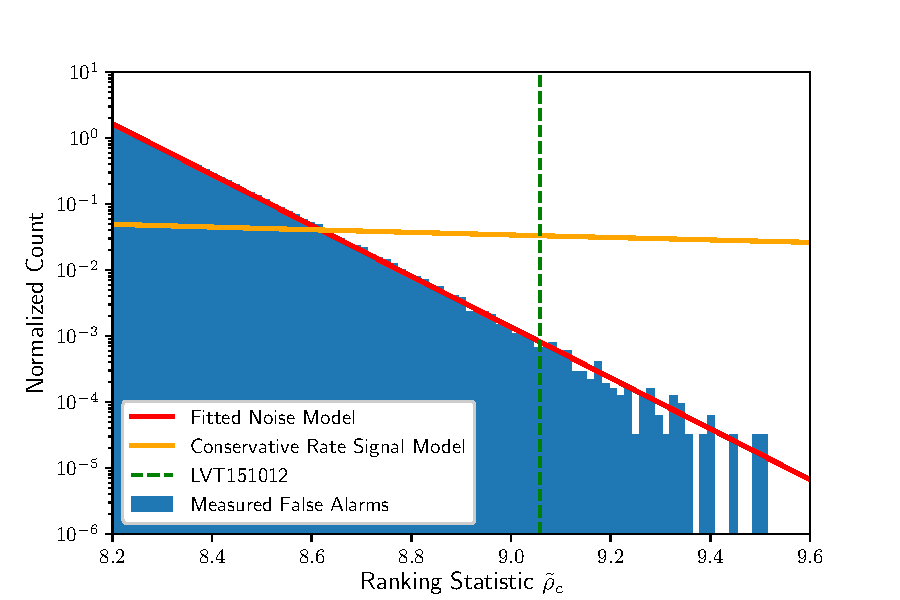
\includegraphics[width=\columnwidth]{figs/chapter5/pastro.pdf}
\caption{The scaled probability distributions of assumed signals and noise as a function of the ranking statistic \rankingstat{} for the analysis containing LVT151012. Blue shows the normalized histogram of empirically measured false alarms that are within our selected BBH region of the template bank, $P_N$. Red is the exponential decay model that has been fitted to this set of false alarms, $P_S \Lambda_S / \Lambda_N$, normalized so that the counts can be directly compared to the noise distribution}. Orange shows the signal model based on our conservative rate of detections. The value of \rankingstat{} for LVT151012 is shown as a dotted green vertical line. The ratio of signal to noise at this value of \rankingstat{} strongly favors the signal model.
\label{fig:pastro}
\end{figure}


\begin{figure}[]
  \centering
    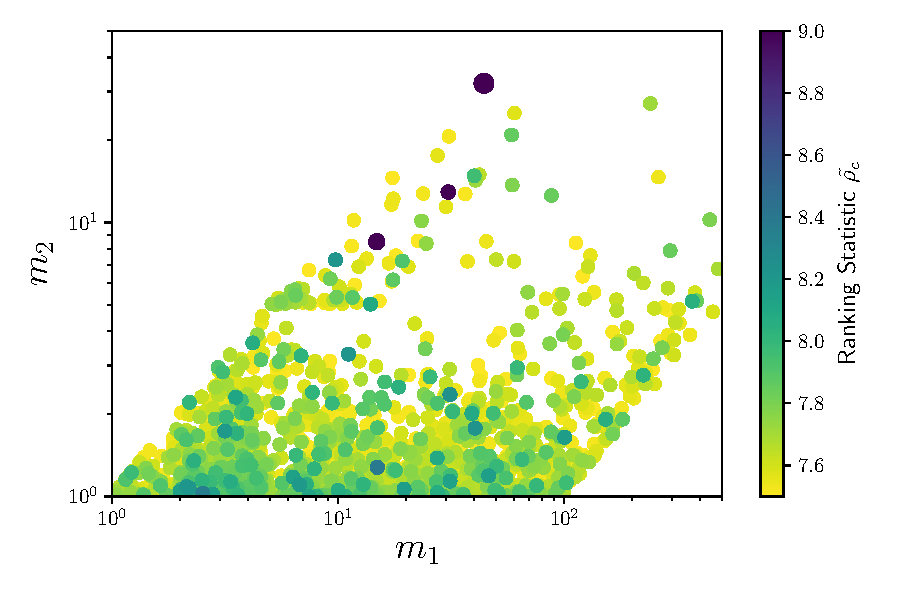
\includegraphics[width=\columnwidth]{figs/chapter5/candidates.pdf}
\caption{Candidate events with a ranking statistic $\rankingstat>7.5$ from the full search for compact binary mergers in O1 data. The colorbar is capped at 9. The three BBH mergers are clearly visible in the plots, while the remaining events are largely distributed according to the density 
of the template bank.}
\label{fig:bankcandidates}
\end{figure}


\begin{table*}[width=\columnwidth]
  \begin{center}
    \caption{Candidate events from the full search for compact binary mergers in O1 data. Candidates are sorted by FAR evaluated for the entire bank of templates. The FAR of the top two candidates is limited only by the amount of background time estimated, and only differ due to the variation in time available in their respective analyses to create background. The parameters of the template associated with each candidate are listed. Note that these are not intended as a rigorous estimation of the source parameters. Masses are given in the detector frame.}
    \label{table:complete}
\begin{tabular}{lllllllll}[width=\columnwidth]
Designation & Julian Date & $FAR^{-1} (yr)$ & \rankingstat{} & $\rho_H$ & $\rho_L$ & $m_1$ & $m_2$ & $\chieff{}$ \\ \hline
150914+09:50:45UTC & 2457279.910665 &  $>$66000 & 18.45 & 19.67 & 13.38 & 44.21 & 32.16 & 0.09 \\
151226+03:38:53UTC & 2457382.652426 &  $>$59000 & 11.62 & 10.73 & 7.43 & 14.83 & 8.50 & 0.24 \\
151012+09:54:43UTC & 2457307.913420 &     24 & 9.06 & 6.96 & 6.71 & 30.75 & 12.89 & -0.05 \\
151019+00:23:16UTC & 2457314.516585 &      0.060 & 8.39 & 6.81 & 5.47 & 14.93 & 1.27 & 0.11 \\
150928+10:49:00UTC & 2457293.951122 &      0.042 & 8.37 & 6.05 & 6.34 & 2.53 & 1.02 & -0.70 \\
151218+18:30:58UTC & 2457375.271929 &      0.029 & 8.24 & 7.11 & 5.38 & 31.29 & 2.35 & -0.00 \\
160103+05:48:36UTC & 2457390.742504 &      0.026 & 8.22 & 6.01 & 6.60 & 9.75 & 7.29 & 0.49 \\
151202+01:18:13UTC & 2457358.554740 &      0.025 & 8.23 & 6.54 & 5.73 & 40.42 & 1.77 & -0.26 \\
160104+03:51:51UTC & 2457391.661424 &      0.021 & 8.19 & 5.80 & 6.39 & 6.76 & 1.10 & -0.51 \\
151213+00:12:20UTC & 2457369.508985 &      0.019 & 8.22 & 5.70 & 7.24 & 11.12 & 3.30 & -0.79 \\
150923+07:10:59UTC & 2457288.799711 &      0.014 & 8.20 & 6.78 & 5.84 & 2.14 & 1.08 & 0.65 \\
151029+13:34:39UTC & 2457325.066149 &      0.014 & 8.21 & 6.83 & 5.23 & 2.19 & 1.07 & -0.27 \\
151206+14:19:29UTC & 2457363.097291 &      0.013 & 8.17 & 5.80 & 6.37 & 100.60 & 1.64 & 0.98 \\
151202+15:32:09UTC & 2457359.147751 &      0.012 & 8.14 & 5.93 & 6.41 & 6.33 & 1.18 & -0.59 \\
151012+06:30:45UTC & 2457307.771774 &      0.011 & 8.19 & 6.74 & 5.70 & 3.16 & 1.73 & -0.15 \\
151116+22:41:48UTC & 2457343.446120 &      0.010 & 8.14 & 5.79 & 6.64 & 2.00 & 1.04 & -0.45 \\
151121+03:34:09UTC & 2457347.649138 &      0.010 & 8.12 & 6.48 & 5.78 & 7.43 & 1.00 & -0.86 \\
150922+05:41:08UTC & 2457287.737317 &      0.010 & 8.16 & 6.05 & 6.34 & 2.78 & 1.02 & 0.17 \\
151008+14:09:17UTC & 2457304.090202 &      0.008 & 8.16 & 5.84 & 6.10 & 46.38 & 1.19 & 0.38 \\
151127+02:00:30UTC & 2457353.584101 &      0.008 & 8.10 & 6.28 & 5.44 & 39.12 & 2.01 & 0.99 \\


\end{tabular}
  \end{center}
\end{table*}


\section{Results}
\label{sec:results}


The results presented here are generated using the data from the first observing run of Advanced LIGO which ran from September 12, 2015 to January 19, 2016. We divide the 16~kHz LIGO open data into 9 consecutive periods of time and search each time period independently so that each analysis contains roughly five days of observing time. This time interval is set by the disk and memory requirements of the search pipeline, but it is sufficient to estimate the FAR of candidate events to better than 1 in 50,000 years. It is possible to combine these time intervals during the analysis to improve this limit, but we have not done so here. Our analysis is restricted to times marked as observable by the metadata provided by the Gravitational-Wave Open Science Center. After accounting for times which are marked as not analyzable, there remain $\sim48.1$ days of data when both the Hanford and Livingston LIGO instruments were operating.

The top candidate events by FAR from the full search are given in Table~\ref{table:complete}. There are three candidates which are statistically significant. These are the binary black hole mergers GW150914, LVT151012, and GW151226, which were previously reported in~\cite{TheLIGOScientific:2016pea,Abbott:2016blz,Abbott:2016nmj}. The false alarm rates for GW150914 and GW151226 of 1 per 66,000 and 1 per 59,000 years, respectively, are limits based on the amount of background time available in their respective analysis. These limits are less stringent than those reported in~\cite{TheLIGOScientific:2016pea} as we have created less background time. There are no other individually convincing candidates. Fig.~\ref{fig:bankcandidates} shows candidate events with $\rankingstat > 7.5$. The three binary black hole mergers stand out from the other candidate events and are clustered in a portion of the parameter space that is analyzed with relatively few template waveforms.



\begin{table*}[]
  \begin{center}
    \caption{Candidate events consistent with the selected population of binary black holes. There are three binary black hole mergers above a threshold corresponding to a true discovery rate of $99.92\%$. The third most significant event, LVT151012, has a 97.6\% probability of
    being astrophysical in origin. Note that the FARs indicated do not reflect the false alarm rate for the full search, but instead for the limited region of the template bank indicated in red in Fig.~\ref{fig:bank}. The FARs listed for the top two events are limited
    by the background time generated and so are identical to those in Table~\ref{table:complete}.}
    \label{table:bbh}
\begin{tabular}{lllllllllll}[width=\columnwidth]
Designation & Julian Date & $\pastro{}$ & TDR & $FAR^{-1} (yr)$ & \rankingstat{} & $\rho_H$ & $\rho_L$ & $m_1$ & $m_2$ & $\chieff{}$ \\ \hline
150914+09:50:45UTC & 2457279.910665 & - & - &  $>$66000 & 18.45 & 19.67 & 13.38 & 44.21 & 32.16 & 0.09\\
151226+03:38:53UTC & 2457382.652426 & - & - &  $>$59000 & 11.62 & 10.73 & 7.43 & 14.83 & 8.50 & 0.24\\
151012+09:54:43UTC & 2457307.913420 & 0.976 & 0.999 &    446 & 9.06 & 6.96 & 6.71 & 30.75 & 12.89 & -0.05\\
160103+05:48:36UTC & 2457390.742504 & 0.061 & 0.517 &      0.396 & 8.22 & 6.01 & 6.60 & 9.75 & 7.29 & 0.49\\
151213+00:12:20UTC & 2457369.508985 & 0.047 & 0.455 &      0.309 & 8.22 & 5.70 & 7.24 & 11.12 & 3.30 & -0.79\\
151216+18:49:30UTC & 2457373.284799 & 0.017 & 0.223 &      0.106 & 8.09 & 6.10 & 6.01 & 13.92 & 5.03 & -0.41\\
151222+05:28:26UTC & 2457378.728506 & 0.012 & 0.169 &      0.075 & 8.03 & 5.67 & 6.46 & 6.86 & 3.26 & -0.74\\
151217+03:47:49UTC & 2457373.658627 & 0.006 & 0.088 &      0.036 & 7.96 & 6.69 & 5.57 & 40.02 & 14.77 & 0.84\\
151009+05:06:12UTC & 2457304.713060 & 0.005 & 0.087 &      0.035 & 7.99 & 5.66 & 5.90 & 25.55 & 2.73 & -0.05\\
151220+07:45:36UTC & 2457376.823761 & 0.003 & 0.053 &      0.021 & 7.87 & 6.55 & 5.39 & 17.50 & 6.17 & 0.82\\
151104+04:12:55UTC & 2457330.676062 & 0.003 & 0.053 &      0.021 & 7.91 & 5.94 & 6.33 & 19.25 & 7.22 & 0.71\\
151120+16:20:06UTC & 2457347.181049 & 0.003 & 0.047 &      0.018 & 7.86 & 6.11 & 5.44 & 5.49 & 3.10 & 0.79\\
151216+09:24:16UTC & 2457372.892271 & 0.003 & 0.045 &      0.017 & 7.86 & 5.76 & 5.66 & 58.56 & 20.84 & 0.66\\
151128+14:37:02UTC & 2457355.109478 & 0.003 & 0.040 &      0.016 & 7.83 & 6.79 & 5.02 & 9.25 & 6.22 & -0.87\\
160109+08:08:42UTC & 2457396.839798 & 0.003 & 0.035 &      0.014 & 7.82 & 5.24 & 6.23 & 24.29 & 3.45 & -0.98\\
160111+22:49:34UTC & 2457399.451507 & 0.003 & 0.035 &      0.013 & 7.82 & 5.10 & 6.55 & 5.75 & 3.43 & 0.23\\
151124+11:25:19UTC & 2457350.976339 & 0.002 & 0.033 &      0.013 & 7.81 & 5.65 & 6.27 & 98.89 & 3.89 & 0.45\\
150912+15:39:02UTC & 2457278.152523 & 0.002 & 0.032 &      0.012 & 7.84 & 6.23 & 5.23 & 9.86 & 5.33 & -0.01\\
151006+06:06:50UTC & 2457301.755168 & 0.002 & 0.031 &      0.012 & 7.89 & 6.77 & 5.47 & 11.59 & 5.31 & -0.05\\
151015+01:40:52UTC & 2457310.570466 & 0.002 & 0.029 &      0.011 & 7.85 & 5.37 & 5.92 & 87.87 & 12.52 & 0.75\\

\end{tabular}
  \end{center}
\end{table*}

\subsection{Binary Black Hole Candidates}

Given that there are two binary black hole mergers (GW150914 and GW151226 ) that are well established from their
statistical significance, we can estimate the rate of detecting binary black hole mergers by this analysis. Candidate
events that are consistent with our selected binary black hole population are listed in
Table~\ref{table:bbh}. We estimate the false alarm rate of events for just this region of the analysis, and using our
estimate of the true rate of detections, calculate the true discovery rate as a function of ranking statistic. The
\tdr{} at the ranking statistic of the fourth most significant candidate is 0.52. This means that only 52\% of
candidates with \rankingstat{} at least as large are expected to be of astrophysical origin. For each candidate we estimate its
individual probability of being astrophysical in origin, \pastro{}. The fourth event has only a 6$\%$ chance of being
astrophysical. We do not report \pastro{} and \tdr{} values for the top two events since these events
are assumed to be signals in the construction of these statistics.


\subsection{Revisiting LVT151012}

LVT151012 was first announced in~\cite{TheLIGOScientific:2016qqj}, with a FAR
of 1 per 2.3 years. Our improved methods yield a false alarm rate for LVT151012
of 1 per 24 years. Restricting attention to our selected BBH region, which is
consistent with the other observed binary black hole mergers, gives a FAR for
LVT151012 in this region alone of 1 per 446 years. We combine this FAR  with
our conservative estimate of the rate of detections to estimate that 99.92\% of
binary black hole merger candidates at least as significant as LVT151012 are
astrophysical in origin. We also estimate the probability that specifically
LVT151012 is astrophysical in origin to be 97.59$\%$.

These measures both depend on our selected region of binary black hole sources
and our estimate of the rate of true detections, but we believe our choices for
both of these to be conservative. The FAR of 1 per 446 years is not a
statistical statement about the search as a whole and is used only in
comparison against the rate of real signals within this same region. Selecting
different boundaries for this region would yield a different FAR. However,
assuming that the false alarm rate and true alarm rate are both approximately
uniform in this region, then \pastro{} and \tdr{} will not change.


As data from future observing runs becomes available, it will be possible to more precisely estimate this rate in a consistent way, and improve our estimate of this event's significance.  We have modeled our signal distribution and population of false alarms as being characterized by the ranking statistic \rankingstat{} alone. An improved model could take into account the variation over the parameter space and in time. Fig.~\ref{fig:pastro} shows the probability distribution of our noise and signal models for the analysis which contains LVT151012. Compared to the \pastro{} reported in~\cite{TheLIGOScientific:2016pea} of 87\%, our analysis has improved the ranking of candidate events, the boundaries of our selected BBH distribution differ from what was used there, and we use a more conservative estimate of the signal rate. Given a \pastro{} value of 97.6$\%$ we conclude that LVT151012 is astrophysical in origin. For comparison, if we had chosen the rate of observed mergers to be $\approx 15 \mathrm{yr}^{-1}$, which is the linear extrapolation of two detections in 48 days, we would find that LVT151012 had a $99.6\%$ probability of astrophysical origin.

\section{Data Release}
\label{sec:datarelease}

The 1-OGC catalog contains $\sim 150,000$ candidate events. Our supplemental materials online provide the complete combined set of binary neutron star, neutron star--black hole, and binary black hole candidates~\citep{1-OGC}. A separate listing of the candidates from our selected BBH region is also made available. Each candidate is assigned an identifying name constructed from the date and UTC time. The vast majority of these candidates are not astrophysical in origin. To help distinguish between possible sources we provide our ranking statistic $\rankingstat$ along with our estimate of the false alarm rate for each candidate. We also provide information such as the SNR observed by each instrument, the time of arrival, measured phases, and the results of our set of signal consistency tests. The periods of time that were analyzed are also provided. We also provide the PyCBC pipeline configuration files that allow our analysis to be reproduced.


\section{Discussion}

We present a full catalog of gravitational-wave events and candidates from a PyCBC-based, templated, matched-filter search of the LIGO O1 open data.  Our analysis represents an improvement over that of \cite{TheLIGOScientific:2016pea,Abbott:2016ymx} by using improved ranking of candidates by considering phase, amplitude and time delay consistency, an improved background model and a template bank targeting a wider range of sources \citep{Nitz:2017svb, Nitz:2017lco,DalCanton:2017ala}. We independently verify the discovery of GW150914 and GW151226 and report an improved significance of the candidate event LVT151012, which we claim should be viewed as a confident detection.  Apart from these three signals, none of the other candidate events are individually significant in our analysis.  All of these candidates are listed in our catalog available at \release{}, along with tools for exploring and using it. Complete gravitational-wave event catalogs of this nature will become important tools in multi-messenger astronomy.

A  larger data set from the second observing run of LIGO and Virgo already exists. Individual detections have been published, and short periods of data around the detections are available publicly.  However, the bulk of this data has not yet been released publicly. It will be possible to create a similar open catalog with the most up-to-date analysis tools when these data are released.


We thank Thomas Dent and Sumit Kumar for useful discussions and comments. We thank Stuart Anderson, Jonah Kannah, and Alan Weinstein for help accessing data from the Gravitational-Wave Open Science Center.  We acknowledge the Max Planck Gesellschaft for support and the Atlas cluster computing team at AEI Hannover. Computations were also supported by Syracuse University and NSF award OAC-1541396. DAB acknowledges NSF awards PHY-1707954, OAC-1443047, and OAC-1738962 for support. SR acknowledges NSF award PHY-1707954 and OAC-1443047 for support. RW acknowledges NSF award OAC-1823378 for support. 
This research has made use of data, software and/or web tools obtained from the Gravitational Wave Open Science Center (https://www.gw-openscience.org), a service of LIGO Laboratory, the LIGO Scientific Collaboration and the Virgo Collaboration. LIGO is funded by the U.S. National Science Foundation. Virgo is funded by the French Centre National de Recherche Scientifique (CNRS), the Italian Istituto Nazionale della Fisica Nucleare (INFN) and the Dutch Nikhef, with contributions by Polish and Hungarian institutes.


\Chapter{Pressure-Gravity Mode Instability in GW170817}
\label{ch:pg_modes}
\section{Introduction} \label{sec:intro}
The discovery of the binary neutron star merger GW170817 \citep{TheLIGOScientific:2017qsa} has given us a new way to explore the physics of neutron stars. Recent studies have measured the star's tidal deformability and placed constraints on the equation of state of the neutron stars~\citep{TheLIGOScientific:2017qsa,Tews:2018iwm,Most:2018eaw,Raithel:2018ncd,de2018tidal,Abbott:2018exr,Abbott:2018wiz,Radice:2018ozg,LIGOScientific:2019eut,Capano:2019eae}.
\cite{Weinberg:2013pbi} have suggested that the star's tidal deformation can induce nonresonant and nonlinear daughter wave excitations in $p$- and $g$-modes of the neutron stars via a quasi-static instability. This instability would remove energy from a binary system and possibly affect the phase evolution of the gravitational waves radiated during the inspiral. Although \cite{Venumadhav:2013nla} concluded that there is no quasi-static instability and hence no effect on the inspiral, \cite{Weinberg:2015pxa} claims that the instability can rapidly drive modes to significant energies well before the binary merges. However, the details of the instability saturation are unknown and so the size of the effect of the $p$-$g$ mode coupling on the gravitational-waveform is not known~\citep{Weinberg:2015pxa}. The discovery of the binary neutron star merger GW170817 by Advanced LIGO and Virgo provides an opportunity to determine if there is evidence for nonlinear tides from $p$-$g$ mode coupling during the binary inspiral.

Since the physics of the $p$-$g$ mode instability is uncertain, \cite{Essick:2016tkn} developed a parameterized model of the energy loss due to nonlinear tides. This model is parameterized by the amplitude and frequency dependence of the energy loss, and the gravitational-wave frequency at which the instability saturates and the energy loss turns on. For plausible assumptions about the saturation, \cite{Essick:2016tkn} concluded that $> 70\%$ of binary merger signals could be missed if only point-particle waveforms are used, and that neglecting nonlinear tidal dynamics may significantly bias the measured parameters of the binary. Bayesian inference can be used to place constraints on nonlinear tides during the inspiral of GW170817. An analysis by \cite{abbott2019constraining} computed Bayes factors that investigate whether the GW170817 signal is more likely to have been generated by a model which includes nonlinear tides or one which does not. \cite{abbott2019constraining} find a Bayes factor of order unity, and conclude that the GW1701817 signal is consistent with both a model that neglects nonlinear tides and with a model that includes energy loss from a broad range of $p$-$g$ mode parameters. However, the prior space used in this analysis includes a large region of  parameter space where the amplitude of the effect produces a gravitational-wave phase shift that is extremely small. In this case, a waveform that includes $p$-$g$ mode parameters will have a likelihood that is identical to the likelihood of the waveform without the $p$-$g$ mode instability. The $p$-$g$ mode model extends the standard waveform model by adding additional parameters that describe the nonlinear tidal effects. However, when including new parameters in a hypothesis if the likelihood does not vary across large portions of the prior volume for these new parameters relative to the likelihood of the original model, then the Bayes factor will not penalize this additional prior volume, nor will it penalize any extraneous parameters in the model (see e.g. \cite{kass1995bayes,hobson2010bayesian}). We examine prior space of $p$-$g$ model used by \cite{abbott2019constraining} and find that although the $p$-$g$ model model contains regions that are not consistent with the standard model, there are large regions of the prior space where the likelihood is high because the $p$-$g$ mode model is degenerate with the standard model. These regions of prior space dominate the evidence and hence the Bayes factor neither favors nor disfavors the inclusion of $p$-$g$ mode parameters.

We investigate a variety of different prior distributions on the $p$-$g$ mode parameters beginning with a prior distribution that is similar to that tested in~\cite{abbott2019constraining} and includes large regions of the parameter space that produce a negligible gravitational-wave phase shift. When comparing the evidence for this model with the standard waveform model used by \cite{de2018tidal} we find a Bayes factor of order unity, as expected. We then investigate a prior distribution in which the $p$-$g$ mode instability parameters are constrained to induce a phase shift to the waveform that is greater than $0.1$ radians. This phase shift is calculated from the time the waveform enters the sensitive band of the detector to the time when the waveform reaches the innermost stable circular orbit. We choose this threshold to exclude trivial regions of the parameter space that produce a non-measurable effect. However, we again find a Bayes factor of order unity when compared to the model hypothesis that does not model the $p$-$g$ mode instability. Investigation of these results showed that this is due to parameter degeneracies between the $p$-$g$ mode model and the intrinsic parameters of the standard waveform model.

Finally, we reduce the prior space to contain only the regions where the $p$-$g$ mode waveform is not degenerate with the standard model by computing the fitting factor~\citep{Apostolatos:1995pj} of $p$-$g$ signals against a set of standard waveforms. We do this to restrict the region of parameter space to that where the $p$-$g$ effect is \emph{measurably} distinct from a model that neglects nonlinear tides. We calculate the Bayes factor as a function of the fitting factor. We find that as the $p$-$g$ mode parameter space is restricted to exclude regions that have a high fitting factor with standard waveforms, the Bayes factor decreases significantly. Regions of the nonlinear tide parameter space that have a fitting factor of less than 99\% (98.5\%) are strongly disfavored by a Bayes factor of 15 (25).  While certain prior distributions of $p$-$g$ mode parameters are consistent with the data, we find that these distributions are ones that contain large regions of non-measurable parameter space either because the effect produced is too small to measure, or the effect is degenerate with other parameters of the standard model. We conclude that the consistency of the GW170817 signal with the model of \cite{Essick:2016tkn} is due to degeneracies and that regions where non-linear tides produce a measurable effect are strongly disfavored.

\section{Waveform model}
\label{sec:waveform}

As two neutron stars orbit each other, they lose orbital energy $E_\mathrm{orbital}$ due to gravitational radiation $\dot{E}_{GW}$. The gravitational waveform during the inspiral is well modeled by post-Newtonian theory~(see e.g. \cite{Blanchet:2013haa}).  The effect of the $p$-$g$ mode instability is to dissipate orbital energy by removing energy from the tidal bulge of the stars~\citep{Weinberg:2013pbi,Weinberg:2015pxa,Essick:2016tkn}. Once unstable, the coupled $p$- and $g$-modes are continuously driven by the tides, giving rise to an extra energy dissipation $\dot{E}_{NL}$ for each star in the standard energy-balance equation~\citep{Peters:1963ux} 
\begin{equation}
\dot{E}_\mathrm{orbital} = -\dot{E}_\mathrm{GW} - \dot{E}^1_\mathrm{NL} - \dot{E}^2_\mathrm{NL}.
\label{eqn:energy_bal}
\end{equation}
Since the details of how the nonlinear tides extract energy from the orbit is not known, \cite{Essick:2016tkn} constructed a simple model of the energy loss and calculated plausible values for the model's parameters. In this model, the rate of orbital energy lost during the inspiral is modified by 
\begin{equation}\label{eqn:energy_nl}
\dot{E}_\mathrm{NL} \propto A f^{n+2} \Theta (f - f_0),
\end{equation}
where $A$ is a dimensionless constant that determines the overall amplitude of the energy loss, $n$ determines the frequency dependence of the energy loss, and $f_0$ is the frequency at which the $p$-$g$ mode instability saturation occurs and the effect turns on. By solving Eq.~(\ref{eqn:energy_bal}), \cite{Essick:2016tkn} computed the leading order effect of the nonlinear tides on the gravitational-wave phase as a function of $A$, $n$, and $f_0$. In this analysis, they allowed each star to have independent values of $A$, $f_0$, and $n$, but found that the energy loss due to nonlinear tides depends relatively weakly on the binary's mass ratio. Hence, they consider a model that performs a Taylor expansion in the binary's component mass~\citep{DelPozzo:2013ala} and include only the leading order terms in the binary's phase evolution. Given this, we parameterize our nonlinear tide waveform with a single set of parameters $A$, $n$, and $f_0$, by setting $\dot{E}^1_\mathrm{NL} = \dot{E}^2_\mathrm{NL}$. We  keep only the leading order nonlinear tide terms when we obtain the quantities $t(f)$ and $\phi(f)$ used to compute the stationary phase approximation~\citep{Sathyaprakash:1991mt,Droz:1999qx,Lindblom:2008cm}. This approach is reasonable for GW170817, since both neutron stars have similar masses and radii~\citep{de2018tidal}.

The dependence of $A$, $n$, and $f_0$ on the star's physical parameters is not known~\citep{Weinberg:2015pxa}. \cite{Essick:2016tkn} estimate that plausible parameter ranges are $A \lesssim 10^{-6}$, $0 \lesssim n \lesssim 2$, and $30 \lesssim f_0 \lesssim 80$ Hz. \cite{Zhou:2018tvc} found that the frequency at which the instability begins to grow is equation-of-state dependent and can occur at gravitational-wave frequencies as high as $700$~Hz. \cite{Andersson:2017iav} suggest that the instability may only act during the late stages of inspiral, (above $300$~Hz), otherwise the large energy dissipation will cause the temperature of the neutron stars to be very large. 

In this paper, we compare two models for the gravitational waves radiated by GW170817. The first is the standard restricted stationary-phase approximation to the Fourier transform of the gravitational waveform $\tilde{h}(f)$, known as the TaylorF2 waveform~\citep{Sathyaprakash:1991mt}. We begin with the same waveform model used by \cite{de2018tidal}, which is accurate to 3.5 PN order in the orbital phase, 2.0 PN order in spin-spin, self-spin and quadrupole-monopole interactions, 3.5 PN order in spin-orbit coupling, and includes the leading and next-to-leading order corrections from the star's tidal deformability~\citep{Kidder:1992fr,Blanchet:1995ez,Blanchet:2004ek,Buonanno:2009zt,Arun:2008kb,Marsat:2013caa,Bohe:2013cla,Bohe:2015ana,Mikoczi:2005dn, Flanagan:2007ix,Vines:2011ud}. We then construct a second model that adds the leading order effect of nonlinear tides computed using the model of \cite{Essick:2016tkn}. Below we detail the construction of this second model, by computing the leading order nonlinear tidal Fourier phase term for the TaylorF2 model as well as the leading order nonlinear tidal energy dissipation.

We begin our derivation with the energy balance equation presented in \cite{Essick:2016tkn},
\begin{equation}\label{eqn_app:energy_bal}
\dot{E}_{orbit} = -\dot{E}_{GW} - 2 \dot{E}_{NL},
\end{equation}
for $\dot{E}_{orbit}$ being the rate of energy loss of a quasi-circular orbit, $\dot{E}_{GW}$ being the energy rate loss due to gravitational waves in the point-particle model, and $\dot{E}_{NL}$ being the rate of energy loss from each star's $p$-$g$ mode instability. We assume that the energy losses from $p$-$g$ mode instability will be comparable in each star. The $\dot{E}$ notation refers to the derivative of the energy with respect to time. We now give explicit values to these energy rates with respect to gravitational wave frequency, $f$.
\begin{equation}\label{eqn:e_orbit_decay}
\dot{E}_{\mathrm{orbit}} = - \frac{G^{2/3} \pi^{2/3} \mathcal{M}^{5/3} \dot{f}}{3 f^{1/3}}
\end{equation}
is the orbital energy decay. The gravitational wave energy rate as a function of frequency is given as:
\begin{equation}\label{eqn:e_gw_decay}
\dot{E}_{\mathrm{GW}} = \frac{32 G^{7/3} \left(\pi \mathcal{M} f\right)^{10/3}}{5 c^5}
\end{equation}
Finally, we take from \cite{Essick:2016tkn} that each star, indexed by i, should have an energy dissipation rate of
\begin{equation}\label{eqn:e_nl_decay}
\dot{E}_{\mathrm{NL}, i} = \frac{(2G m_i)^{2/3}m_1 m_2}{M} (\pi f_{\mathrm{ref}})^{5/3} A \left (\frac{f}{f_{\mathrm{ref}}} \right )^{n+2} \Theta(f - f_0) 
\end{equation}
where $m_i$ is the component mass of the neutron star, $M$ is the total mass ($M$ = $m_1$ + $m_2$). The other parameters are fully described in the Introduction. Assuming that the binaries have equal mass in Eq. \ref{eqn:e_nl_decay} and solving for $\dot{f}$, we arrive at the following expression.
\begin{equation}\label{eqn:f_dot}
\frac{df}{dt} =  \pi \left ( \frac{f}{f_{\mathrm{ref}}} \right )^{7/3} \, f_{\mathrm{ref}}^2 \times \left [ \frac{96}{5} \left ( \frac{G \mathcal{M} \pi f_{\mathrm{ref}}}{c^3}\right )^{5/3} \left (\frac{f}{f_{\mathrm{ref}}} \right )^{4/3} + 6 A \left (\frac{f}{f_{\mathrm{ref}}} \right )^{n} \Theta(f - f_0) \right ]
\end{equation}

Given this expression, we can now consider a time domain signal of the form, $h(t)$ = $A(t)$ $e^{\phi(t)}$, where $h(t)$ is the strain of the gravitational wave at some time t before merger, $A(t)$ is the amplitude of the gravitational wave strain at that same time, and $\phi(t)$ is the orbital phase of the binaries\cite{2008gravitational}. The stationary phase approximation lets us approximate the Fourier transform of this time signal according to the following:
\begin{equation}\label{eqn:SPA}
\tilde{h}(f) = \int_{-\infty}^{\infty} h(t) dt = \int_{-\infty}^{\infty} A(t) e^{-2\pi i ft + \phi(t)} df \approx \tilde{B}(f) e^{-i\Psi(f)}
\end{equation}
where $\tilde{B}(f)$ is the Fourier amplitude of the frequency domain waveform, and $\Psi(f)$ is the Fourier phase of the frequency domain waveform. The full expression for $\Psi(f)$ is
\begin{equation}\label{eqn:SPA_Phase}
\Psi(f) = 2\pi f t(f) - \phi(f).
\end{equation}

One can derive $t(f)$ by solving the differential equation given in Eq. \ref{eqn:f_dot}. For convenience we redefine and reorganize this differential equation as:
\begin{equation}\label{eqn:unitless_f_dot}
\int_{t_c}^t dt = \int_{x_c}^{x}  \frac{f_{\mathrm{ref}}}{\kappa} \frac{x^{-7/3} dx}{\alpha x^{4/3} +  \Theta(x - x_0) \beta x^n}
\end{equation}
where $x$ = $f / f_{\mathrm{ref}}$, $dx$ = $df / f_{\mathrm{ref}}$, $x_0$ = $f_0 / f_{\mathrm{ref}}$, and $\kappa$ = $\pi f_{\mathrm{ref}}^2$. The integration bounds are the time of coalescence ($t_c$ = 0) to some time $t$ prior to merger, and from dimensionless frequency at coalescence ($x_c$ = $f_c / f_{\mathrm{ref}}$ = $\infty$) to some dimensionless frequency $x$ prior to merger. Here $\alpha$ and $\beta$ are given by the following expressions:
\begin{equation}
\alpha = \frac{96}{5} \left ( \frac{G \pi \mathcal{M} f_{\mathrm{ref}}}{c^3} \right )^{5/3}
\end{equation}

\begin{equation}
\beta = 6 A
\end{equation}

We can simplify the differential equation given in Eqn. \ref{eqn:unitless_f_dot} if we assume that the point particle gravitational wave contribution dominates ($\alpha$ $\gg$ $\beta$), we take a power series expansion assuming large $\alpha$ relative to $\beta$. This gives to lowest order in $\beta$:
\begin{equation}\label{eqn:dt_app}
\int_{t_c}^t dt = \int_{x_c}^{x} \frac{f_{\mathrm{ref}}}{\kappa} \left (\frac{1}{\alpha x^{11/3}} +  \frac{\Theta(x - x_0) \beta x^{n-5}}{\alpha^2 (n-5)} \right ) dx
\end{equation}
The first term in Eq. \ref{eqn:dt_app} corresponds to the zeroth order post-Newtonian result from the point-particle model. Integrating the second term and respecting the $\Theta(x-x_0)$ so as to align the waveform at merger ($t=0$), we arrive at the leading order contribution of $p$-$g$ mode instability to $t(f)$:
The first term in Eq. \ref{eqn:dt_app} corresponds to the zeroth order post-Newtonian result from the point-particle model. Integrating the second term and respecting the $\Theta(x-x_0)$ so as to align the waveform at merger ($t=0$), we arrive at the leading order contribution of $p$-$g$ mode instability to $t(f)$:
\begin{equation}\label{eqn:t_of_f_app}
\Delta t(f) = \left \{
              \begin{array}{ll}
              \frac{-25}{1536} \frac{1}{\pi} \frac{A}{n-4} \left ( \frac{G \mathcal{M} \pi f_{\mathrm{ref}}}{c^3} \right )^{-10/3}\left ( \frac{f_0}{f_{\mathrm{ref}}} \right )^{n-4}, &\quad   f < f_0 \\ \\
              \frac{-25}{1536} \frac{1}{\pi} \frac{A}{n-4} \left ( \frac{G \mathcal{M} \pi f_{\mathrm{ref}}}{c^3} \right )^{-10/3}\left ( \frac{f}{f_{\mathrm{ref}}} \right )^{n-4}, &\quad  f \ge f_0
              \end{array}
              \right.
\end{equation}

Following a similar methodology we can calculate $\phi(f)$ via $d\phi$ = $2 \pi f dt$ = $2 \pi (f/\dot{f}) df$. Taking the same power series expansion, integrating so that the waveform coalesces at $t = 0$, and examining the leading order contribution from $p$-$g$ mode instability we arrive at
\begin{equation}\label{eqn:dphi_app}
\int_{\phi_c}^\phi d\phi = \int_{x_c}^{x} \frac{f_{\mathrm{ref}}}{\kappa} \left (\frac{1}{\alpha x^{8/3}} +  \frac{\Theta(x - x_0) \beta x^{n-4}}{\alpha^2 (n-4)} \right ) dx
\end{equation}
Integrating this through from $\phi_c$, the phase at coalescence, to some earlier $\phi$ prior to coalescence, and integrating the right hand side of Eq. \ref{eqn:dphi_app} we arrive at the zeroth post-Newtonian correction to the phase for the point particle model in integrating the $x^{-8/3}$ term and the lowest order correction due to $p$-$g$ mode instability in integrating the $x^{n-4}$ term. Thus the correction to the gravitational wave phase due to $p$-$g$ mode instability can be written as:

\begin{equation}\label{eqn:delta_phi_app}
\Delta \phi(f) = \left \{
                     \begin{array}{ll}
                     \frac{-25}{768} \frac{A}{n-3} \left ( \frac{G \mathcal{M} \pi f_{\mathrm{ref}}}{c^3} \right )^{-10/3} \left ( \frac{f_0}{f_{\mathrm{ref}}} \right )^{n-3}, &\quad  f < f_0 \\ \\
                     \frac{-25}{768} \frac{A}{n-3} \left ( \frac{G \mathcal{M} \pi f_{\mathrm{ref}}}{c^3} \right )^{-10/3} \left ( \frac{f}{f_{\mathrm{ref}}} \right )^{n-3}, &\quad  f \ge f_0
                     \end{array}
                     \right.
\end{equation}

Finally, we arrive at the expressions for the Fourier phase in terms of Eq. \ref{eqn:t_of_f_app} and \ref{eqn:delta_phi_app} as:
\begin{equation}\label{eqn:fourier_phase_app}
\Delta \Psi(f) = \left \{
                     \begin{array}{ll}
                      2 \pi f \Delta t(f_0) - \Delta \phi(f_0), &\quad  f < f_0 \\ \\
                      2 \pi f \Delta t(f) - \Delta \phi(f), &\quad f \ge f_0
                     \end{array}
                     \right.
\end{equation}
which fully expanded becomes:
\begin{equation}\label{eqn:fourier_phase_final_app}
\Delta \Psi(f) = \left \{
                     \begin{array}{ll}
                      - \frac{25}{768} A \left ( \frac{f_0}{f_{\mathrm{ref}}} \right)^{n-3} \left [ \frac{f}{f_0}\frac{1}{n-4} - \frac{1}{n-3} \right], &\quad  f < f_0 \\ \\
                      - \frac{25}{768} A \left (\frac{G \mathcal{M} \pi f_{\mathrm{ref}}}{c^3} \right )^{-10/3} \left ( \frac{f}{f_{\mathrm{ref}}} \right )^{n-3} \left [\frac{1}{n-4} - \frac{1}{n-3} \right ],  &\quad  f \ge f_0
                      \end{array}
                 \right.
\end{equation}
Here, $f_\mathrm{ref}$ is a reference frequency which we set to $100$~Hz following \cite{Essick:2016tkn}, $G$ is Newton's gravitational constant, $c$ is the speed of light, and $\mathcal{M} = (m_1 m_2)^{3/5}/(m_1+m_2)^{1/5}$ is the chirp mass of the binary.\footnote{Appendix~A of \cite{Essick:2016tkn} gives the change to the gravitational-wave phase $\phi(f)$ as a function of frequency and not the change to the Fourier phase $\Psi(f)$ (see e.g. \cite{Lindblom:2008cm} for a discussion of how these differ). The former quantity is useful to compute the change in the number of gravitational-wave cycles, but the latter is required to compute the modification to the TaylorF2 waveform. The study by~\cite{abbott2019constraining} corrects this mistake.} This waveform model can have a degeneracy in the gravitational wave phasing with chirp mass when $n = 4/3$. For this value of $n$, the Fourier phase in Eq.~(\ref{eqn:fourier_phase_eq1}) for nonlinear tides is $\Psi(f) \propto f^{-5/3}$, which is the same power law dependence as the chirp mass phasing. A degeneracy occurs when $f_0$ is comparable or lower than the frequency at which chirp mass can be accurately measured. In this case, the $p$-$g$ mode instability is degenerate with changing the chirp mass. In principle, there will be other degeneracies with other intrinsic parameters of the gravitational wave signal for other values of $n$.

We generate the standard TaylorF2 waveform using the LIGO Algorithm Library~\citep{lal} and multiply this frequency-domain waveform by the term due to the nonlinear tides,
\begin{equation}
\tilde{h}_\mathrm{TaylorF2+NL}(f) = \tilde{h}_\mathrm{TaylorF2}(f) \times \exp[-i \Psi_\mathrm{NL}(f) ].
\end{equation}
The Fourier phase for the nonlinear tides is implemented as a patch to the version of the PyCBC software~\citep{alex_nitz_2018_1208115} used by~\cite{de2018tidal}. Both the standard and nonlinear tide waveform models are terminated when the gravitational-wave frequency reaches that of a test particle at the innermost stable circular orbit of a Schwarszchild black hole of mass $M = m_1 + m_2$. For the neutron star masses considered here, this frequency is between 1.4 kHz and 1.6 kHz.

We also derive the first-order energy dissipation from $p$-$g$ modes in the frequency-domain. This can be solved as, 
\begin{equation}\label{eqn:e_nl_of_f}
    E_{\mathrm{NL}, i}\left(f'\right) = \int_0^{f'} \left(\frac{dE_{\mathrm{NL}, i}}{dt} \right) \left(\frac{dt}{df}\right) \, df.
\end{equation}
In this derivation we only keep the leading order in $A$, so we take $\frac{dt}{df}$ from the point-particle term in the approximation and neglect terms in $A^2$. The derivation in Eq.~(\ref{eqn:f_dot}) made use of the simplification that $m_1 = m_2$, but we do not take this approach here. The point-particle form of $\frac{dt}{df}$ is~\citep{maggiore2008gravitational}:
\begin{equation}\label{eqn:point_part_dtdf}
    \frac{dt}{df} = \frac{5}{96} \frac{c^5}{G^{5/3}  \pi^{8/3} \mathcal{M}^{5/3} f^{11/3}}.
\end{equation}
Placing this equation into Eq.~(\ref{eqn:e_nl_decay}) and then placing Eq.~(\ref{eqn:point_part_dtdf}) into Eq.~(\ref{eqn:e_nl_of_f}) gives:
\begin{equation}\label{eqn:de_df}
    \frac{dE_{\mathrm{NL}, i}}{df} = \frac{5}{96} \frac{\left(2 m_i\right)^{2/3} \, m_1 \, m_2 \, A \, c^5}{G (m_1 + m_2)\, \pi \, \mathcal{M}^{5/3}} f_{\mathrm{ref}}^{-n-1/3} f^{(n-5/3)} \Theta(f-f_0)
\end{equation}
Integrating this Eq.~(\ref{eqn:de_df}) over all frequencies gives us the energy dissipated by the $p$-$g$ mode instability for a neutron star of mass $m_i$:
\begin{equation}\label{eqn:E_of_f}
    E_{\mathrm{NL}, i}(f) = \frac{5}{96} \frac{\left(2 m_i\right)^{2/3} \, m_1 \, m_2 \, A \, c^5}{G \, \pi \, (m_1 + m_2) \mathcal{M}^{5/3}} f_{\mathrm{ref}}^{-n-1/3} \left(f^{n-2/3} -f_0^{n-2/3}\right) \frac{1}{n-2/3}.
\end{equation}
Dimensional analysis confirms that Eq.~(\ref{eqn:E_of_f}) is in the form of Joules. In our case however, we are only concerned with the energy dissipated by the $p$-$g$ mode instability at $f_{\mathrm{ISCO}}$ when the stars have finally merged. For neutron stars $f_{\mathrm{ISCO}}$ is always greater than $f_0$, and so the energy dissipation, summing over the contributions from both stars, is:
\begin{equation}\label{eqn:E_of_fisco}
    E_{\mathrm{NL}}(f_{\mathrm{ISCO}}) =  \frac{5}{96} \frac{\left(2 m_1 + 2 m_2 \right)^{2/3} \, m_1 \, m_2 \, A \, c^5}{G \, \pi \, \mathcal{M}^{5/3}} f_{\mathrm{ref}}^{-n-1/3} \left(f_{\mathrm{ISCO}}^{n-2/3} -f_0^{n-2/3}\right) \frac{1}{n-2/3}.
\end{equation}

In the next section we move on to describing appropriate prior distribution for the $p$-$g$ mode instability parameters as well as the other intrinsic parameters for GW170817.

\section{Model Priors} \label{sec:priors}
Bayes theorem offers a methodology for evaluating the plausibility of models relative to a given data set, and then updating these prior model beliefs with better hypotheses. Bayes theorem states, in the notation of Chapter $5$, that
\begin{equation}
\mathcal{P}\left(\vec{\theta}\,| H, \mathbf{d}\right) = \frac{\pi\left(\vec{\theta}\,|H\right) \, \mathcal{L}\left(\mathbf{d}|H, \vec{\theta}\,\right)}{\mathcal{Z}\left(\mathbf{d}|H\right)},
\label{eq:bayestheorem}
\end{equation}
where $\mathcal{Z} \left(\mathbf{d}|H \right)$ is the evidence of the model $H$, $\pi \left(\vec{\theta}\,|H\right)$ is the is the prior distribution of the parameters given the signal model, $\mathcal{L}\left(\mathbf{d}|H, \vec{\theta}\right)$ is the likelihood of the data for a particular set of parameters $\vec{\theta}$, and $\mathcal{P}\left( \vec{\theta}\,|H, \mathbf{d}\right)$ is the posterior distribution of the parameters given the signal model. The likelihood used in this analysis assumes a Gaussian model of detector noise and depends upon the noise-weighted inner product between the gravitational waveform and the data from the gravitational-wave detectors~\citep{Finn:2000hj,Rover:2006bb}. The choice of prior distributions on the parameters of the signal model represent the hypothesis that we want to test. The posterior distributions reflect how to update ones beliefs with respect to the likelihood and the data. Thus, by examining many different parameter hypotheses we can investigate the extent to which GW170817 is accurately modeled by $p$-$g$ mode instability waveform models.

In our analysis, we fix the sky location and distance to GW170817~\citep{Soares-Santos:2017lru,Cantiello:2018ffy} and assume that both neutron stars have the same equation of state by imposing the common radius constraint~\citep{de2018tidal}. In the case of the standard TaylorF2 waveform $H_\mathrm{TaylorF2}$, our analysis is identical to that described in~\cite{de2018tidal}. This analysis considered three prior distributions on the binary's component mass. Here, we only consider the uniform prior on each star's mass, with $m_{1,2} \sim U[1,2]\, M_\odot$, and the Gaussian prior on the component masses $m_{1,2} \sim N(\mu = 1.33, \sigma = 0.09)\, M_\odot$~\citep{Ozel:2016oaf}. For both mass priors, we restrict the chirp mass to the range $ 1.1876 M_\odot < \mathcal{M} < 1.2076 M_\odot$. Since our analysis is identical to that of~\citep{de2018tidal}, we refer to that paper for the details of the data analysis configuration.

Given the uncertainty on the range of the nonlinear tide parameters, we follow~\cite{abbott2019constraining} and let $n \in U[-1.1, 2.999]$, draw $A$ from a distribution uniform in $\log_{10}$ between $10^{-10}$ and $10^{-5.5}$, and $f_0 \in U[10, 100]$~Hz. We use this along with a uniform prior distribution on the mass from~\cite{de2018tidal}.

We also consider two alternative choices of drawing $f_0$: we draw $f_0$ from a uniform distribution between $15$ and $100$~Hz, as used by~\cite{Essick:2016tkn}, and from a uniform distribution between $15$ and $800$~Hz to allow for the larger values of $f_0$ suggested by~\cite{Zhou:2018tvc} and~\cite{Andersson:2017iav}. For these choices we consider $A$ uniform in $\log_{10}$ between $10^{-10}$ to $10^{-6}$. For these alternative prior distributions we also consider applying a further constraint on the parameters. Since some combinations of $A$, $n$, and $f_0$ can produce extremely small gravitational-wave phase shifts~\citep{Essick:2016tkn}, we place a cut on the gravitational-wave phase shift due to nonlinear tides
\begin{equation}
\delta \phi(f_\mathrm{ISCO}) =
                      \frac{-25}{768}  \frac{A}{n-3} \left( \frac{G \mathcal{M} \pi f_{\mathrm{ref}}}{c^3} \right)^{-10/3} \left[ \left( \frac{f_0}{f_{\mathrm{ref}}} \right)^{n-3} - \left(\frac{f_\mathrm{ISCO}}{f_{\mathrm{ref}}} \right)^{n-3} \right],
\end{equation}
where $f_\mathrm{ISCO}$ is the termination frequency of the waveform (which is always larger than $f_0$ in our analysis). This gravitational-wave phase shift from the $p$-$g$ mode instability is strictly negative, but we take the convention of using the absolute value of the phase shift for convenience. We restrict the prior space to values of $\delta \phi > 0.1$~rad. Phase shifts of $\delta \phi \approx 0.1$~rad have an overlap between the two waveform models greater than 99.98\%. This cut means that the resulting priors on $A$, $n$, and $f_0$ are not uniform, but are biased in favor of combinations of parameters that may produce a measurable effect on the phasing of the waveform due to nonlinear tides. While $\delta \phi$ is a simple proxy for how similar or dissimilar two waveforms are, formally this is given by the match between two waveforms. A $\delta \phi$ of $1$ radian may have a low overlap with a waveform if the radian is accumulated over a large bandwidth but a high overlap if the radian is accumulated near the very end of the signal. Fig.~\ref{fig:priors} shows a depiction of the prior distributions used when using a permissive prior on $\delta \phi$, similar to~\cite{abbott2019constraining}, and when using a constraint on the $p$-$g$ mode parameters such that $\delta \phi > 0.1$~rad.

\begin{figure}[th]
\centering
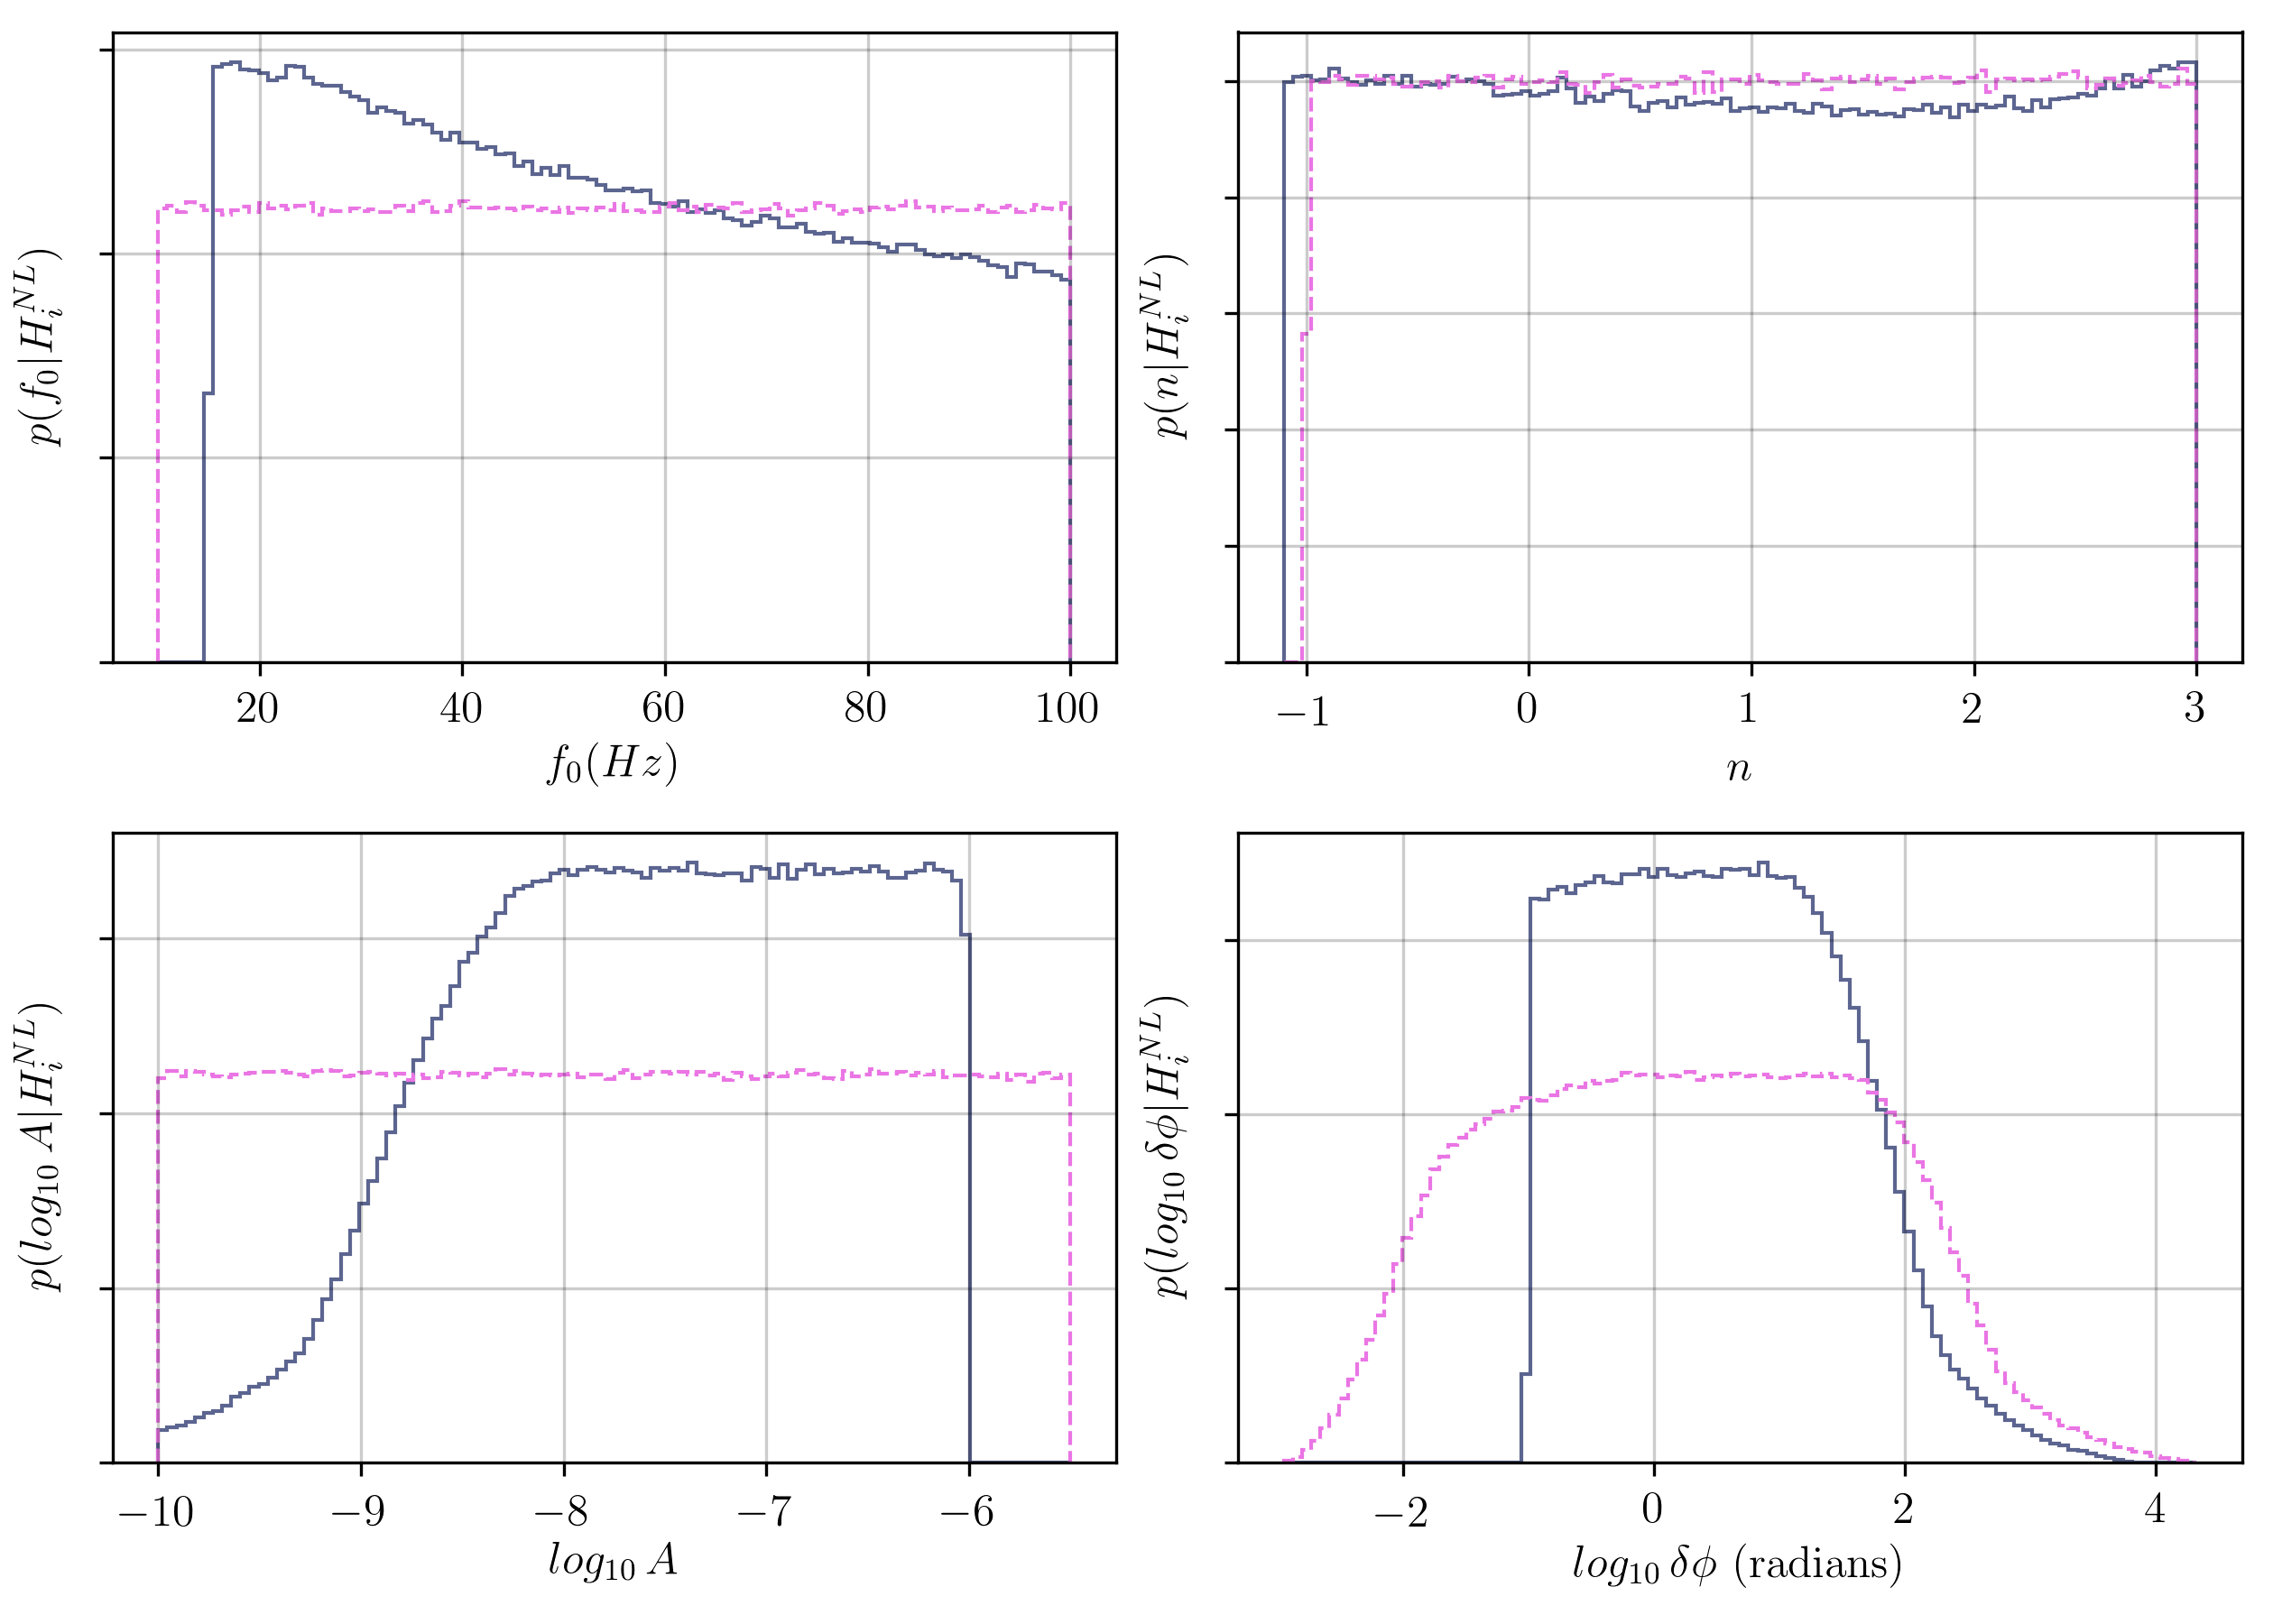
\includegraphics[width=0.9\columnwidth]{figs/chapter6/all_pg_priors}
\caption{Prior probability distributions on the parameters $(f_0, n, A)$ for the waveform model $\mathrm{H}^{\mathrm{NL}} = \mathrm{H}_\mathrm{TaylorF2+NL}$ and the resulting prior on the gravitational-wave phase shift $\delta\phi$ shift due to nonlinear tides. The dark blue, solid lines shows the priors when $f_0$ is drawn from a uniform distribution between $15$ and $100$~Hz with a $\delta\phi \ge 0.1$~rad constraint restricting some of the prior space. The pink, dotted lines represent prior distributions on the nonlinear tidal parameters similar to~\cite{abbott2019constraining}.}
\label{fig:priors}
\end{figure}

A stricter approach to constructing a prior distribution that considers $p$-$g$ mode effects that are distinguishable from standard waveforms is to examine the fitting factor between a distribution of $p$-$g$ mode waveforms and a set of comparable TaylorF2 waveforms. To do so, we examine the fitting factor of our Bayesian inference analysis with respect to a template bank of non-spinning, mass-only TaylorF2 waveforms. We construct a template bank of $\sim 20,000$ non-spinning, mass-only waveforms of comparable masses to the prior distribution on the mass parameters. The template bank is constructed with component masses, $m_{(1,2)} \in (1.0, 2.0) M_{\odot}$, chirp masses, $\mathcal{M}_c \in (1.1826, 1.2126) M_{\odot}$, and a minimal match placement of 99.9\%. We then place a threshold on the evidence calculation from the Bayesian analysis based on the maximum overlap with this template bank of standard waveforms. This permits an analysis of the Bayes factor for nonlinear tides where the prior distribution on $p$-$g$ mode parameters is determined by the fitting factor with a set of standard signals.

\section{Methods} \label{sec:methods}
We use the gravitational-wave strain data from the Advanced LIGO and Virgo detectors for the GW170817 event, made available through the GW Open Science Center~\citep{Vallisneri:2014vxa,gw170817-losc}. We then repeat the analysis of~\cite{de2018tidal} using the waveform model $H_\mathrm{TaylorF2+NL}$ to compute the evidence $p(\mathbf{d}\, | \, \mathrm{H}_\mathrm{TaylorF2+NL})$.

We use Bayesian model selection to determine which of the two waveform models described in Sec.~\ref{sec:waveform} is better supported by the observation of GW170817. Bayes theorem in Eq.~(\ref{eq:bayestheorem}) permits us a method for model  through the ratio of the evidence from each model. This ratio of the model evidences is called the Bayes factor, which we denote as $\mathcal{B}$. A Bayes factor greater than unity indicates support for the model in the numerator, while a Bayes factor less than unity indicates support for the model in the denominator. The Bayes factor can be written as,
\begin{equation}
\mathcal{B} = \frac{\mathcal{Z}\left(\mathbf{d}|H_\mathrm{TaylorF2+NL}\right)}{\mathcal{Z}\left(\mathbf{d}|H_\mathrm{TaylorF2}\right)}.
\label{eq:bayesfactor}
\end{equation}
The numerator of Eq.~(\ref{eq:bayesfactor}) is the evidence for nonlinear tides $p\left(\mathbf{d}|H_\mathrm{TaylorF2+NL}\right)$. For the denominator of Eq.~(\ref{eq:bayesfactor}), we use the evidence $\mathcal{Z}(\mathbf{d}|H_\mathrm{TaylorF2})$ provided as supplemental materials by~\citep{de2018tidal}.

Posterior distributions for parameters of interest can be also computed by marginalizing the posterior probability distribution over other parameters.  Marginalization to obtain the posterior probabilities and the evidence is performed using Markov Chain Monte Carlo (MCMC) techniques. To compute posterior probability distributions and evidences, we use the \emph{PyCBC Inference} software~\citep{alex_nitz_2018_1208115,biwer2019pycbc} using the parallel-tempered \emph{emcee} sampler~\citep{emcee,vousden:2016}.
This sampler allows the use of multiple temperatures to sample the parameter space~\citep{emcee, doi:10.1143/PTPS.157.317, B509983H}. These multiple temperatures $\beta$ permit the construction of tempered posterior distributions that form a slow thermodynamic transition from the prior distribution to the posterior distribution in Eq.~\ref{eq:bayestheorem}. Tempered posteriors are called power-posteriors in~\cite{lartillot2006computing, friel2008marginal}. The power-posterior can be according to:
\begin{equation}
    \mathcal{P}\left(\vec{\theta}|\mathbf{d}, H\right)_\beta \propto \pi\left(\vec{\theta} | H\right) \mathcal{L}\left(\mathbf{d} | \vec{\theta}, H\right)^\beta.
\end{equation}\label{eq:power_posterior}
The normalization constant for a power-posterior is the evidence for that power-posterior, given as $\mathcal{Z}(\mathbf{d}|H)_\beta = \int \pi\left(\vec{\theta} | H\right) \mathcal{L}\left(\mathbf{d} | \vec{\theta}, H\right)^\beta d\vec{\theta}$.

From these power-posterior distributions we use the thermodynamic integration method~\citep{lartillot2006computing,friel2008marginal} to estimate the logarithm of the evidence, ln $\mathcal{Z}$, given as:
\begin{equation}
\textrm{ln} \, \mathcal{Z} = \int_0^1 \langle \textrm{ln} \, \mathcal{L} \rangle_{\beta} \, d\beta.
\label{eq:thermoint}
\end{equation}
We provide a more thorough derivation in Appendix~\ref{sec:ti_ss_method_derivation}. The estimate of the evidence is determined by the integral over inverse temperatures, $\beta$, of the average untempered log likelihood, $\langle \textrm{ln}\, \mathcal{L} \rangle_{\beta}$, drawn from the power-posterior corresponding to the inverse temperature $\beta$. An approximation to this integral can be made through use of trapezoid rule integration method. Following~\cite{de2018tidal} we use $51$ temperatures where we use a combination of geometric and logarithmic temperature placements to improve the accuracy of the integral~\citep{liu2016evaluating}.

We verify the results of the thermodynamic integration evidence calculation by comparing it with the steppingstone algorithm~\citep{xie2010improving}, which utilizes the same likelihoods from multi-tempering sampling as the thermodynamic integration method. Both trapezoidal rule thermodynamic integration and steppingstone methods can have some bias in the estimate of the logarithm of the Bayesian evidence due to a finite number of temperatures being used. This bias is mitigated by an increased number of temperatures~\citep{xie2010improving, Russel:2018pqv}. Additionally, this bias can be mitigated in thermodynamic integration by improving the order of the quadrature integration~\citep{friel2014improving}. We also use a higher order trapezoidal rule from~\cite{friel2014improving} and verify that the results are consistent.

We also estimate the error for each method of evidence calculation. The thermodynamic integration method and steppingstone algorithm both contain Monte Carlo error~\citep{annis2019thermodynamic}. For the thermodynamic integration method the Monte Carlo error on the thermodynamic integral can be estimated following the methodology of~\cite{annis2019thermodynamic}. We use this same uncertainty estimate for the higher order trapezoidal rule as well. In~\cite{xie2010improving} there is a Monte Carlo variance estimate for the logarithm of the evidence from the steppingstone method that we also use here.

The last source of error in the evidence calculation that we consider is whether the MCMC has converged to stable likelihood values across all of the temperatures. This requires examining the stability of the evidence calculations as the MCMC progresses. Independent samples are drawn according to the $\mathrm{n_{acl}}$ method as described by~\cite{biwer2019pycbc} at various points in the run. This method takes a specific endpoint iteration, takes half the endpoint iteration as the starting point iteration, and calculates the autocorrelation length of the samples between the starting point and the endpoint iteration. Independent samples are drawn in intervals of the maximum autocorrelation length for the samples within this segment. We divide the full run into $12$ segments and calculate the evidence from each one of these segments to examine how the evidence progresses along the MCMC iterations. Gradually the evidence begins to settle towards a constant value as the MCMC progresses. We take the difference between the last two evidence estimates as the convergence error.

We estimate the total error on our evidence calculations, $\sigma_{\mathrm{ln} \, \mathcal{Z}}$, by adding the errors in quadrature according to,
\begin{equation}
\sigma_{\mathrm{ln} \, \mathcal{Z}} = \sqrt{ \sigma_{\mathrm{MC}}^2 + \sigma_{\mathrm{convergence}}^2 } \, .
\label{eq:errorprop}
\end{equation}
Here, the error $\sigma_{MC}$ is the Monte Carlo error and $\sigma_{\mathrm{convergence}}$ is the convergence error. Finally, to estimate the Bayes factors we model the log evidence as a normal distribution, with mean given from the log evidence calculation, and standard deviation given by the error propagation formula in Eq.~(\ref{eq:errorprop}). The logarithm of the Bayes factor can then be calculated from the difference in the logarithm of the evidences. The standard Bayes factor is then the exponential of the logarithm of the Bayes factor.

As a means of verifying the results from the above Bayes factor calculations we also make use of the Savage-Dickey density ratio method~\citep{edwards1963bayesian, dickey1971weighted, wagenmakers2010bayesian} for calculating the Bayes factor of the model where the $p$-$g$ mode parameters were chosen independently of one another. This is the approach taken in~\cite{abbott2019constraining}.

For certain kinds nested models where prior distributions on parameters are \textit{factorizable}, or independent from one another, there exists a method for deriving the Bayes factor for two models from one parameter estimation analysis. If there exists a parameter $X$ for which at a critical value $X_\mathrm{crit}$ the parameter model is equivalent to a nested model that has no parameterization in $X$, then the Bayes factor for the model with $X$ relative to the model without $X$ is taken as the limit of the prior density at $X_\mathrm{crit}$ relative to the posterior density at $X_\mathrm{crit}$. This method does not require a multi-dimensional integral to be approximated, but only requires the likelihood ratio of the prior density and posterior density at $X_\mathrm{crit}$.  In the case of the $p$-$g$ mode instability the parameter that effectively turns-on-and-turns-off the instability is the amplitude factor $A$. We can in effect evaluate the ratio between the prior distribution density as $A \to 0$ and the posterior distribution density as $A \to 0$. This expression thus can be written as:
\begin{equation}\label{eq:sddr_bayes_factor}
    \mathcal{B}^{\mathrm{NL} \, \,}_{\, \, !\mathrm{NL}} = \lim_{\mathrm{A} \to 0} \, \frac{\pi\left(\mathrm{A} | H^{NL}\right)}{\mathcal{P}\left(\mathrm{A} | \mathbf{d}, H^{NL}\right)}.
\end{equation}
Formally, the parameter model is constructed such that the prior density on $A$ is distributed uniformly in $\mathrm{log}_{10} \, A$ and so the limit cannot be strictly taken from within the data acquired in these analyses. However, when $A is 10^{-10}$, the matched-filter is not sensitive in this data set to distinguish the difference between $A=0$ to $> 99.999\%$ overlap, indicating that the substituting $A \to 0$ for $A \to 10^{-10}$ will likely generate identical results. We provide a more rigorous introduction and derivation for the Savage-Dickey density ratio method in Appendix~\ref{sec:sddr_derivation}.

This changes the problem of inference from one-dimensional numerical integration to probability density inference. In our case, we only have one model that has a prior on $A$ that is independent of all of the other priors and so we focus on the model that is most like \cite{abbott2019constraining}, where $A$ is uniform in $\log_{10}$ between $10^{-10}$ and $10^{-5.5}$. Fortunately, the prior distributional density is analytically known to us at $10^{-10}$, and so we only need to infer the probability density of the posterior distribution at $10^{-10}$. There are a variety of methods for estimating the density of a probability distribution when the distribution has to be constructed from sampled data. The simplest method is to construct histograms or use a kernel density function. In  ~\cite{wagenmakers2010bayesian} it is recommended that the logspline-density package in R be used~\citep{stone1997polynomial}. We make use of two histogram methods~\citep{scott1979optimal, Freedman1981}, a Gaussian kernel density estimator with boundary-bias corrections~\citep{lewis2015getdist}, and a logspline-density-estimator. We find the Bayes factors they all estimate to be consistent with those found with the multi-tempered Bayes factor estimators. We more fully describe the methods in Appendix~\ref{sec:prob_density_estimator}.

\section{Results}
\label{sec:results}
Compared to the standard waveform mode, we find that the $p$-$g$ mode model with priors where $\delta \phi$ is unconstrained gives a Bayes factor of order unity. When we use $p$-$g$ mode priors where $\delta \phi$ $>$ $0.1$~radians we also find a Bayes factor of order unity. Following the Bayes factor interpretation of \cite{kass1995bayes, jeffreys1998theory}, these Bayes factors cannot be considered to be statistically significant. A Bayes factor of unity indicates that whatever prior beliefs we had about the plausibility of the $p$-$g$ mode instability prior to GW170817 is unchanged by the observation of GW170817. For the narrow range of $15 \le f_0 \le 100$~Hz where $\delta \phi > 0.1$~rad, we find that the Bayes factors are $\mathcal{B} \sim 0.7$. This is also true of the prior range $10 \le f_0 \le 100$~Hz with unconstrained $\delta \phi$. The broader range  $15 \le f_0 \le 800$~Hz, where $\delta \phi > 0.1$~rad, we find that $\mathcal{B} \sim 0.7$ as well. Our estimated statistical error on Bayes factors due to Monte Carlo error and convergence error is $\sim \pm 0.1$ at the $90$\% confidence level. We enumerate the specific results of the multi-tempered evidence estimators in subsection~\ref{sec:ti_ssa_performance} and for the unconstrained $\delta \phi$ prior distribution we verify the results of these multi-tempered estimates with the Savage-Dickey density ratio test in subsection~\ref{sec:prob_density_estimator_performance} 

\subsection{Multi-Tempered Evidence Estimates}\label{sec:ti_ssa_performance}
Using the stuff from earlier chapter we can see the distributions of the logarithm of the evidence for the astrophysical hypothesis on $p$-$g$ mode instability for the unconstrained $\delta \phi$ prior in Fig.~\ref{fig:lvc_sim_log_evidence_distr}.

\begin{figure}[th]
\centering
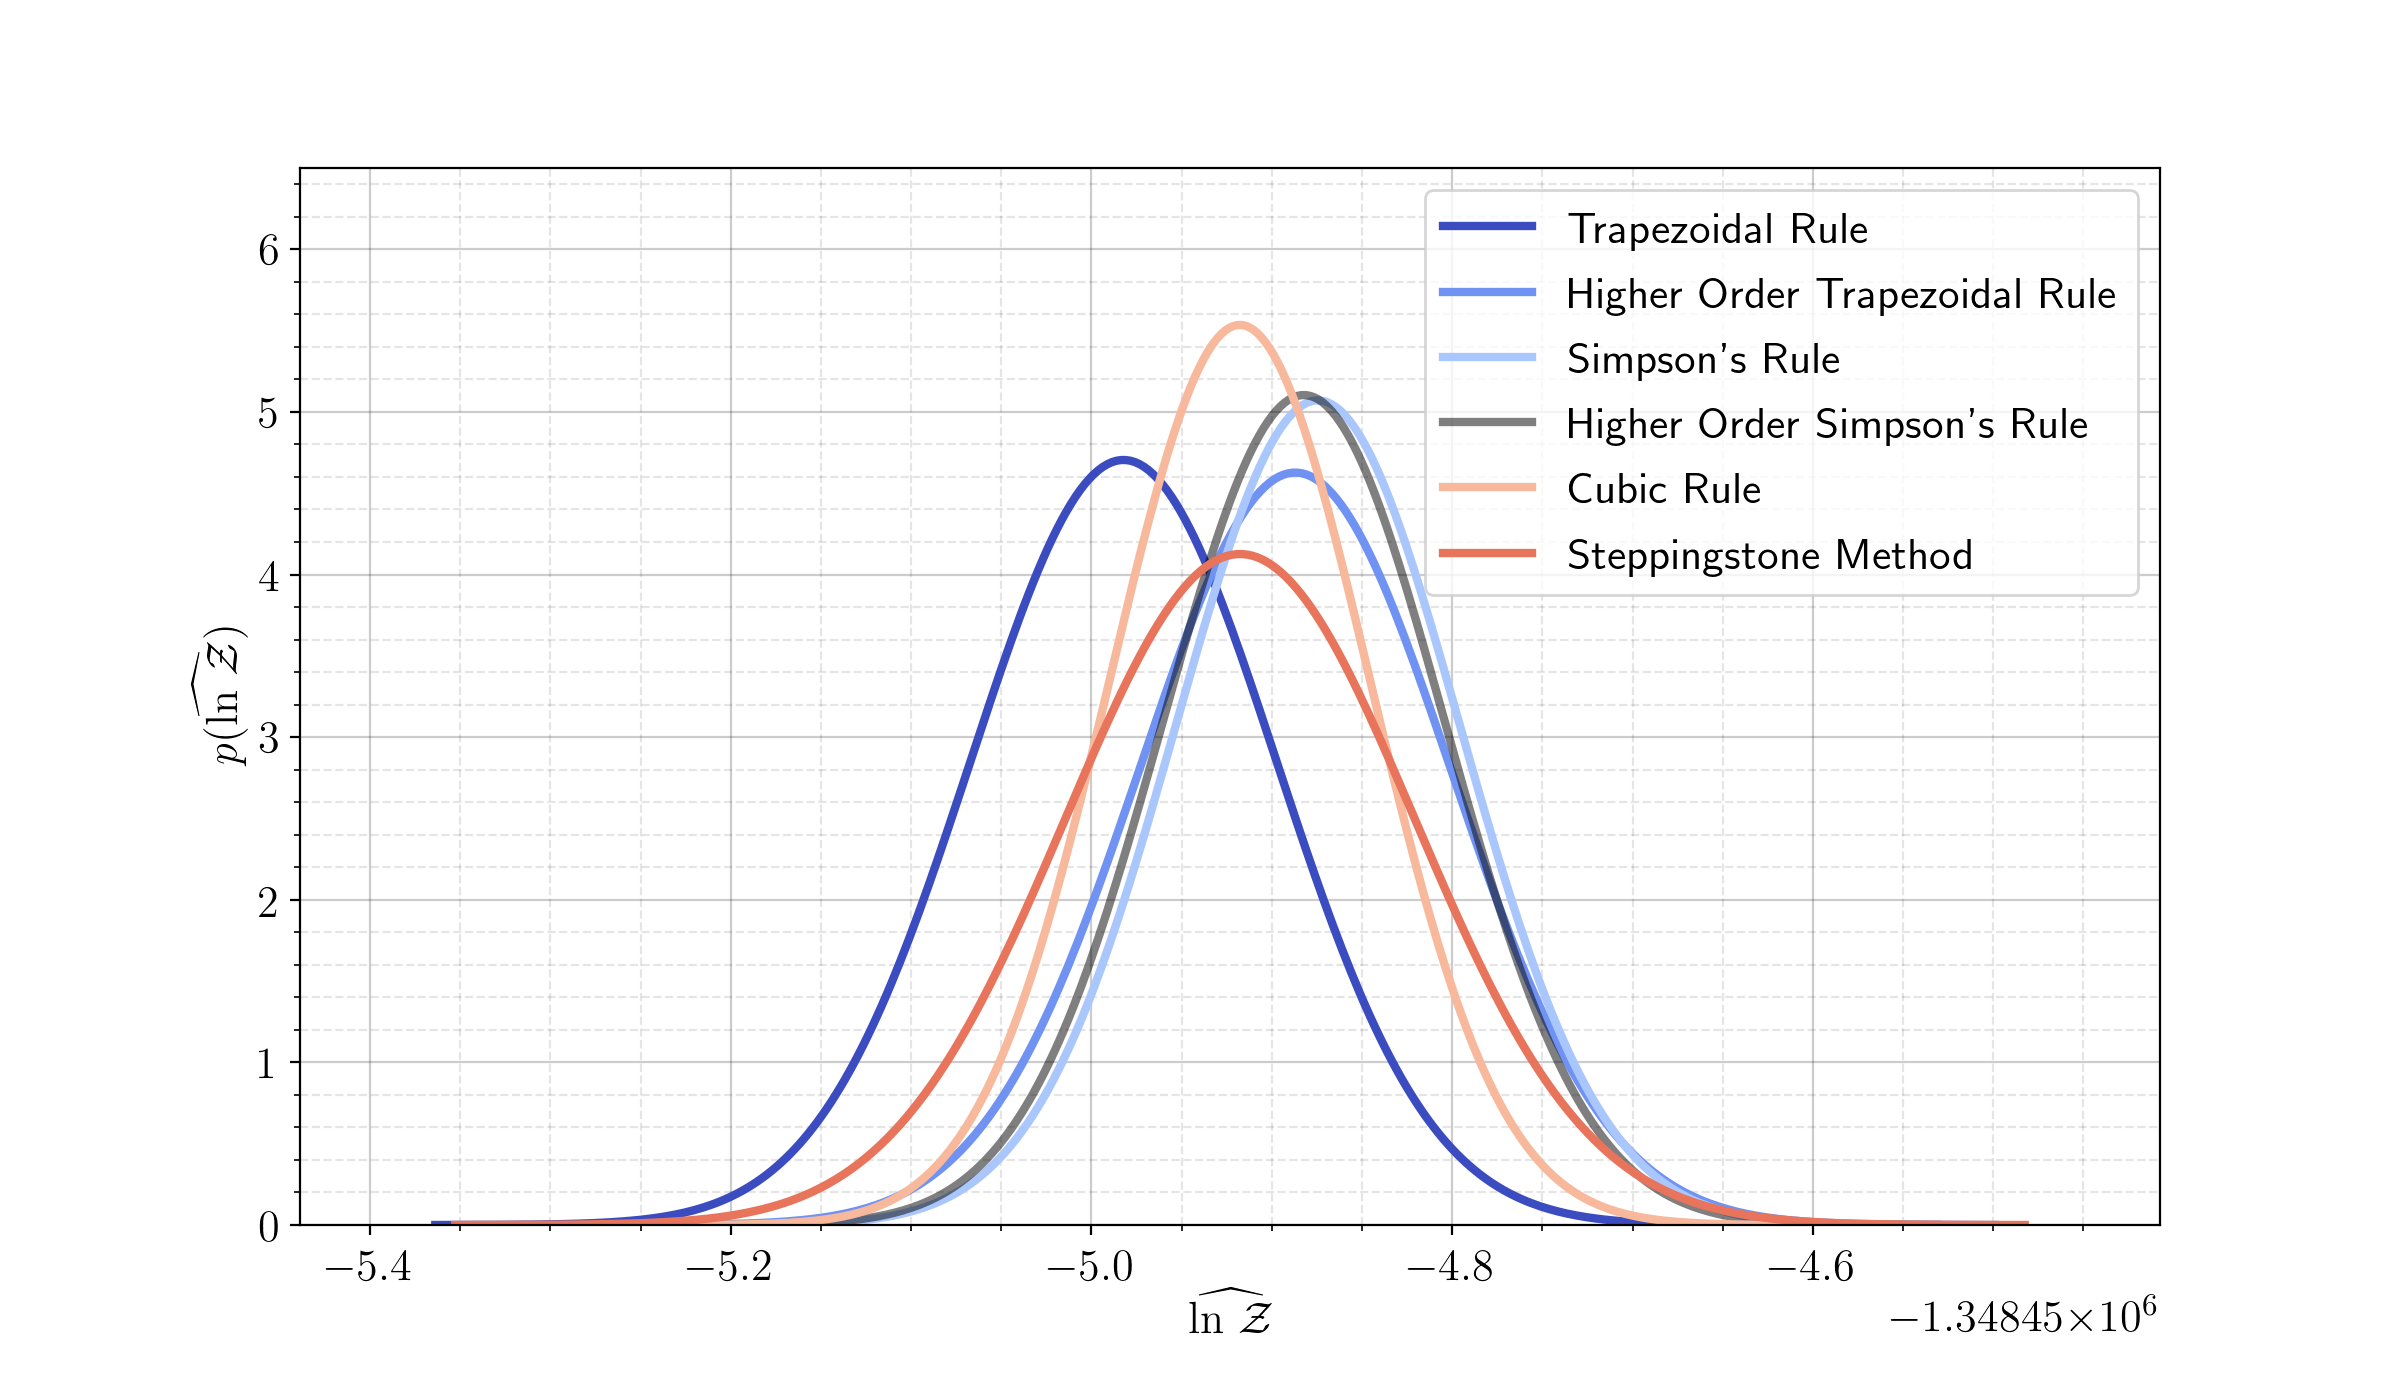
\includegraphics[width=1.0\textwidth]{figs/chapter6/multi_temper_log_z_lsc_sim.png}
\caption{The estimates of the logarithm of the evidence from multi-temper evidence integration methods. We model the logarithm of the evidence as a Gaussian in log-space. These data are for the logarithm of the evidence from the unconstrained $\delta \phi$ prior for the $p$-$g$ mode instability model. The trapezoidal rule estimates the lowest log evidence for this model, and the cubic rule has the smallest estimated statistical error uncertainty (the smallest confidence interval). The mean values of the higher order quadrature rules appear to be closer together to one another than they are to the trapezoidal rule.}
\label{fig:lvc_sim_log_evidence_distr}
\end{figure}

The logarithm of the Bayes factor is the difference of the logarithm of the evidence for one hypothesis and the logarithm of the evidence for another hypothesis:
\begin{equation}\label{eqn:log_bayes_factor}
    \mathrm{ln} \, \mathcal{B}^A_B = \mathrm{ln} \, \mathcal{Z}_{\mathrm{A}} - \mathrm{ln} \, \mathcal{Z}_{\mathrm{B}}
\end{equation}
However, since we treat $\mathrm{ln} \, \mathcal{Z}_{\mathrm{A}}$ as a random variable who's true value is unknown and so we must deal with the uncertainty in $\widehat{\mathrm{ln} \, \mathcal{Z}_{\mathrm{A}}}$. The logarithm of the Bayes factor then becomes the difference between two probability distribution functions. This can be solved via convolution and has been solved for the Gaussian case~\citep{bromiley2003products}. Thus the resultant $\widehat{\mathrm{ln} \, \mathcal{B}^A_B}$ is itself a Gaussian distribution function with mean $\mu_{\widehat{\mathrm{ln} \, \mathcal{B}^A_B}} = \mu_{\widehat{\mathrm{ln} \, \mathcal{Z}_A}} - \mu_{\widehat{\mathrm{ln} \, \mathcal{Z}_B}}$ and standard deviation $\sigma_{\widehat{\mathrm{ln} \, \mathcal{B}^A_B}} = \sqrt{\sigma_{\widehat{\mathrm{ln} \, \mathcal{Z}_A}}^2 + \sigma_{\widehat{\mathrm{ln} \, \mathcal{Z}_B}}^2 }$~\citep{bromiley2003products}. This thus gives us the following expression for the distribution function that describes our uncertainty on the logarithm of the Bayes factor:
\begin{equation}\label{eqn:p_log_b}
    p(\widehat{\mathrm{ln} \, \mathcal{B}^A_B}) = \left(\frac{1}{\sqrt{2 \pi \sigma_{\widehat{\mathrm{ln} \, \mathcal{B}^A_B}}}} \right) \mathrm{exp} \left \{-\frac{\left(\widehat{\mathrm{ln} \, \mathcal{B}^A_B} - \mu_{\widehat{\mathrm{ln} \, \mathcal{B}^A_B})}\right)^2} {2 \sigma^2_{\widehat{\mathrm{ln} \, \mathcal{B}^A_B}}}  \right\}.
\end{equation}

The expression in Eq.~(\ref{eqn:p_log_b}) is a Gaussian distribution function in $\widehat{\mathrm{ln} \, \mathcal{B}^A_B}$, but we often prefer to know the estimate on $\mathcal{B}^A_B$ and so we must transform coordinates. This transformation of coordinates, fortunately, is a well-known distribution called the log-normal distribution and it is able to be described in terms of the coordinates used in Eq.~(\ref{eqn:p_log_b}). Below we write out our log-normal probability distribution function for $\widehat{\mathcal{B}^A_B}$:
\begin{equation}
    p(\widehat{\mathcal{B}^A_B}) = \frac{1}{\widehat{\mathcal{B}^A_B} \, \sigma_{\widehat{\mathrm{ln} \, \mathcal{B}^A_B}}} \frac{1}{2\pi} \mathrm{exp} \left \{-\frac{\left(\mathrm{ln} \, \widehat{\mathcal{B}^A_B} - \mu_{\widehat{\mathrm{ln} \, \mathcal{B}^A_B})}\right)^2} {2 \sigma^2_{\widehat{\mathrm{ln} \, \mathcal{B}^A_B}}}  \right\}.
\end{equation}
This is the implementation that we have used to represent that Bayes factor in this study. It is worth noting that for a sufficiently small standard deviation on the logarithm of the Bayes factor, the probability of the distribution function will look approximately Gaussian in shape. One useful property of the log-normal Bayes factor distribution is that the median of the log-normal Bayes factor distribution is identical to the point-estimate Bayes factor, $\mathcal{B}^A_B = \mathrm{exp} \left[\mathrm{ln} \, \mathcal{Z}_{\mathrm{A}} - \mathrm{ln} \, \mathcal{Z}_{\mathrm{B}} \right]$. Note, that the expectation value (mean) of $\mathcal{B}^A_B$ is always right-skewed of the median, while the mode of the distribution is left-skewed relative to the median. Large standard deviations on the logarithm of the evidence will create very long tails for the distribution of the Bayes factor, which can make decision-making on Bayes factors more risky. Future studies should consider limiting the error on the logarithm of the evidence to mitigate the larger error on the Bayes factor.

Our Bayes factor estimation from $6$ multi-tempered estimators on the logarithm of the Bayes factor can be seen in Fig.~\ref{fig:lvc_sim_uni_ceos_bayes_distr} when comparing the hypothesis on $p$-$g$ mode instability for the unconstrained $\delta \phi$ prior to the hypothesis presented in~\cite{de2018tidal} for the uniform mass prior with a common equation of state constraint. The different methods appear to give similar probability distributions on the Bayes factor. Those estimators with large standard deviations in $\mathrm{log} \, \mathcal{B}$ have tails that skew towards a Bayes factor of unity.


\begin{figure}[th]
\centering
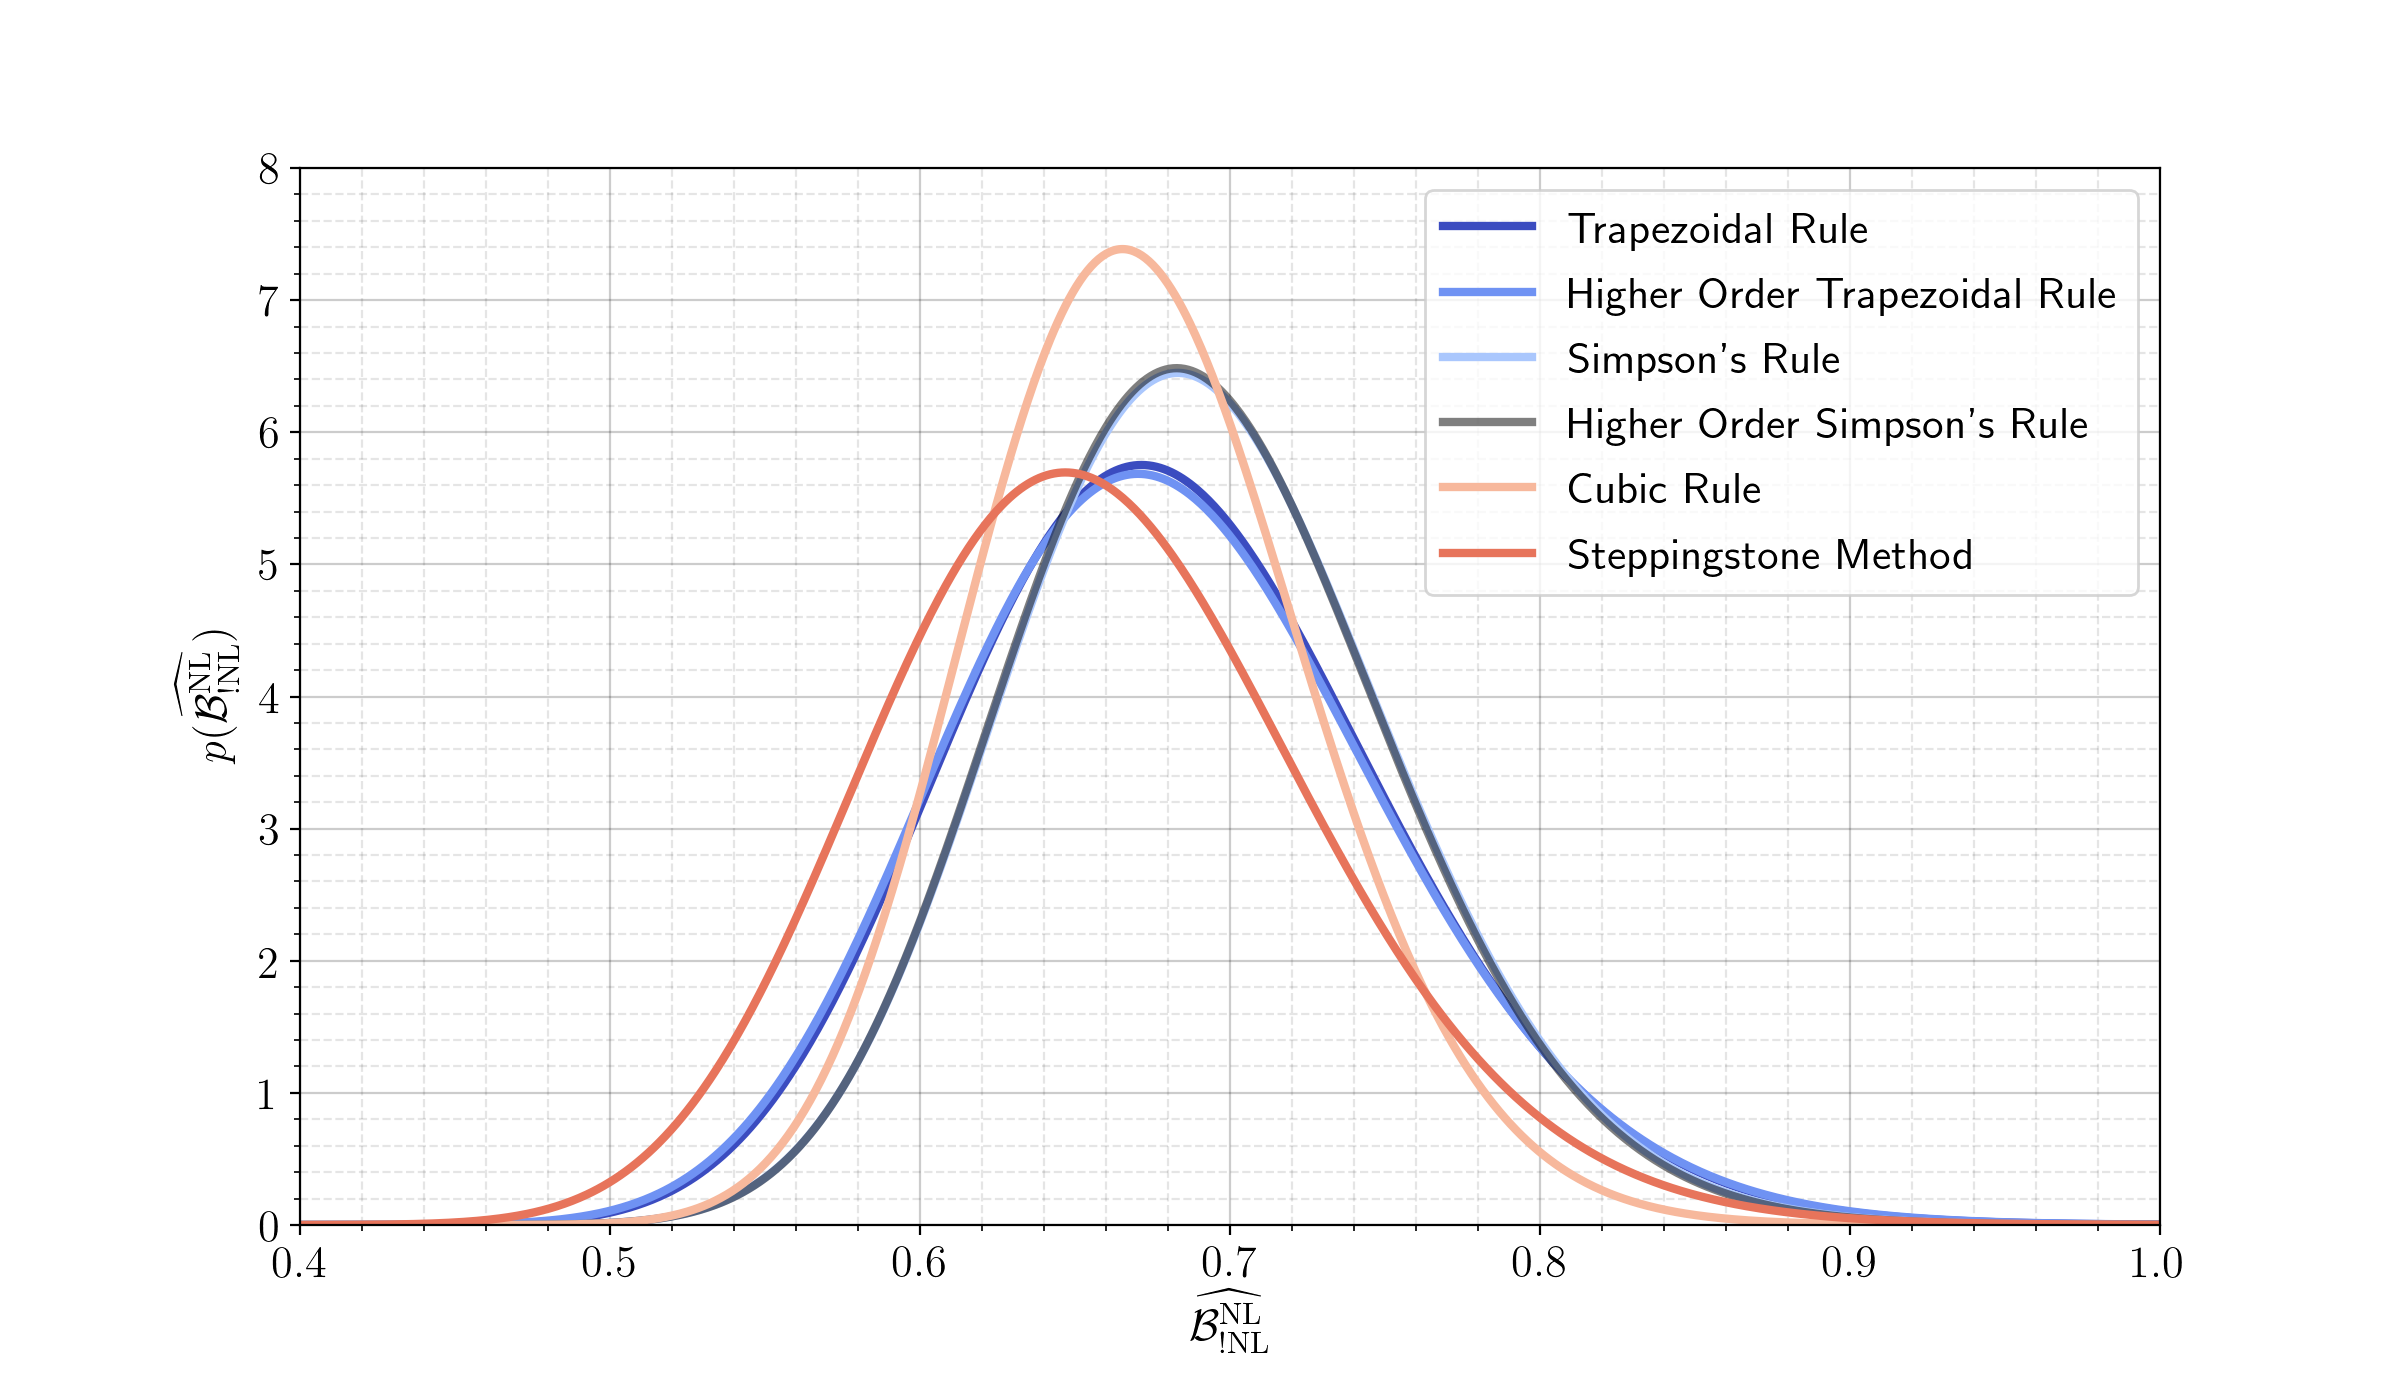
\includegraphics[width=1.0\textwidth]{figs/chapter6/multi_temper_bayes_lsc_sim_uni_ceos.png}
\caption{The distribution for the Bayes factor for nonlinear tides from $p$-$g$ mode instability from the unconstrained $\delta \phi$ prior relative to the uniform mass, common equation of state prior from~\cite{de2018tidal} under the assumption that the logarithm of the evidence for each model is well approximated by a Gaussian distribution.  but our method is sufficiently accurate in the high-sample limit. When the uncertainty on the logarithm of the evidences in the Bayes factor estimation are sufficiently small, the Bayes factor distribution is approximately normal in shape, but formally they are log-normal distributions.}
\label{fig:lvc_sim_uni_ceos_bayes_distr}
\end{figure}

The Bayes factors for all hypotheses using all of the multi-tempered methods can be seen in Table~\ref{table:Bayes}. The median values of the Bayes factors range between roughly $0.63$ and $0.76$, with the $5^{\mathrm{th}}$ and $95^{\mathrm{th}}$ percentile interval being  around $\pm 0.1$ with a skew towards Bayes factors of $1$. Under a binary choice between the $p$-$g$ mode instability model and the corresponding model without $p$-$g$ mode instability we can calculate a posterior probability of one choice over the other choice. Without giving preference to either model, we can calculate a posterior probability as $p^{\mathrm{NL}}_{\mathrm{!NL}}$ = $\mathcal{B}^{\mathrm{NL}}_{\mathrm{!NL}} / ( 1 + \mathcal{B}^{\mathrm{NL}}_{\mathrm{!NL}})$. Thus, the Bayes factor of $0.63$ corresponds to a posterior probability of $39$ \%  and a Bayes factor of $0.76$ corresponds to a posterior probability of $43$ \%. If we consider the $\pm$ 0.1 ends of the Bayes factor estimation, a Bayes factor of $0.53$ can be interpreted as a posterior probability of $34$\% probability, while a Bayes factor of $0.86$ can be interpreted as the model having a $46$ \% posterior probability. If we consider all models collectively, the posterior probability on any one, particular model reduces significantly.

\subsection{Savage-Dickey Density Ratio Bayes Factors}\label{sec:prob_density_estimator_performance}
Below we report on the Savage-Dickey density test for finding the Bayes factor of the  on $p$-$g$ mode instability for the unconstrained $\delta \phi$ prior compared to a null-hypothesis, that is a hypothesis where $p$-$g$ mode instability is not modeled. Formally, this is the model presented in~\cite{de2018tidal} for the uniform mass prior with a common equation of state constraint however the Savage-Dickey density test makes no use of the data from~\cite{de2018tidal}. While this may sound somewhat outrageous, we will find that the results generally agree with those found using multi-tempered model selection techniques. The results of all of the Savage-Dickey density tests are collected and summarized in Table~\ref{table:Bayes_sddr}.

\subsection{Histogram Method}
An elementary method for estimating the probability density function is to histogram the samples and normalize the histogram to integrate to unity. Under this methodology the only relevant parameter to fitting the histogram to the data is the choice of bin-width, sometimes called bandwidth.

Two methods that we have used to try to maximize the fit of the histogram to the data are through the choice of plug-in bin-width algorithms. The algorithms are designed to minimize the error to the histogram density fit to an underlying density function. The first is Scott's rule~\citep{scott1979optimal} and is considered optimal relative to a density function that is normally distributed. The bin-width $h$ for this rule is defined as:
\begin{equation}
    h = \frac{3.5 \, \sigma}{N^{1/3}}.
\end{equation}
Here $\sigma$ represents the sample standard deviation of the data, and $N$ represents the number of samples in the data.

The second method is described in ~\cite{Freedman1981} and makes use of the interquartile range (IQR). The IQR is the difference between the $75^{\mathrm{th}}$ and $25^{\mathrm{th}}$ percentile of the data. The Freedman-Diaconis bin method ~\citep{Freedman1981}, where the bin-width $h$ is:
\begin{equation}
    h = \frac{2 \, \mathrm{IQR}}{N^{1/3}}
\end{equation}
Here $N$ represents the number of samples in the data.

Since the marginal prior (posterior) distribution functions on $A$ are distributed logarithmically, it is convenient to do the density estimation in the variable $\tilde{X} \equiv \mathrm{log}_{10} \, A$. Under this change of variables the marginal prior distribution on $\tilde{X}$ is uniform between $\tilde{X}=-10$ and $\tilde{X}=-5.5$, hence the distribution function is constant over all values of $\tilde{X}$:
\begin{equation}
    \pi\left(\tilde{X}\right) = \frac{1}{\tilde{X}_{max} - \tilde{X}_{min}} = 0.2\overbar{2}, \qquad -10.0 \leq \tilde{X} \leq -5.5
\end{equation}

Using the histogram bin-width rules from above we estimate the marginal posterior probability density at $\tilde{X} = -10.0$. To estimate a confidence interval on the Bayes factor from this method, we resample the the marginal posterior probability density distribution of $\mathrm{log}_{10} \, A$ via bootstrap method \cite{efron1992bootstrap} $5,000$ times. This gives us $5,000$ estimates of the Bayes factor and thus a distribution of possible Bayes factor values from this method. We find a $\mathcal{B}^{\mathrm{NL}}_{!\mathrm{NL}} = 0.66^{+0.08}_{-0.07}$ at the $90\%$ confidence interval for Scott's Rule and a $\mathcal{B}^{\mathrm{NL}}_{!\mathrm{NL}} = 0.66^{+0.08}_{-0.06}$ at the $90\%$ confidence interval for the Freedman-Diaconis Rule. For a comparison of the density estimates for the marginal posterior probability density on $\mathrm{log}_{10} \, A$ see Fig.~\ref{fig:density_estimators}. The Bayes factor uncertainty distribution is shown, in comparison to the other density estimators and the thermodynamic integration method uner the higher-order trapezoidal rule, in Fig.~\ref{fig:sddr_bayes_factor_comparisons}.

\subsection{Gaussian Kernel Density Estimator}
We use a Gaussian kernel density estimator available in the Python package GetDist~\citep{lewis2015getdist}. GetDist is a Python package intended to accurately estimate the underlying one-dimensional and two-dimensional posterior probability distribution functions from a Bayesian MCMC analysis. A rough understanding of a Gaussian kernel density estimator is that it uses small truncated-Gaussian distributions centered at samples of the data and combines the sum of the distributions into a smooth probability distribution function.

The advantage that GetDist offers over other Gaussian kernel density estimators is that it comes with robust linear-boundary bias correction to the standard Gaussian kernel density estimator. Sharp boundaries on the distribution function can cause bias to the probability distribution function estimation for Gaussian kernel density estimators~\citep{lewis2015getdist}, and the Savage-Dickey density ratio method in this application requires us to know the density of the posterior distribution at the boundary of the distribution. There are additional bias-correction and bandwidth optimization algorithms in the routine that help improve the accuracy of the density estimation. See~\cite{lewis2015getdist} for the full details.

We follow the same procedure in estimating the posterior probability density of $A$ at $10^{-10}$ as in the histogram method. We resample the posterior distribution through the bootstrap method to generate $5,000$ estimates of $\mathcal{P}(A =10^{-10}|\mathbf{d})$. This then yields an estimate of the Bayes factor at the $90\%$ confidence level of $\mathcal{B}^{\mathrm{NL}}_{!\mathrm{NL}} = 0.66^{+0.13}_{-0.1}$. For a comparison of the density estimates for the marginal posterior probability density on $\mathrm{log}_{10} \, A$ see Fig.~\ref{fig:density_estimators}. The Bayes factor uncertainty distribution is shown, in comparison to the other density estimators and the thermodynamic integration method under the higher-order trapezoidal rule, in Fig.~\ref{fig:sddr_bayes_factor_comparisons}.

\subsection{Logspline Density Estimator}
In the logspline density estimator of~\cite{stone1997polynomial} a univariate log-probability density is modeled by a cubic spline. The algorithm places knots of a cubic spline in an algorithmic fashion and uses an internal likelihood function to find a maximum likelihood number of knots (and placement) to use. Internal to the software package is a Bayesian model-selection routine based on the Akaike Information Criterion (AIC)~\citep{akaike1981likelihood} and the Bayesian Information Criterion (BIC)~\citep{schwarz1978estimating} to both ensure goodness of fit and to avoid over-fitting to the data. The details of the procedure are sophisticated and beyond the scope of this study. We utilize the maximum likelihood fit to the probability distribution function from the packages' model selection routine. We note that using the maximum likelihood fit is not very risky as the likelihood for other values of knot and knot placement as given from the package's fit routine provide posterior density estimates that are almost identical to the maximum likelihood fit.

We use the same bootstrap method outlined above to estimate the variability of the logspline algorithm relative to the variability of the data. We find an estimate of the Bayes factor at the $90\%$ confidence level of $\mathcal{B}^{\mathrm{NL}}_{!\mathrm{NL}} = 0.63^{+0.06}_{-0.05}$. For a comparison of the density estimates for the marginal posterior probability density on $\mathrm{log}_{10} \, A$ see Fig.~\ref{fig:density_estimators}. The Bayes factor uncertainty distribution is shown, in comparison to the other density estimators and the thermodynamic integration method under the higher-order trapezoidal rule, in Fig.~\ref{fig:sddr_bayes_factor_comparisons}.

\begin{figure}[th]
\centering
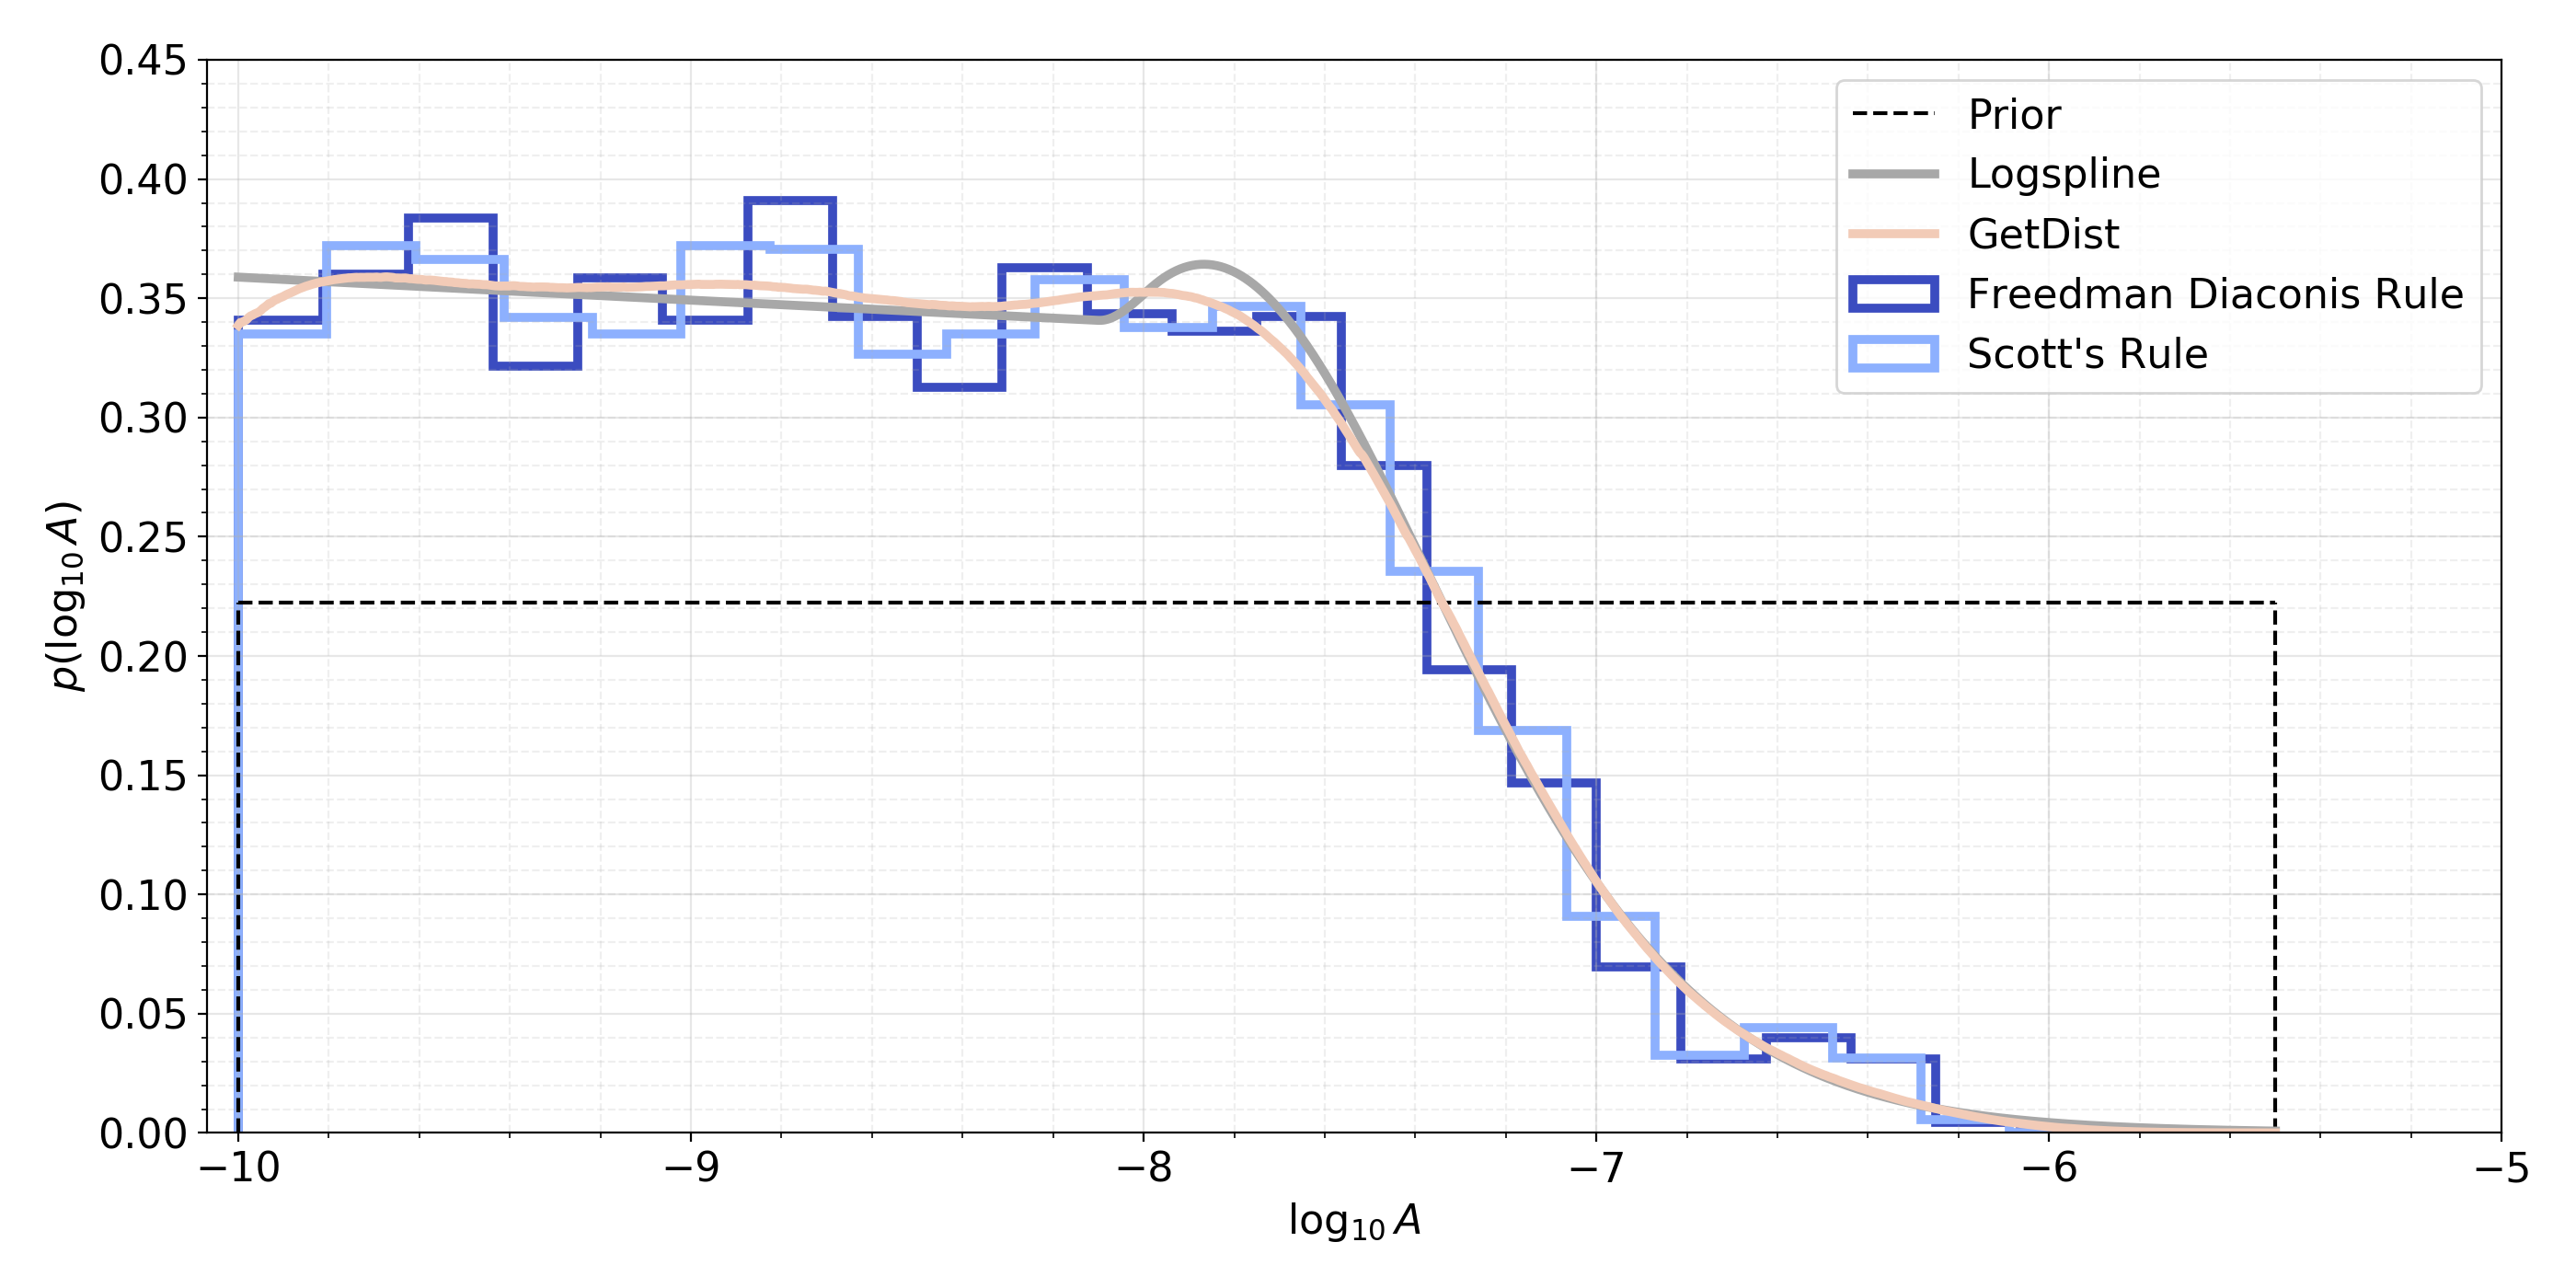
\includegraphics[width=1.0\textwidth]{figs/chapter6/prior_posterior_sddr.png}
\caption{The prior and posterior density estimations from different density estimators for the parameter $\mathrm{log}_{10} \, A$. The prior density is uniform in $\mathrm{log}_{10}$ and is $0.\overbar{2}$ between $-10$ and $-5.5$. The Logspline curve (dark grey) is the density estimation under the logspline density estimator. The GetDist (light pink curve) is the Gaussian kernel density estimator described in \cite{lewis2015getdist}. The histograms are FD and Scott for the Freedman-Diaconis binning rule and Scott's binning rule, respectively. We can see here that there is some wasted prior space at large $\mathrm{log}_{10} A$. Removing this low-likelihood region from the prior hypothesis model would likely move the $p$-$g$ mode instability Bayes factor closer to unity.}
\label{fig:density_estimators}
\end{figure}

\begin{figure}[th]
\centering
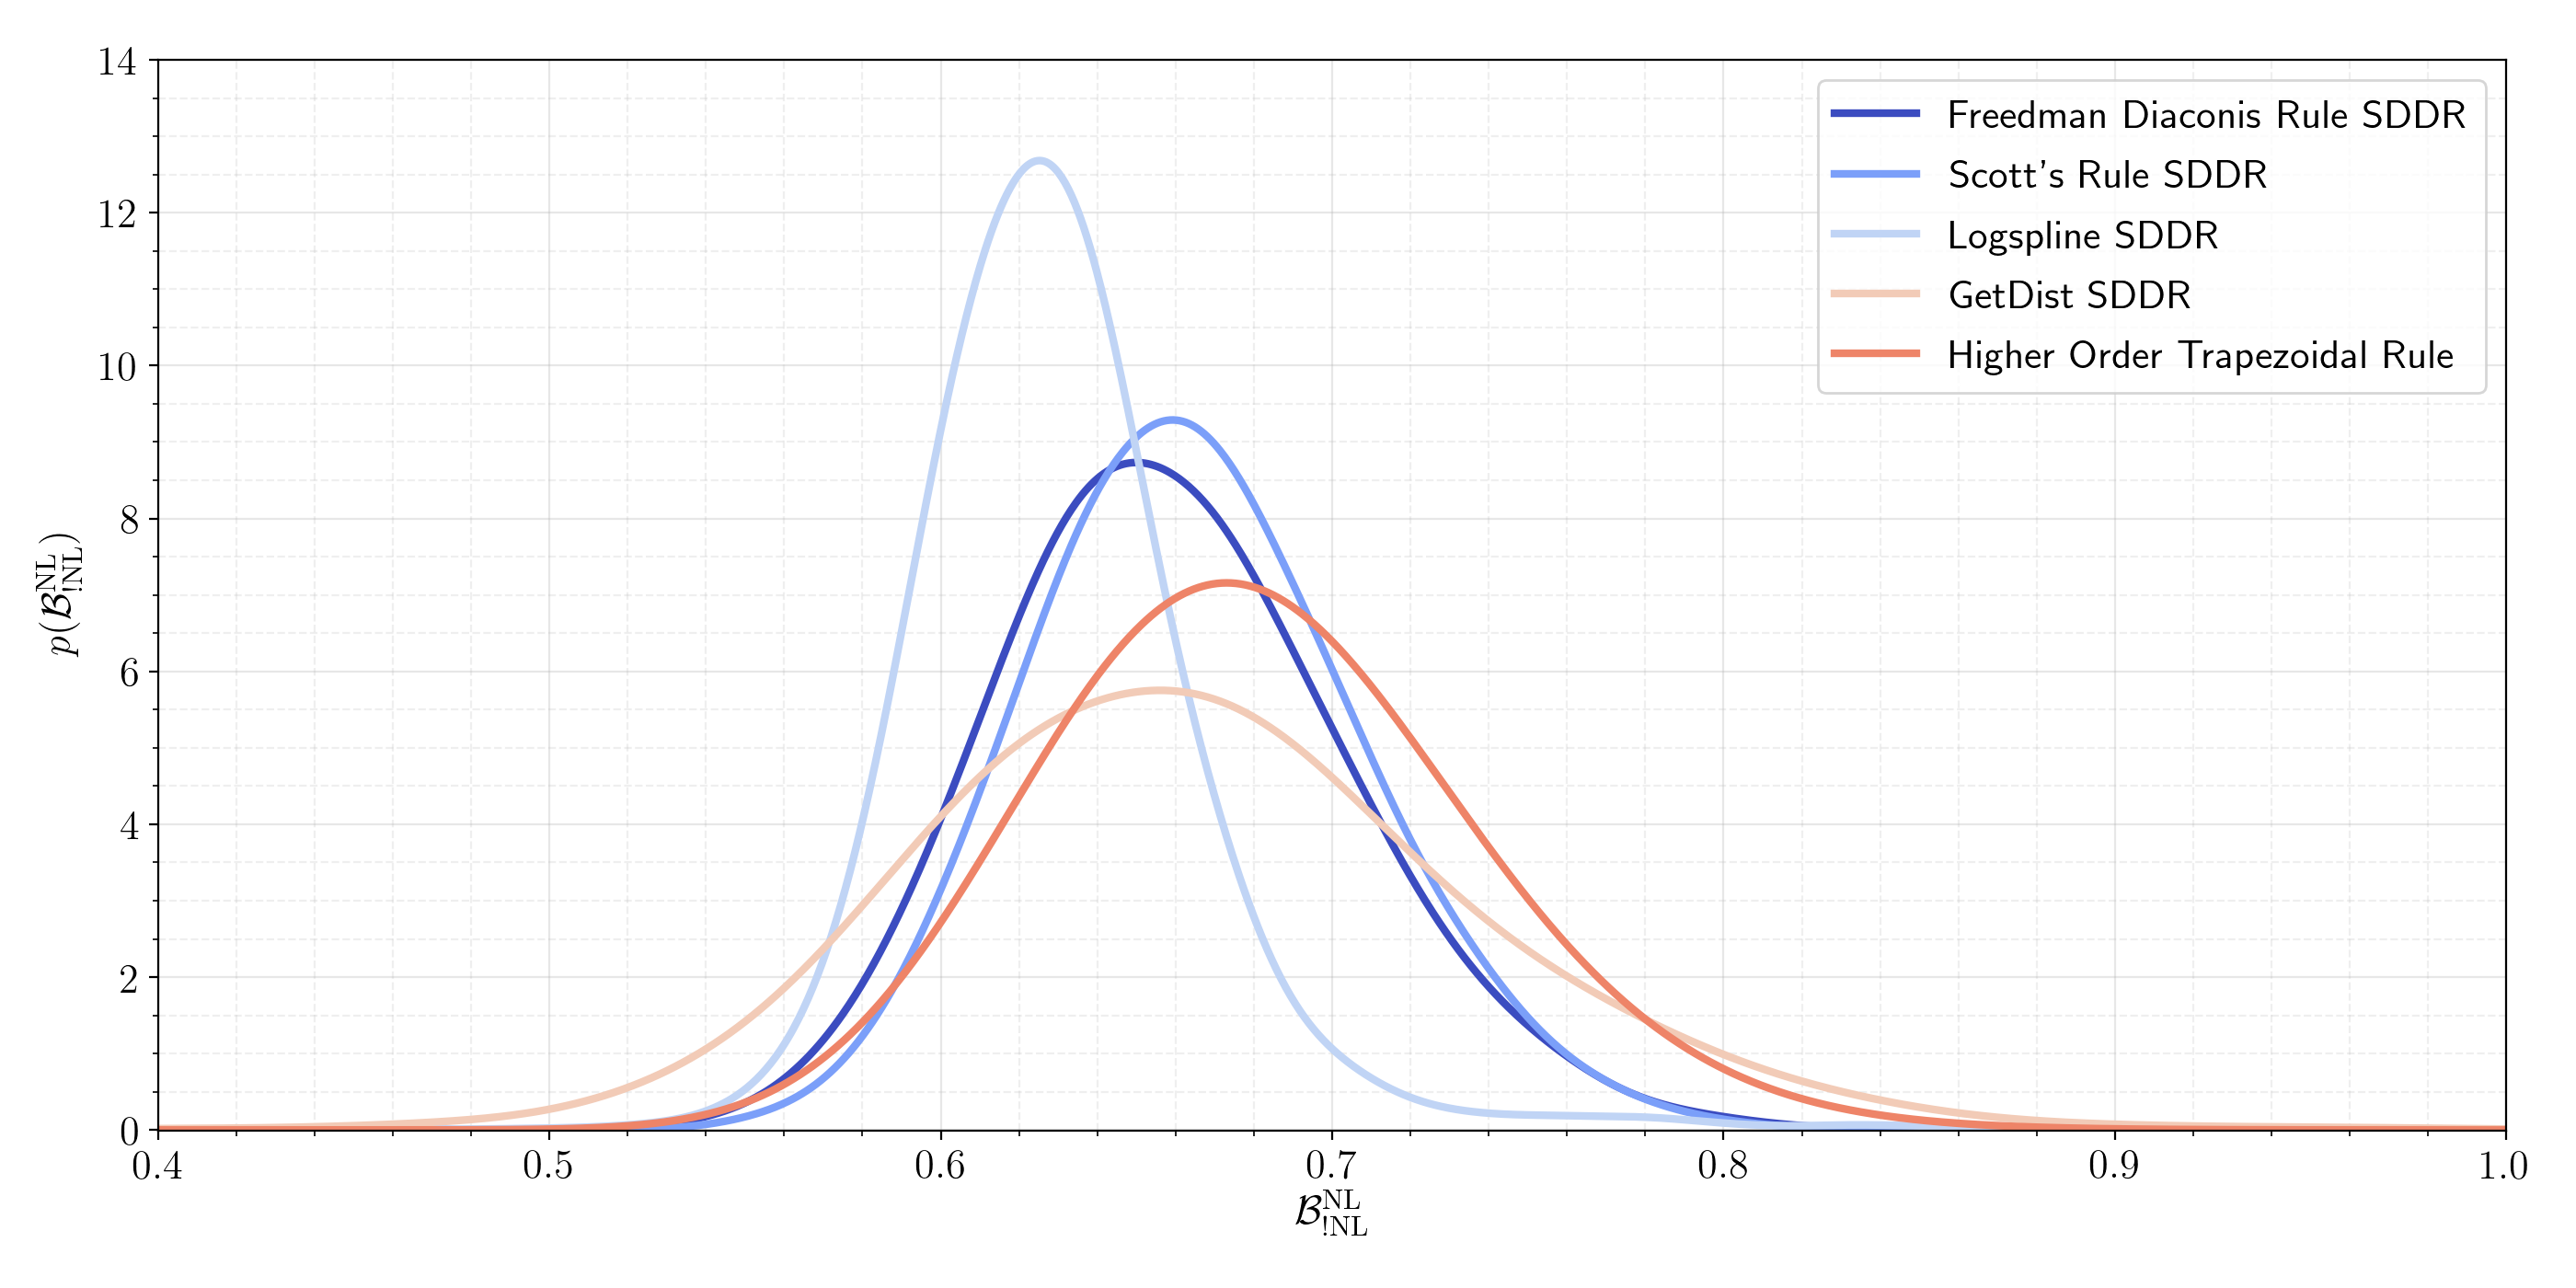
\includegraphics[width=1.0\textwidth]{figs/chapter6/sddr_bayes_factor.png}
\caption{A comparison of the Bayes factor estimates for $p$-$g$ mode instability with the permissive prior on $\delta \phi$ vs no $p$-$g$ mode instability from different methods. Here, SDDR refers to the Savage Dickey density ratio test for each corresponding estimator technique. We compare these results to the higher order trapezoidal rule from thermodynamic integration. The other multi-tempered Bayes factors are comparable to the one shown here and so are not displayed. The estimates generally agree as can be seen from comparing values in Table~\ref{table:Bayes} and Table~\ref{table:Bayes_sddr}.}
\label{fig:sddr_bayes_factor_comparisons}
\end{figure}


\subsection{Parameter Estimation Results}
When we consider the way that the nonlinear tides enter the Fourier phase in Eq.~(\ref{eqn:fourier_phase_eq1}), we see that if $n = 4/3$ then the nonlinear tides enter the Fourier phase of the waveform with the same power law dependence on frequency $f$ as the chirp mass, that is $\Psi(f) \propto f^{-5/3}$. We also note that for the effect of nonlinear tides to be degenerate with chirp mass, they must turn on at a frequency $f_0$ that is close to the low-frequency limit of the detector's sensitive band. If the effect turns on at higher frequencies, then the phasing will change in the detector's sensitive band and it is more difficult to compensate for the nonlinear tide effect with a change in chirp mass. 

The marginalized posterior distributions on parameters shown in Fig.~\ref{fig:uniform_f0_small} show a strong degeneracy between the source-frame chirp mass $\mathcal{M}^\textrm{src}$ and nonlinear tides that creates a tail in the chirp mass posterior skewed towards lower values of chirp mass than the value measured using the standard waveform model, $\mathcal{M}^\textrm{src} = 1.1867\pm0.0001\, M_\odot$~\citep{de2018tidal}. We see a peak in the posteriors of $n$ and $f_0$ at $n \lesssim 4/3$ and $f_0 \lesssim 35$~Hz. This parameter degeneracy is also correlated with large $A$, where $10^{-8} \lesssim A < 10^{-6}$. The samples with large posterior values of $\delta\phi$ seen in Fig.~\ref{fig:uniform_f0_small} are strongly correlated with source-frame chirp masses $\mathcal{M}^\textrm{src} \lesssim 1.1866.$ We have examined the change to the posterior distribution when changing the low-frequency cutoff of the likelihood integration from $20$~Hz to $25$~Hz, and to $30$~Hz. In these analyses, the peak in the posterior of $f_0$ tracks the low-frequency cutoff of the likelihood integration, confirming that this effect is due to the chirp-mass degeneracy with the low-frequency cutoff. The chirp mass degeneracy is also present in the analysis with the broader range of $f_0$, however it is not as pronounced in the posterior samples due to the larger prior space being explored. For the prior distributions discussed above, the observation of GW170817 does not provide strong statistical evidence either for or against the presence of nonlinear tides. 

\subsection{Can we improve the chirp mass measurement with an independent EM Observation?}
We noted in the introduction that we would require a strong constraint on the chirp mass independent of the gravitational wave data to mitigate the parameter degeneracy from the $p$-$g$ mode instability. Here we make a rough quantitative analysis of how tight an electromagnetic observation would have to constrain the chirp mass. To do so we must consider the joint posterior distribution, $\mathcal{P}(\mathcal{M} \, | \,  \mathbf{d_{GW}}, \mathbf{d_{EM}})$, from two statistically independent data sets, the gravitational wave data $\mathbf{d_{GW}}$, and a mock electromagnetic data set $\mathbf{d_{EM}}$. We must then define a (hyper) prior on the chirp mass that bridges the measured likelihood of the chirp mass for each data set to the posterior distribution. This expression looks as follows:
\begin{equation}
    \mathcal{P}(\mathcal{M} \, | \,  \mathbf{d_{GW}}, \mathbf{d_{EM}}) = \frac{\pi(\mathcal{M})}{\mathcal{Z}(\mathbf{d_{GW}}, \mathbf{d_{EM}})}  \,  \mathcal{L}(\mathbf{d_{GW}}, \mathbf{d_{EM}} \, | \, \mathcal{M}) = \frac{\pi(\mathcal{M})}{\mathcal{Z}(\mathbf{d_{GW}}, \mathbf{d_{EM}})} \, \mathcal{L}(\mathbf{d_{GW}} \, | \, \mathcal{M}) \, \mathcal{L}(\mathbf{d_{EM}} \, | \, \mathcal{M}).
\end{equation}
The separation of $\mathcal{L}(\mathbf{d_{GW}}, \mathbf{d_{EM}} \, | \, \mathcal{M}) = \mathcal{L}(\mathbf{d_{GW}} \, | \, \mathcal{M}) \, \mathcal{L}(\mathbf{d_{EM}} \, | \, \mathcal{M})$ follows from the two being statistically independent measurements of the chirp mass of GW170817. Here, $\mathcal{Z}(\mathbf{d_{GW}}, \mathbf{d_{EM}})$ is the normalizing constant that maintains the equality, which is easy to solve for computationally for a one parameter model. We will call this normalizing constant $c$ from now on. Finding the marginal likelihood of $\mathcal{L}(\mathbf{d_{GW}} \, | \, \mathcal{M})$ given all of the parameters in the analysis would be a prohibitively difficult difficult to construct without the MCMC methods described here for calculating the likelihood marginalized over all parameters. However, an application of Bayes' theorem reduces this problem to one that we can solve from the data in hand. Consider that $\mathcal{L}(\mathbf{d_{GW}} \, | \, \mathcal{M}) = \mathcal{P}(\mathcal{M} \, | \, \mathbf{d_{GW}}) / \pi_{\mathrm{GW}} (\mathcal{M})$ for the properly normalized marginal posterior and prior distributions on the chirp mass.

\begin{equation}
    \mathcal{P}(\mathcal{M} \, |  \, \mathbf{d_{GW}}, \mathbf{d_{EM}}) = \frac{\pi(\mathcal{M})}{c} \times \frac{\mathcal{P}(\mathcal{M} \, | \, \mathbf{d_{GW}})}{\pi_{\mathrm{GW}}(\mathcal{M})} \times \frac{\mathcal{P}(\mathcal{M} \, | \, \mathbf{d_{EM}})}{\pi_{\mathrm{EM}}(\mathcal{M})}
\end{equation}

Now, since we don't have a real posterior distribution from electromagnetic data on hand we make a simple assumption, $\mathcal{P}(\mathcal{M} | \mathbf{d_{EM}})$. We let the hyper prior $\pi(\mathcal{M})$ equal to the $\pi_{\mathrm{GW}}(\mathcal{M})$ and equal to our mock-analysis $\pi_{\mathrm{EM}}(\mathcal{M})$. These priors are uniform in chirp mass in the detector fram between $\mathcal{M} \in (1.1876, 1.2076)$. Now, let $\mathcal{P}(\mathcal{M} | \mathbf{d_{EM}})$ be a Gaussian distribution with mean value $\mu$ equivalent to the gravitational wave posterior mode of the chirp mass given a non p-g mode hypothesis. Now, we ask what is the standard deviation $\sigma$ of $\mathcal{P}(\mathcal{M} | \mathbf{d_{EM}})$ required to regulate the p-g mode inferred marginal posterior distribution on the chirp mass so that it \textit{looks} more like the marginal posterior distribution on the chirp mass from the null hypothesis? We solve this computationally for the unconstrained prior on $\delta \phi$ in the $p$-$g$ mode analysis and for the uniform mass distribution with common equation of state constraint from~\cite{de2018tidal}. The normalizing constant $c$ is solved via a fine-grid trapezoidal rule to normalize the posterior to unity. The net result is in Fig.~\ref{fig:em_posterior_analysis} where we find that an electromagnetic observer would need a constraint on $\sigma_{\mathcal{M}} < 0.0001 M_{\odot}$. This corresponds to a measurement error less than $0.008~\%$, well outside the realm of current methods.

One might improve on this approach by using the marginal chirp mass distribution when marginalizing over all $p$-$g$ mode models and then comparing it to the marginal chirp mass distribution when marginalizing over all models in~\cite{de2018tidal}. The result, however, would be qualitatively identical.

\begin{figure}[th]
\centering
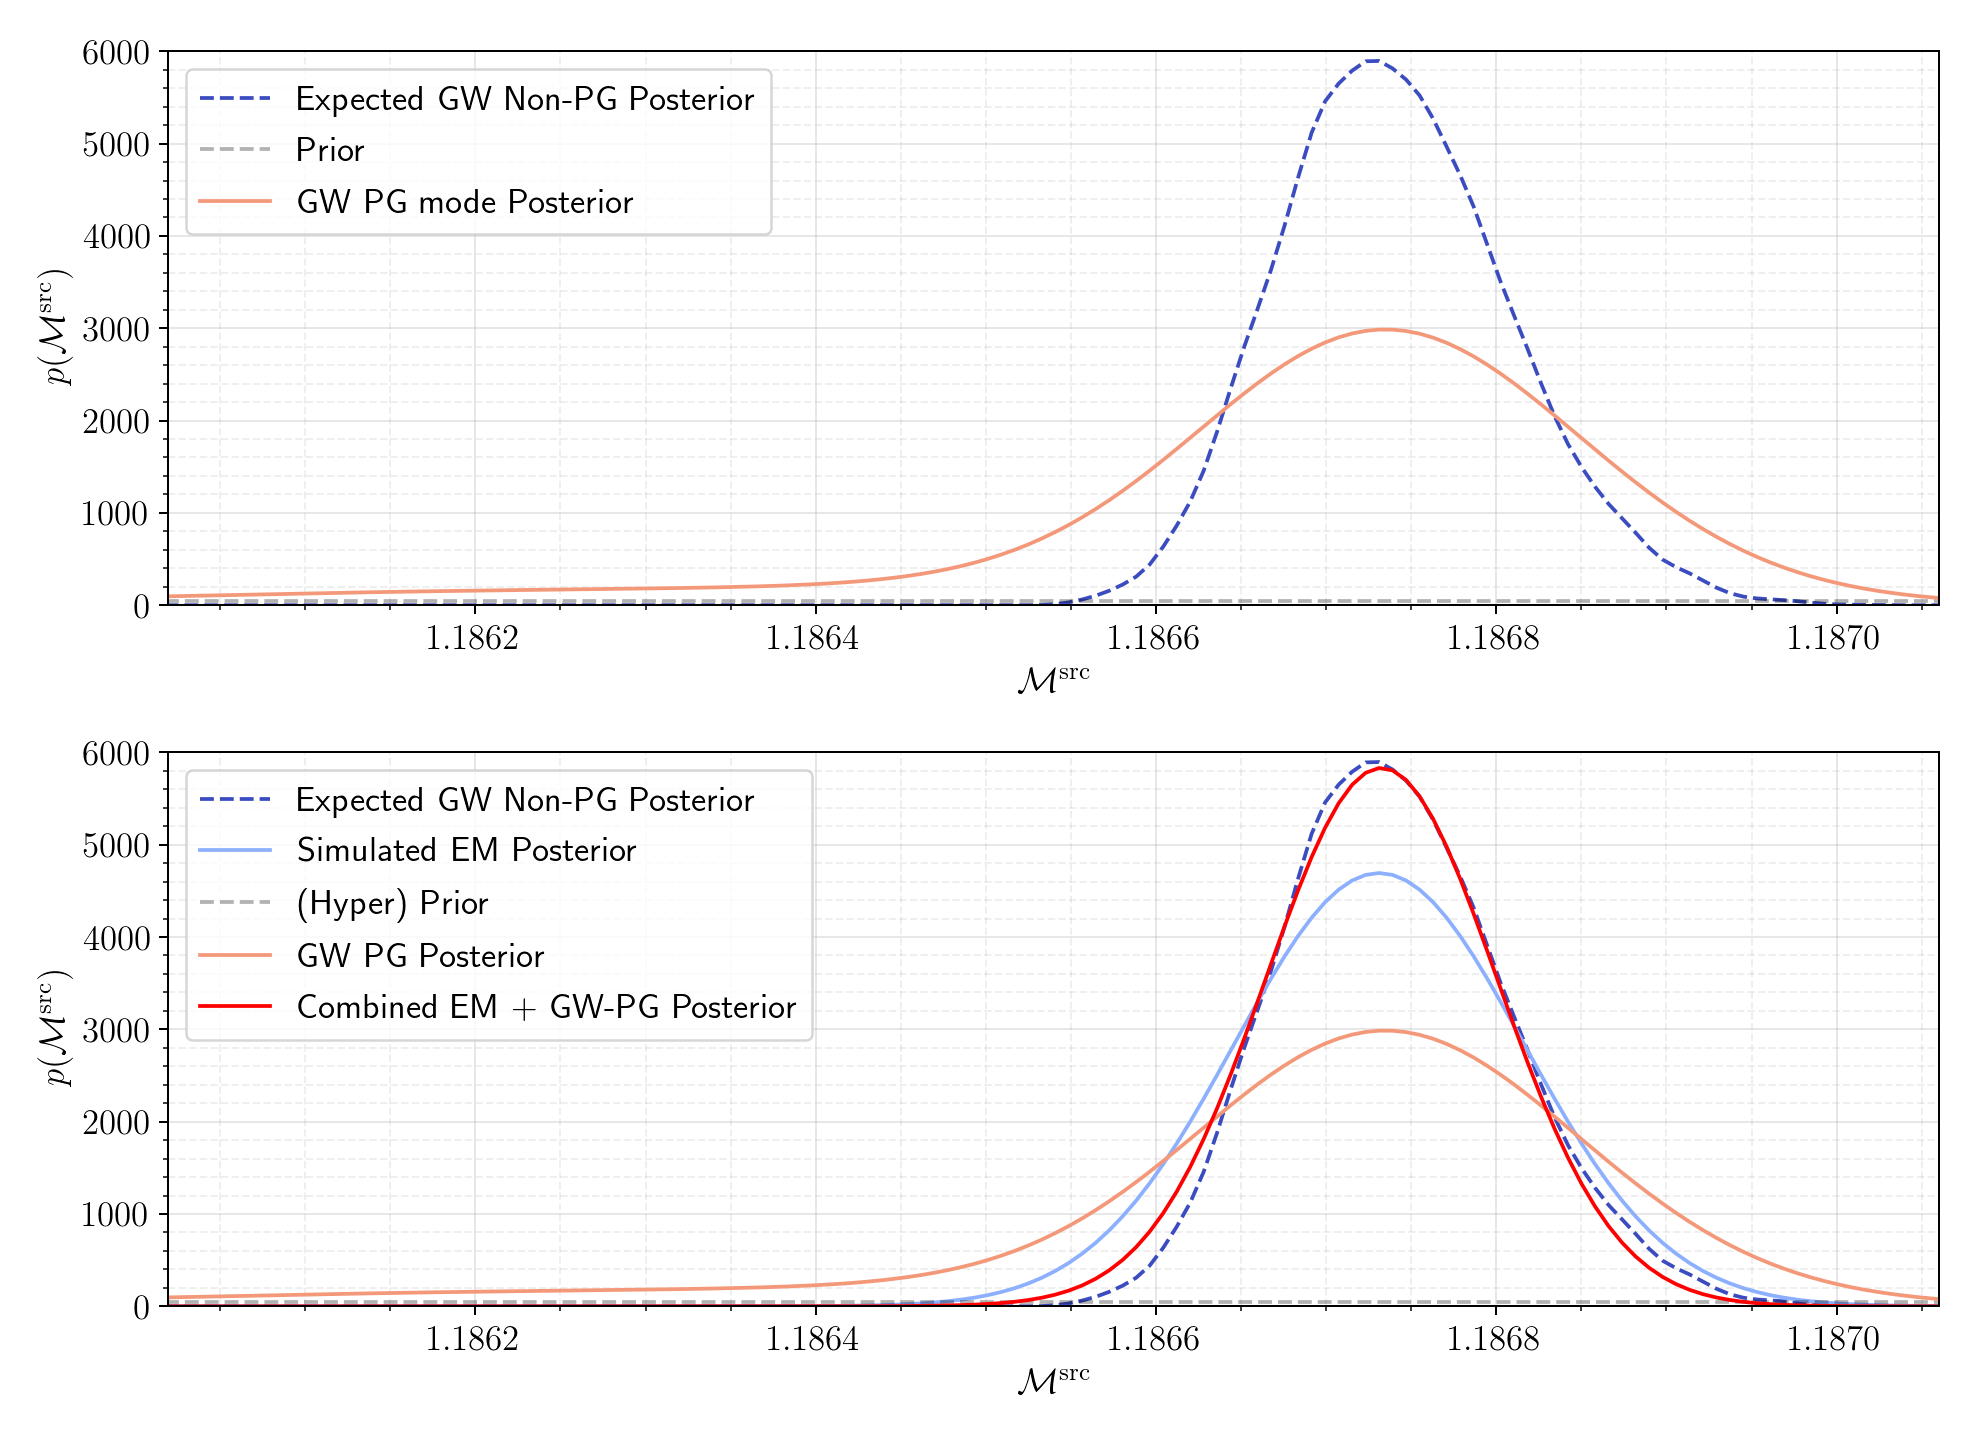
\includegraphics[width=0.9\columnwidth]{figs/chapter6/em_posterior_fix.png}
\caption{(\textit{Top}) The prior distribution on the chirp mass for two gravitational wave astrophysical hypotheses. The first hypothesis is the uniform mass and constrained equation of state constraint model from~\cite{de2018tidal}, while the second model is the $p$-$g$ mode instability hypothesis with unconstrained $\delta \phi$. The marginal posterior distributions on the chirp mass are in dashed-blue and solid, light-red, respectively. (\textit{Bottom}) Combining a simulated Gaussian electromagnetic posterior on the chirp mass (light-blue) and a prior on the chirp mass we can combine the posterior distributions from the gravitational wave data with the $p$-$g$ mode instability from the unconstrained $\delta \phi$ model with this electromagnetic posterior to construct a joint posterior distribution (solid, red) that closely matches the inferred chirp mass for GW170817 from~\cite{de2018tidal}. The simulated Gaussian electromagnetic posterior has mean centered at the maximum a posteriori value from~\cite{de2018tidal}, $\mu = 1.186731 \, M_\odot$, and standard deviation, $\sigma = 0.000085 \, M_\odot$.}
\label{fig:em_posterior_analysis}
\end{figure}


\subsection{Strict Constraints on the $p$-$g$ mode instability}
Given the observed parameter degeneracies, We now investigate regions of the parameter space where nonlinear tidal effects are not degenerate with standard waveforms by thresholding the prior distribution of $p$-$g$ waveforms on their fitting factor with standard waveforms. We combine the results of our analysis on the uniform mass, $\delta \phi$ constrained, narrow $f_0$ prior distribution model to obtain $22,600$ independent samples. We then examine the fitting factor of every independent sample, from every temperature, with a non-spinning, mass-only template bank of TaylorF2 waveforms with comparable masses to GW170817. For simplicity, we only keep the mass parameters and $p$-$g$ mode parameters in the overlap calculations, since the correlation between nonlinear tidal dynamics is most apparent in the measured chirp mass. When we examine the fitting factor between nonlinear tidal waveforms and this template bank we observe that there is a very high match between standard templates and nonlinear tidal waveforms when $n = 4/3$. The nonlinear tidal waveforms that least match this template bank tend to be those parameterized by large amplitude and large gravitational-wave phase shift. We then recompute the Bayes factor when discarding samples from the analysis below a particular fitting factor with the template bank. To ensure a robustness of the point-estimate we use a bootstrap method to estimate the Monte Carlo error for this Bayes factor estimate~\citep{efron1992bootstrap}. The bootstrap estimated Monte Carlo error tends to be much larger than the convergence error for this analysis and so we neglect inclusion of convergence error in the estimate. A statistically significant Bayes factor of $\sim 30 \, (20)$, against nonlinear tides, is found when the waveform has an overlap less than $98.5 \, (98.85)$\% match with the standard waveform, see Fig.~\ref{fig:bayes_ff_plot}. While this metric is insufficient to rule out the $p$-$g$ mode instability, it is a useful metric in understanding why the evidence is nearly identical to the evidence from~\cite{de2018tidal}. We find that portions of the $p$-$g$ mode parameter space that most contribute towards the evidence come from regions of the parameter space that have a high overlap with standard waveforms. This occurs either through $A$ being too small to induce a large change in the phase of the waveform or through an associated parameter degeneracy with the chirp mass caused by large $A$, low $f_0$, and $n \sim 4/3$.

\begin{figure}[th]
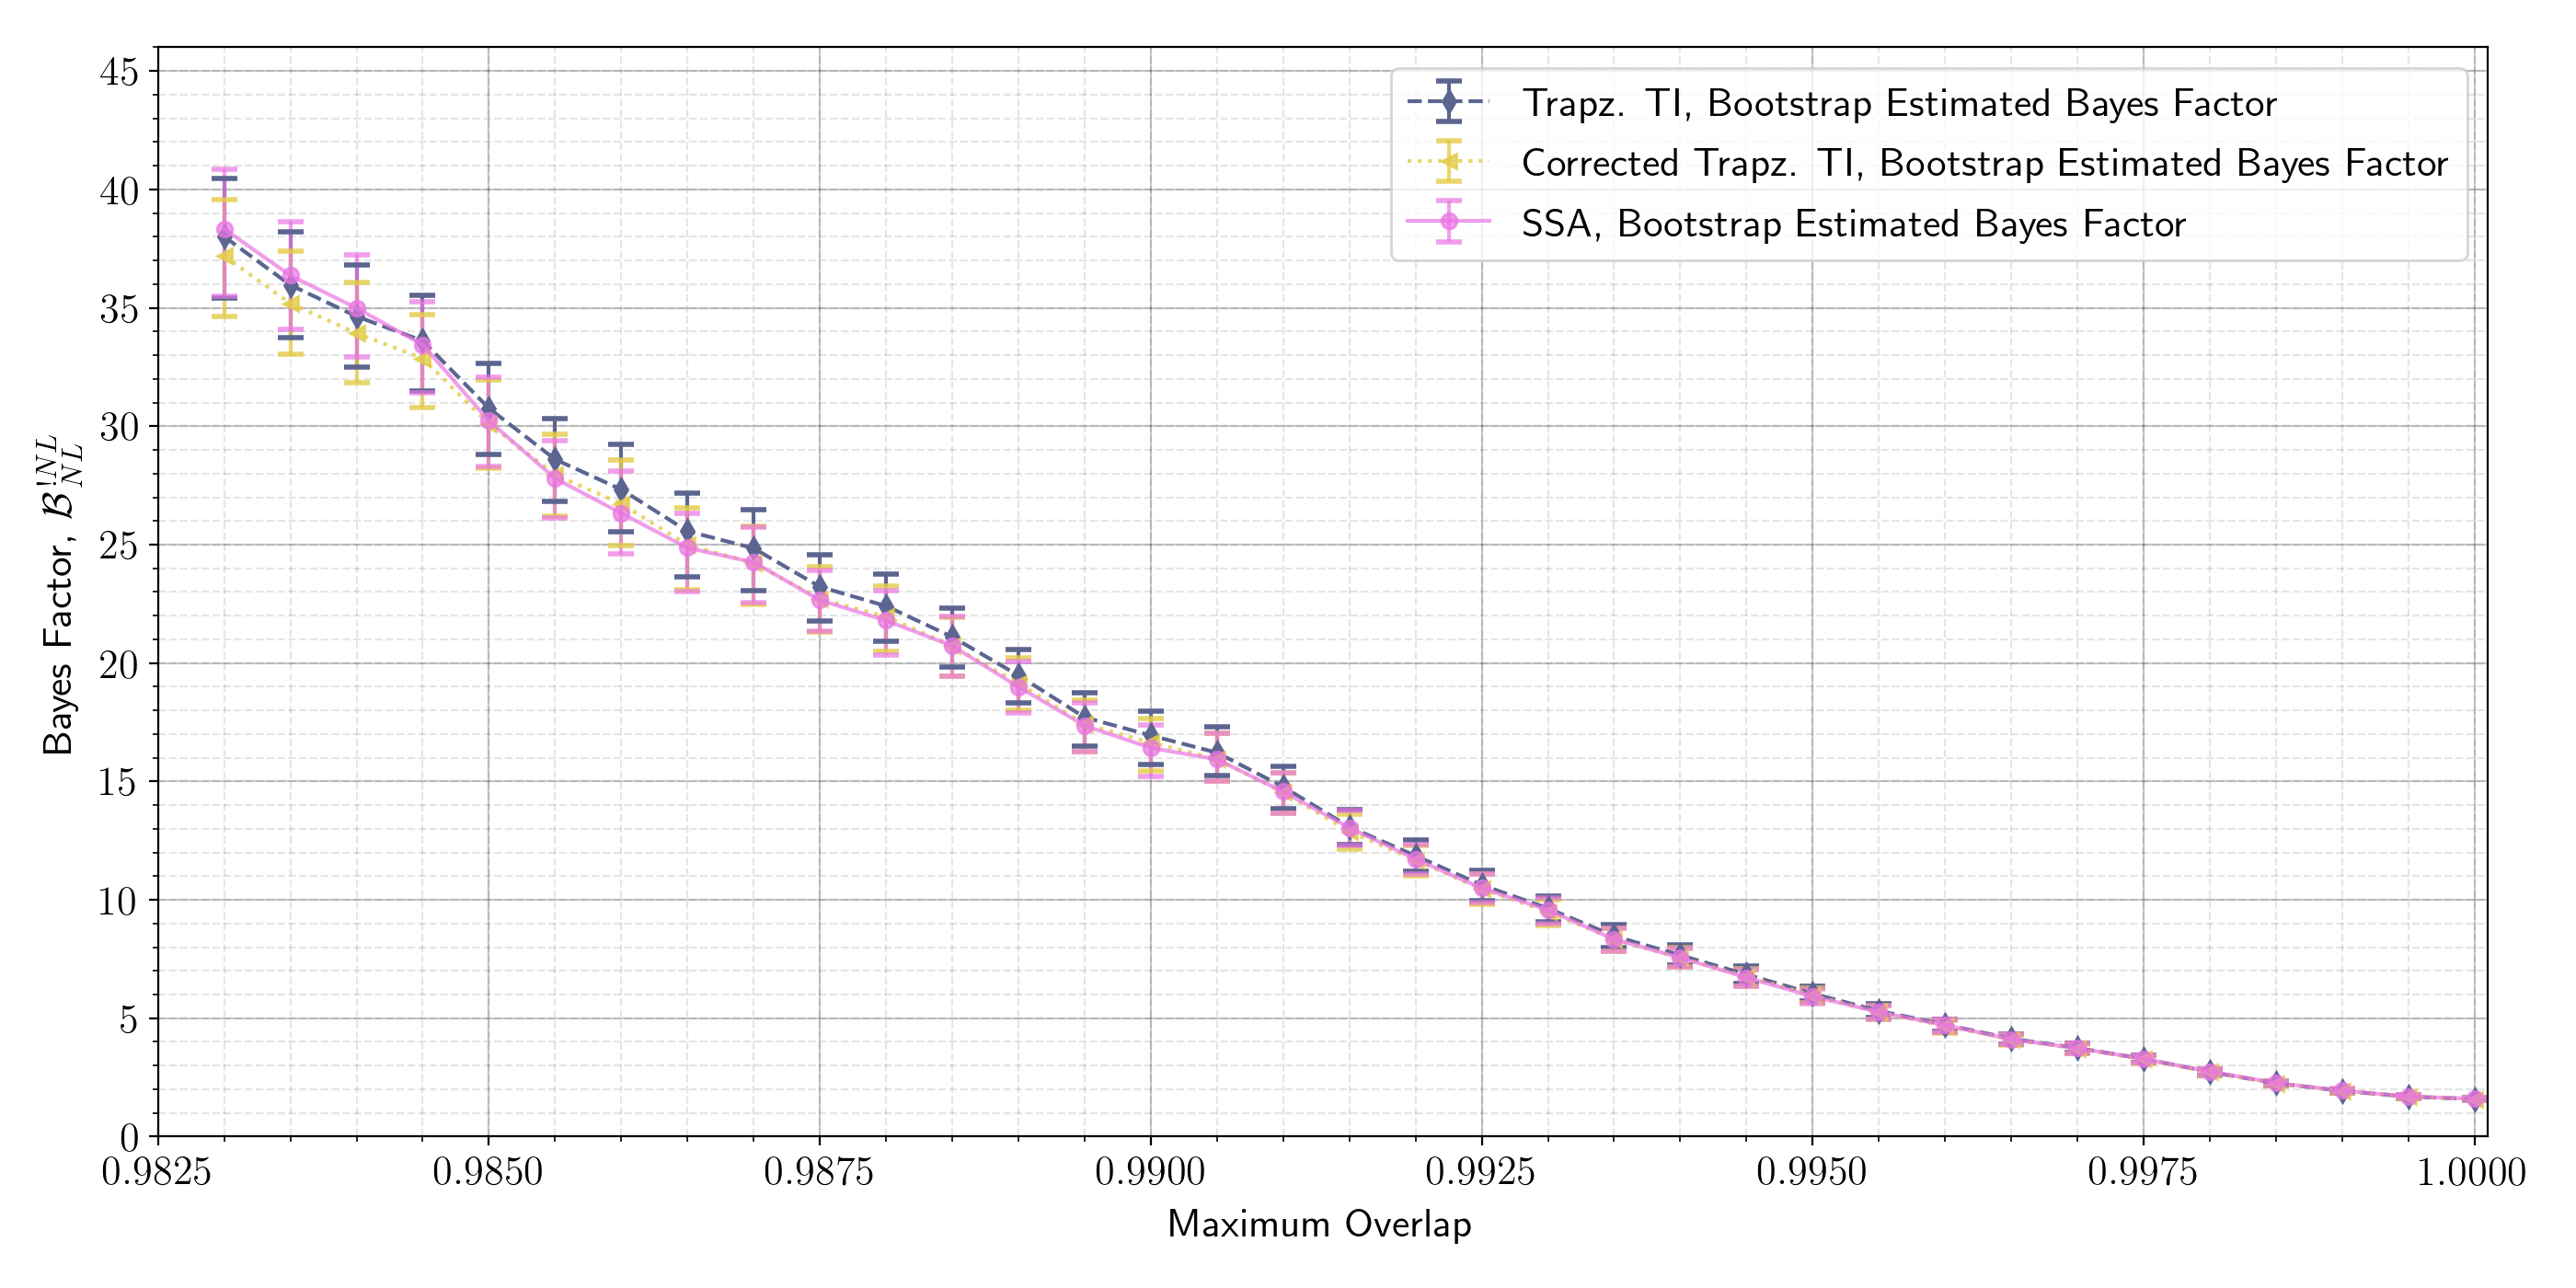
\includegraphics[width=\columnwidth]{figs/chapter6/bootstrap_bayes_ff_cuts_average}\caption{The estimated Bayes factors for nonlinear tidal parameters when the samples are filtered by the fitting factor to a non-spinning, mass-only template bank of TaylorF2 waveforms. The convention in Bayes factor is switched from the main body of the text to represent the Bayes factor for the ratio of evidence for no nonlinear tides, $p\left(\mathbf{d}\,|\, \mathrm{H}_\mathrm{TaylorF2}\right)$, to the evidence for nonlinear tides, $p\left(\mathbf{d}\,|\,\mathrm{H}_\mathrm{TaylorF2+NL}\right)$. This is abbreviated as $\mathcal{B}^{\,\mathrm{!NL}}_{\,\mathrm{NL}}$. The three methods for estimating the Bayes factor are the thermodynamic integration method from trapezoid rule integration (dark grey, dashed line), the thermodynamic integration method from the higher order trapezoid rule (yellow, small-dashed line), and the steppingstone algorithm (dark pink, solid line). A bootstrap method is used to estimate approximate errors on the Bayes Factors. Error bars represent $5^{\mathrm{th}}$ and $95^{\mathrm{th}}$ percentiles. The sampling error becomes large at a fitting factor $\lesssim 99$\%.
}
\label{fig:bayes_ff_plot}
\end{figure}

Finally, we examine the leading order estimated energy dissipated through nonlinear tides for the case of a uniform prior on the mass, with $15 \leq f_0 \leq 100$~Hz, with a $\delta \phi$ $>$ $0.1$ radian constraint. In our analysis, the $95^{\mathrm{th}}$ percentile of the estimated energy dissipated through nonlinear tides from our prior distribution is approximately $2.6 \times 10^{51}$~ergs at the terminating frequency of the TaylorF2 waveform, $f_\mathrm{ISCO}$. The estimated energy radiated by gravitational waves by neutron stars of the estimated mass range of GW170817 is greater than $\sim 10^{53}$~ergs. Our analysis finds the energy dissipated through nonlinear tides at the $95\%$ posterior credible percentile is $3 \times 10^{50}$~ergs. We find our $95\%$ posterior credible percentile to be less than the $90\%$ confidence interval constraint of $\lesssim 2.7 \times 10^{51}$~ergs in~\cite{abbott2019constraining}. Samples from our posterior distribution that have dissipation energies greater than the $90$\% credible interval tend to come from two modes in the parameter space. The first mode is from parts of the parameter space with large $A$, for $n \sim 4/3$, low $f_0$, and $\delta \phi \sim 100$~rad. The second mode is from parts of the parameter space with $A \gtrsim 10^{-8}$, for $1.6 \lesssim n < 3.0$, and $\delta \phi \sim 1-10$~rad. The high end of the nonlinear tidal energy constraints are thus dominated by waveforms that are degenerate with the standard signal.

\section{Discussion}
We have used the observation of GW170817 and the model of~\cite{Essick:2016tkn} to look for evidence of nonlinear tides from $p$-$g$ mode coupling during the inspiral~\citep{Weinberg:2013pbi,Weinberg:2015pxa,Zhou:2018tvc}. Over the broad prior space, we find a Bayes factor of unity which gives an inconclusive result on whether nonlinear tides are favored or disfavored in GW170817, consistent with \cite{abbott2019constraining}. This Bayes factor can be interpreted as stating that there is insufficient evidence to change our prior beliefs about the credibility of the $p$-$g$ mode hypothesis after the observation of GW170817. A closer examination of the posterior distribution lead us to conclude that nonlinear tides are consistent with the signal GW170817 because they either cause very small phase shifts to the waveform, or the nonlinear tides must enter the waveform in a way that is degenerate with the other intrinsic parameters of GW170817. Regions of the nonlinear tide parameter space that have a fitting factor of less than 99\% (98.5\%) are  disfavored by a Bayes factor of 15 (25). we find that waveforms from a $p$-$g$ mode instability with overlap $>98.5$ \%, tend to either induce a very small phase shifts to the waveform or are degenerate with other intrinsic parameters of GW170817. This leads us to conclude that modeling GW170817 with nonlinear tidal parameters may not offer advantages over using a simpler model. We conclude that the consistency of the GW170817 signal with the model of \cite{Essick:2016tkn} is due to parameter degeneracy and that regions where nonlinear tides produce a measurable effect are strongly disfavored.

In principle, one could improve our analysis by separately parameterizing the amplitude, turn-on frequency, and frequency evolution for each star as in~\cite{abbott2019constraining}. However, we find our results to be broadly consistent with~\cite{abbott2019constraining}, and so we do not expect these to affect the main conclusion of our paper. Further improvements on the  parametric model of $p$-$g$ mode instability could include a higher order post-Newtonian expansion of the instability, or further understanding of the instability's interaction with neutron star magnetic fields~\citep{Weinberg:2015pxa}. Nonlinear tides are poorly understood and the contribution from other stellar oscillation modes may yet contribute to a more accurate picture of the interior dynamics of neutron stars~\citep{Andersson:2017iav}. Current models of the gravitational-wave phase shift caused by nonlinear tides from the $p$-$g$ mode instability  suffer from parameter degeneracies with the other intrinsic parameters of a neutron star binary. A measurement of the binary's chirp mass that is independent of gravitational-wave observations would break this degeneracy. However, for a system like GW170817, this would require measurement of the binary's chirp mass to a precision greater than $\sim 0.02 \%$ using an electromagnetic counterpart, which is implausible. Absent improved theoretical understanding of  nonlinear tides from $p$-$g$ mode coupling that can excludes degenerate regions of the parameter space \emph{a priori}, we do not expect this situation to improve with future detections.

We now explore whether it will ever be possible to accumulate sufficient evidence to rule-in, or rule-out the presence of nonlinear tides due to a $p$-$g$ mode instability. We will have to make many assumptions in this section regarding the properties of the model, the events that we see, and the rate of mergers for binary neutron stars.

Our goal is to take advantage of the fact that Bayes factors for hypotheses are multiplicative across statistically independent events. That is to say, that with more binary neutron star events we can accumulate evidence for or against $p$-$g$ mode instability through continuous testing of these hypotheses on the individual events. The Bayes factors for $N$ events can be combined into one Bayes factor via following expression:
\begin{equation}\label{eqn:cumulative_bayes_factor}
    \mathcal{B}(\mathbf{d_1}, \mathbf{d_2}, \ldots,  \mathbf{d_{N-1}}, \mathbf{d_{N}} \, | \, \mathrm{H}_{\mathrm{NL}}, \mathrm{H}_{\mathrm{!NL}}) = \prod_{i=1}^N \mathcal{B}(\mathbf{d_i} \, | \, \mathrm{H}_{\mathrm{NL}}, \mathrm{H}_{\mathrm{!NL}}).
\end{equation}
Here the hypotheses for $p$-$g$ mode instability is denoted as $\mathrm{H}_{\mathrm{NL}}$, while the null hypothesis is denoted $\mathrm{H}_{\mathrm{!NL}}$. Note that inference with Bayes factors is equivalent to a Frequentist inference based on the likelihood rather than inference on a posterior probability. We multiply the Bayes factor by a $50 - 50$ prior odds ratio, $\left(\frac{\pi(\mathrm{H}_{\mathrm{NL}})}{\pi(\mathrm{H}_{\mathrm{!NL}})}\right)$, effectively stating no preference for either hypothesis, to convert the Bayes factor to a posterior odds ratio $\mathcal{O}$. Doing so permits us to consider the posterior odds ratio as equivalent to the Bayes factor:
\begin{equation}\label{eqn:posterior_odds_ratio}
    \mathcal{O}(\mathrm{H}_{\mathrm{NL}}, \mathrm{H}_{\mathrm{!NL}} \, | \, \mathbf{d_1}, \mathbf{d_2}, \ldots,  \mathbf{d_{N-1}}, \mathbf{d_{N}}) = \frac{\pi(\mathrm{H}_{\mathrm{NL}})}{\pi(\mathrm{H}_{\mathrm{!NL}})} \times \mathcal{B}(\mathbf{d_1}, \mathbf{d_2}, \ldots,  \mathbf{d_{N-1}}, \mathbf{d_{N}}\, | \, \mathrm{H}_{\mathrm{NL}}, \mathrm{H}_{\mathrm{!NL}}).
\end{equation}
Here $\mathcal{O}(\mathrm{H}_{\mathrm{NL}}, \mathrm{H}_{\mathrm{!NL}} \, | \, \mathbf{d_1}, \mathbf{d_2}, \ldots,  \mathbf{d_{N-1}}, \mathbf{d_{N}})$ is the posterior odds ratio, and thus setting  $\frac{\pi(\mathrm{H}_{\mathrm{NL}})}{\pi(\mathrm{H}_{\mathrm{!NL}})}$ equal to unity makes the posterior odds ratio equivalent to the Bayes factor. We will use the Bayes factor instead of the odds ratio for the duration of this section, with the understanding that they are equivalent in this scenario.

It is instructive to examine the behavior of the cumulative logarithm of the Bayes factor for the incredible case that the next several binary neutron stars are identical in signal-to-noise ratio and intrinsic properties as GW170817. Here we consider two estimators for the Bayes factor, the thermodynamic integration method which we found to have a log Bayes factor of $\mu \sim -0.38$, and at worst $\sigma \sim 0.1$, and the logspline estimator with the Savage Dickey density ratio which we found to have a log Bayes factor of $\mu \sim -0.46, \sigma \sim 0.06$. We note that the logspline estimate is not a log-normal distribution, but it this estimate is close enough to the estimates from our analysis for demonstrative purposes. The analysis of~\cite{abbott2019constraining} found a log Bayes factor of $0.03^{+0.70}_{-0.58}$ at $90 \%$ confidence using the Savage-Dickey density ratio. We model this as a Gaussian distribution in the logarithm Bayes factor with $\mu = 0.03, \sigma = 0.4$ so as to have a similar $90\%$ interval width. While for GW170817 these Bayes factor estimates are compatible, if we measure a new GW170817-like binary neutron star and measure the same Bayes factor for this new event, the cumulative Bayes factor and the uncertainty surrounding this cumulative Bayes factor propagates multiplicatively and quickly begin to exclude each other as more events are aggregated.

To illustrate this consider the case that our MCMC methods estimate the logarithm of Bayes factors for some fixed choice of prior distribution and for cumulative gravitational wave events. Consider the case that the estimator of the logarithm of the Bayes factor is a normal distribution with mean (point-estimate) $\mu$ and a standard deviation (uncertainty) $\sigma_i$:
\begin{equation}
    \widehat{\mathrm{ln} \, \mathcal{B}^{\mathrm{NL}}_{\mathrm{!NL}}}(\mathbf{d_i}) = \mathcal{N}(\mu_i, \sigma_i).
\end{equation}
Thus, the cumulative Bayes factor for many neutron star events becomes:
\begin{equation}
    \begin{array}{ll}
    \widehat{\mathrm{ln} \, \mathcal{B}^{\mathrm{NL}}_{\mathrm{!NL}}}(\mathbf{d_1}, \mathbf{d_2}, ..., \mathbf{d_N}) &\quad = \sum \limits_{i=1}^{N} \widehat{\mathrm{ln} \, \mathcal{B}^{\mathrm{NL}}_{\mathrm{!NL}}}(\mathbf{d_i}) \\ \\
    &\quad = \mathcal{N}\left(\mu = \sum \limits_{i=1}^{N} \mu_i, \, \, \sigma = \sqrt{\sum \limits_{i=1}^{N} \sigma_i^2}\right).
    \end{array}
\end{equation}
We note that if the Bayes factor point-estimate term $\mu_i$ is monotonic across events, and the uncertainty estimate from our MCMC methods $\sigma_i$ is usually consistent, then the estimator $\widehat{\mathrm{ln} \, \mathcal{B}^{\mathrm{NL}}_{\mathrm{!NL}}}(\mathbf{d_1}, ..., \mathbf{d_N})$ will tend towards a log Bayes factor that is statistically significant, for which a decision on whether nonlinear tidal effects from a $p$-$g$ mode instability is present / measurable in neutron stars.  For repetitions of the same event we see that the mean of this Gaussian distribution for the cumulative log Bayes factor grows linearly with $mu_i$, and the uncertainty grows as $\sqrt{N} \sigma_i$. However, if noise elements in the MCMC or from the data itself dilute the ability for our MCMC estimator to find a $\mu \neq 0$ or a monotonic measurement of $\mu$ then the logarithm of the Bayes factor will become overly diluted by a growing uncertainty $\sigma$.  As seen in Fig.~\ref{fig:sim_many_gw170817_divergent_bayes}, after five events, the cumulative Bayes factor estimations diverge significantly. They may be caused by different methodologies in Bayes factor estimation, by waveform systematics, by power-spectral density estimation differences, by different segments of GPS-analysis times used, the low-frequency cutoff used, or by many other possible variables that are not accounted for in this comparison. As MCMC methods for estimating Bayes factor improve this error in cumulative Bayes factor estimation should also improve.

\begin{figure}[th]
\centering
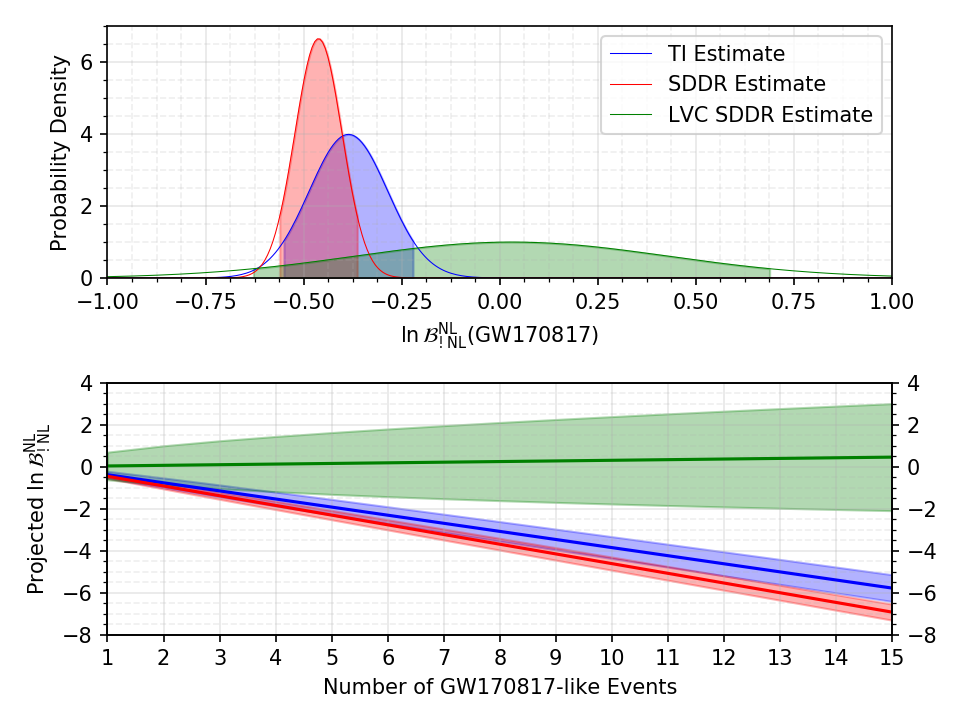
\includegraphics[width=0.9\columnwidth]{figs/chapter6/sim_many_gw170817_evidence_error_prop.png}
\caption{(\textit{Top}) A comparison of Gaussian approximations of the logarithm of the Bayes factor using different estimators or waveform systematics. Note that the LVC estimate here is a rough Gaussian approximation based on the reported bounds in~\cite{abbott2019constraining}. The $90 \%$ confidence regions are shaded in. Positive log Bayes factors are indicative of support for the $p$-$g$ mode hypothesis, while negative log Bayes factors are indicative of support for the null hypothesis. (\textit{Bottom}) For repeated GW170817-like binary neutron star mergers the cumulative logarithm of the Bayes factor for the $p$-$g$ mode hypothesis vs the null hypothesis begin to diverge in estimation. The solid lines represent the cumulative median estimates, while the shaded regions represent the cumulative $90 \%$ confidence intervals. Waveform systematics or uncontrolled variables in the Bayes factor estimation methods may be the main driver of this divergence and future meta-analyses will have to control for these sorts of uncertainty.}
\label{fig:sim_many_gw170817_divergent_bayes}
\end{figure}

A more realistic approach is to consider that the distribution of signal-to-noise ratio for binary neutron star events will not all be repeats of GW170817 but rather will follow some other distribution. To do so explore this we need to model the expected signal-to-noise-ratio, $\rho$, of events that we expect to see with gravitational wave observatories. Fortunately, this work has already been done in~\cite{schutz2011networks, chen2014loudest}. We can expect that for a network of interferometers with a signal to noise ratio detection threshold of $\rho_{\mathrm{threshold}}$ that our distribution will follow the rule:
\begin{equation}\label{eqn:universal_snr}
    p(\rho) = 3 \, \frac{\rho_{\mathrm{threshold}}^3}{\rho^4}.
\end{equation}
This expression is a normalized probability distribution function in so far as we only permit $\rho > \rho_{\mathrm{threshold}}$ and let $\rho$ go to positive infinity. Given this probability distribution we can expect our average $\rho$ to be equal to $\frac{3}{2} \rho_{\mathrm{threshold}}$. If we assume a very conservative $\rho_{\mathrm{threshold}} = 11$, then the probability of attaining gravitational wave neutron star mergers as loud as or louder than GW170817 ($\rho \approx 34$) is slightly higher than $3~\%$. At a signal-to-noise ratio of $\sim 34$ we have found that the $p$-$g$ mode instability hypothesis has a Bayes factor of approximately $1$, and we expect that $97 \%$ of neutron star detections will be quieter than GW170817 for which the Bayes factor will in all likelihood be unity as well due to parameter degeneracies. Thus we see that in the long-term we may have to wait for hundreds of binary neutron star mergers to be able to make a decision on the validity of the $p$-$g$ mode instability hypothesis, for-or-against. Biases and difficulties in the MCMC method for hypothesis testing, the noise in the detector, and waveform systematics in all likelihood will make this endeavor all the more difficult.

And so to the question, ``Will there ever be a time when we can rule out $p$-$g$ mode instability?", depends on a number of factors. Firstly, what do we mean when we say the $p$-$g$ mode instability, e.g., which prior distribution choices, which waveform model, what post-Newtonian order of the waveform model, with which MCMC method, and under applications of the matched-filtering method? We have in this work ruled out some $p$-$g$ mode instability hypotheses through the observation of GW170817. In addition, the marginal posterior densities from~\cite{abbott2019constraining} similarly tell us that some $p$-$g$ mode parameters are not favored by the data. With current observations it is not possible to rule out the theory entirely, but future events may shed more light on the possibility of nonlinear tides in neutron stars. Perhaps a more important result of this analysis is the ambiguity and difficulties inherent in Bayesian gravitational wave astrophysical analysis. We hope that our exploration and explanation of the problem prompts greater thoughtfulness with respect to statistical analysis and experimental design.

\newpage
\begin{table}[ht]
\begin{adjustbox}{angle=90}
\begin{tabularx}{1.0\textwidth}{l c c c c c c}
\hline\hline
 Hypothesis Tested  & $\mathcal{B}^{\mathrm{NL}}_{\mathrm{!NL}}(A)$  & $\mathcal{B}^{\mathrm{NL}}_{\mathrm{!NL}}(B)$ & $\mathcal{B}^{\mathrm{NL}}_{\mathrm{!NL}}(C)$ & $\mathcal{B}^{\mathrm{NL}}_{\mathrm{!NL}}(D)$ & $\mathcal{B}^{\mathrm{NL}}_{\mathrm{!NL}}(E)$ & $\mathcal{B}^{\mathrm{NL}}_{\mathrm{!NL}}(F)$\\
\hline\hline
$H_1$ (Uniform Mass, $A$, $n$, $f_0$ $\in$ (15, 100) $Hz$), $\delta \phi > 0.1$ &
$0.63^{+0.08}_{-0.07}$ & $0.63^{+0.08}_{-0.07}$ & $0.64^{+0.07}_{-0.06}$ & $0.64^{+0.05}_{-0.05}$ & $0.63^{+0.06}_{-0.06}$ & $0.63^{+0.06}_{-0.06}$ \\ 
\hline
$H_2$ (Gaussian Mass, $A$, $n$, $f_0$ $\in$ (15, 100) $Hz$), $\delta \phi > 0.1$ &
$0.71^{+0.08}_{-0.07}$ & $0.71^{+0.08}_{-0.07}$ & $0.70^{+0.06}_{-0.06}$ & $0.70^{+0.04}_{-0.04}$ & $0.71^{+0.06}_{-0.06}$ & $0.73^{+0.07}_{-0.07}$ \\ 
\hline
$H_3$ (Uniform Mass, $A$, $n$, $f_0$ $\in$ (15, 800) $Hz$), $\delta \phi > 0.1$ &
$0.64^{+0.09}_{-0.08}$ & $0.64^{+0.09}_{-0.08}$ & $0.64^{+0.08}_{-0.07}$ & $0.64^{+0.06}_{-0.06}$ & $0.64^{+0.06}_{-0.06}$ & $0.63^{+0.09}_{-0.07}$ \\ 
\hline
$H_4$ (Gaussian Mass, $A$, $n$, $f_0$ $\in$ (15, 800) $Hz$), $\delta \phi > 0.1$ &
$0.76^{+0.08}_{-0.07}$ & $0.76^{+0.08}_{-0.07}$ & $0.75^{+0.06}_{-0.06}$ & $0.75^{+0.04}_{-0.04}$ & $0.75^{+0.05}_{-0.05}$ & $0.76^{+0.07}_{-0.06}$ \\ 
\hline
$H_5$ (Uniform Mass, $A$, $n$, $f_0$ $\in$ (10, 100) $Hz$) &
$0.68^{+0.12}_{-0.11}$ & $0.68^{+0.13}_{-0.11}$ & $0.69^{+0.11}_{-0.1}$ & $0.69^{+0.1}_{-0.09}$ & $0.67^{+0.1}_{-0.08}$ & $0.65^{+0.13}_{-0.11}$ \\
\hline\hline
\end{tabularx}
\end{adjustbox}
\caption{The various Bayes factors under different multi-tempered integration methods. The column marked with $\mathcal{B}^{\mathrm{NL}}_{\mathrm{!NL}}(A)$ is the Bayes factor under the thermodynamic integration method using the trapezoid quadrature rule. The $(B)$ column is the Bayes factor from the thermodynamic integration method using the higher-order trapezoid quadrature rule. The $(C)$ column is the Bayes factor from the thermodynamic integration method using Simpson's quadrature rule. The $(D)$ column is the Bayes factor for the thermodynamic integration method using Simpson's higher-order quadrature rule. The $(E)$ column is the Bayes factor for the thermodynamic integration method using a cubic polynomial quadrature rule. And $(F)$ is the Bayes factor from the steppingstone method. The $50^{\mathrm{th}}$ percentile with the $5^{\mathrm{th}}$ and $95^{\mathrm{th}}$ percentiles in the plus and minus superscripts and subscripts, respectively, are shown above.}\label{table:Bayes}
\end{table}

%$0.631831831832^{+0.0774774774775}_{-0.0684684684685}$ & $0.631831831832^{+0.0774774774775}_{-0.0690690690691}$ & $0.637237237237^{+0.0678678678679}_{-0.0612612612613}$ & $0.637237237237^{+0.0528528528529}_{-0.0486486486486}$ & $0.633633633634^{+0.0600600600601}_{-0.0546546546547}$ & $0.633633633634^{+0.0600600600601}_{-0.0546546546547}$ \\ 

%$0.708708708709^{+0.0786786786787}_{-0.0708708708709}$ & $0.709309309309^{+0.0786786786787}_{-0.0714714714715}$ & $0.702102102102^{+0.0630630630631}_{-0.0582582582583}$ & $0.701501501502^{+0.0432432432432}_{-0.0408408408408}$ & $0.710510510511^{+0.0606606606607}_{-0.0564564564565}$ & $0.726726726727^{+0.0744744744745}_{-0.0678678678679}$ \\ 

%$0.637237237237^{+0.0864864864865}_{-0.0762762762763}$ & $0.637837837838^{+0.0870870870871}_{-0.0768768768769}$ & $0.640840840841^{+0.0756756756757}_{-0.0678678678679}$ & $0.640840840841^{+0.0624624624625}_{-0.0570570570571}$ & $0.64024024024^{+0.0642642642643}_{-0.0588588588589}$ & $0.631831831832^{+0.0846846846847}_{-0.0744744744745}$  \\ 

%$0.756156156156^{+0.0780780780781}_{-0.0714714714715}$ & $0.756756756757^{+0.0786786786787}_{-0.0714714714715}$ & $0.753153153153^{+0.0636636636637}_{-0.0582582582583}$ & $0.753153153153^{+0.0402402402402}_{-0.0378378378378}$ & $0.74954954955^{+0.0516516516517}_{-0.0474474474474}$ & $0.75975975976^{+0.0672672672673}_{-0.0618618618619}$  \\ 

%$0.678678678679^{+0.124924924925}_{-0.105705705706}$ & $0.677477477477^{+0.126726726727}_{-0.106306306306}$ & $0.688888888889^{+0.10990990991}_{-0.0948948948949}$ & $0.688288288288^{+0.0984984984985}_{-0.0858858858859}$ & $0.66966966967^{+0.0954954954955}_{-0.0834834834835}$ & $0.654654654655^{+0.126726726727}_{-0.106306306306}$ \\ 


\newpage
\begin{table}[ht]
\begin{adjustbox}{angle=90}
\begin{tabularx}{1.0\textwidth}{l c c c c}
\hline\hline
 Hypothesis Tested  & $\mathcal{B}^{\mathrm{NL}}_{\mathrm{!NL}}$(FD)  & $\mathcal{B}^{\mathrm{NL}}_{\mathrm{!NL}}$(Scott) & $\mathcal{B}^{\mathrm{NL}}_{\mathrm{!NL}}$(Gaussian KDE) & $\mathcal{B}^{\mathrm{NL}}_{\mathrm{!NL}}$(Logspline)\\
\hline\hline
$H_5$ (Uniform Mass, $A$, $n$, $f_0$ $\in$ (10, 100) $Hz$) &
$0.66^{+0.08}_{-0.07}$ & $0.66^{+0.08}_{-0.07}$ & $0.66^{+0.13}_{-0.1}$ & $0.63^{+0.06}_{-0.05}$ \\
\hline\hline
\end{tabularx}
\end{adjustbox}
\caption{The various Bayes factors from the Savage-Dickey Density Ratio test under different density estimators. The column marked with $\mathcal{B}^{\mathrm{NL}}_{\mathrm{!NL}}$(FD) is the Bayes factor from the Freedman Diaconis histogram binning rule. The $\mathcal{B}^{\mathrm{NL}}_{\mathrm{!NL}}$(Scott) column is the Bayes factor estimate under Scott's histogram binning rule. The $\mathcal{B}^{\mathrm{NL}}_{\mathrm{!NL}}$(Gaussian KDE) column is the Bayes factor estimate when using the Gaussian kernel density estimator with linear boundary bias corrections as found in the GetDist Python package. The column denoted as  $\mathcal{B}^{\mathrm{NL}}_{\mathrm{!NL}}$(Logspline) is the Bayes factor estimate when using the logspline density estimator. The $50^{\mathrm{th}}$ percentile with the $5^{\mathrm{th}}$ and $95^{\mathrm{th}}$ percentiles in the plus and minus superscripts and subscripts, respectively.}\label{table:Bayes_sddr}
\end{table}

\begin{figure}[th]
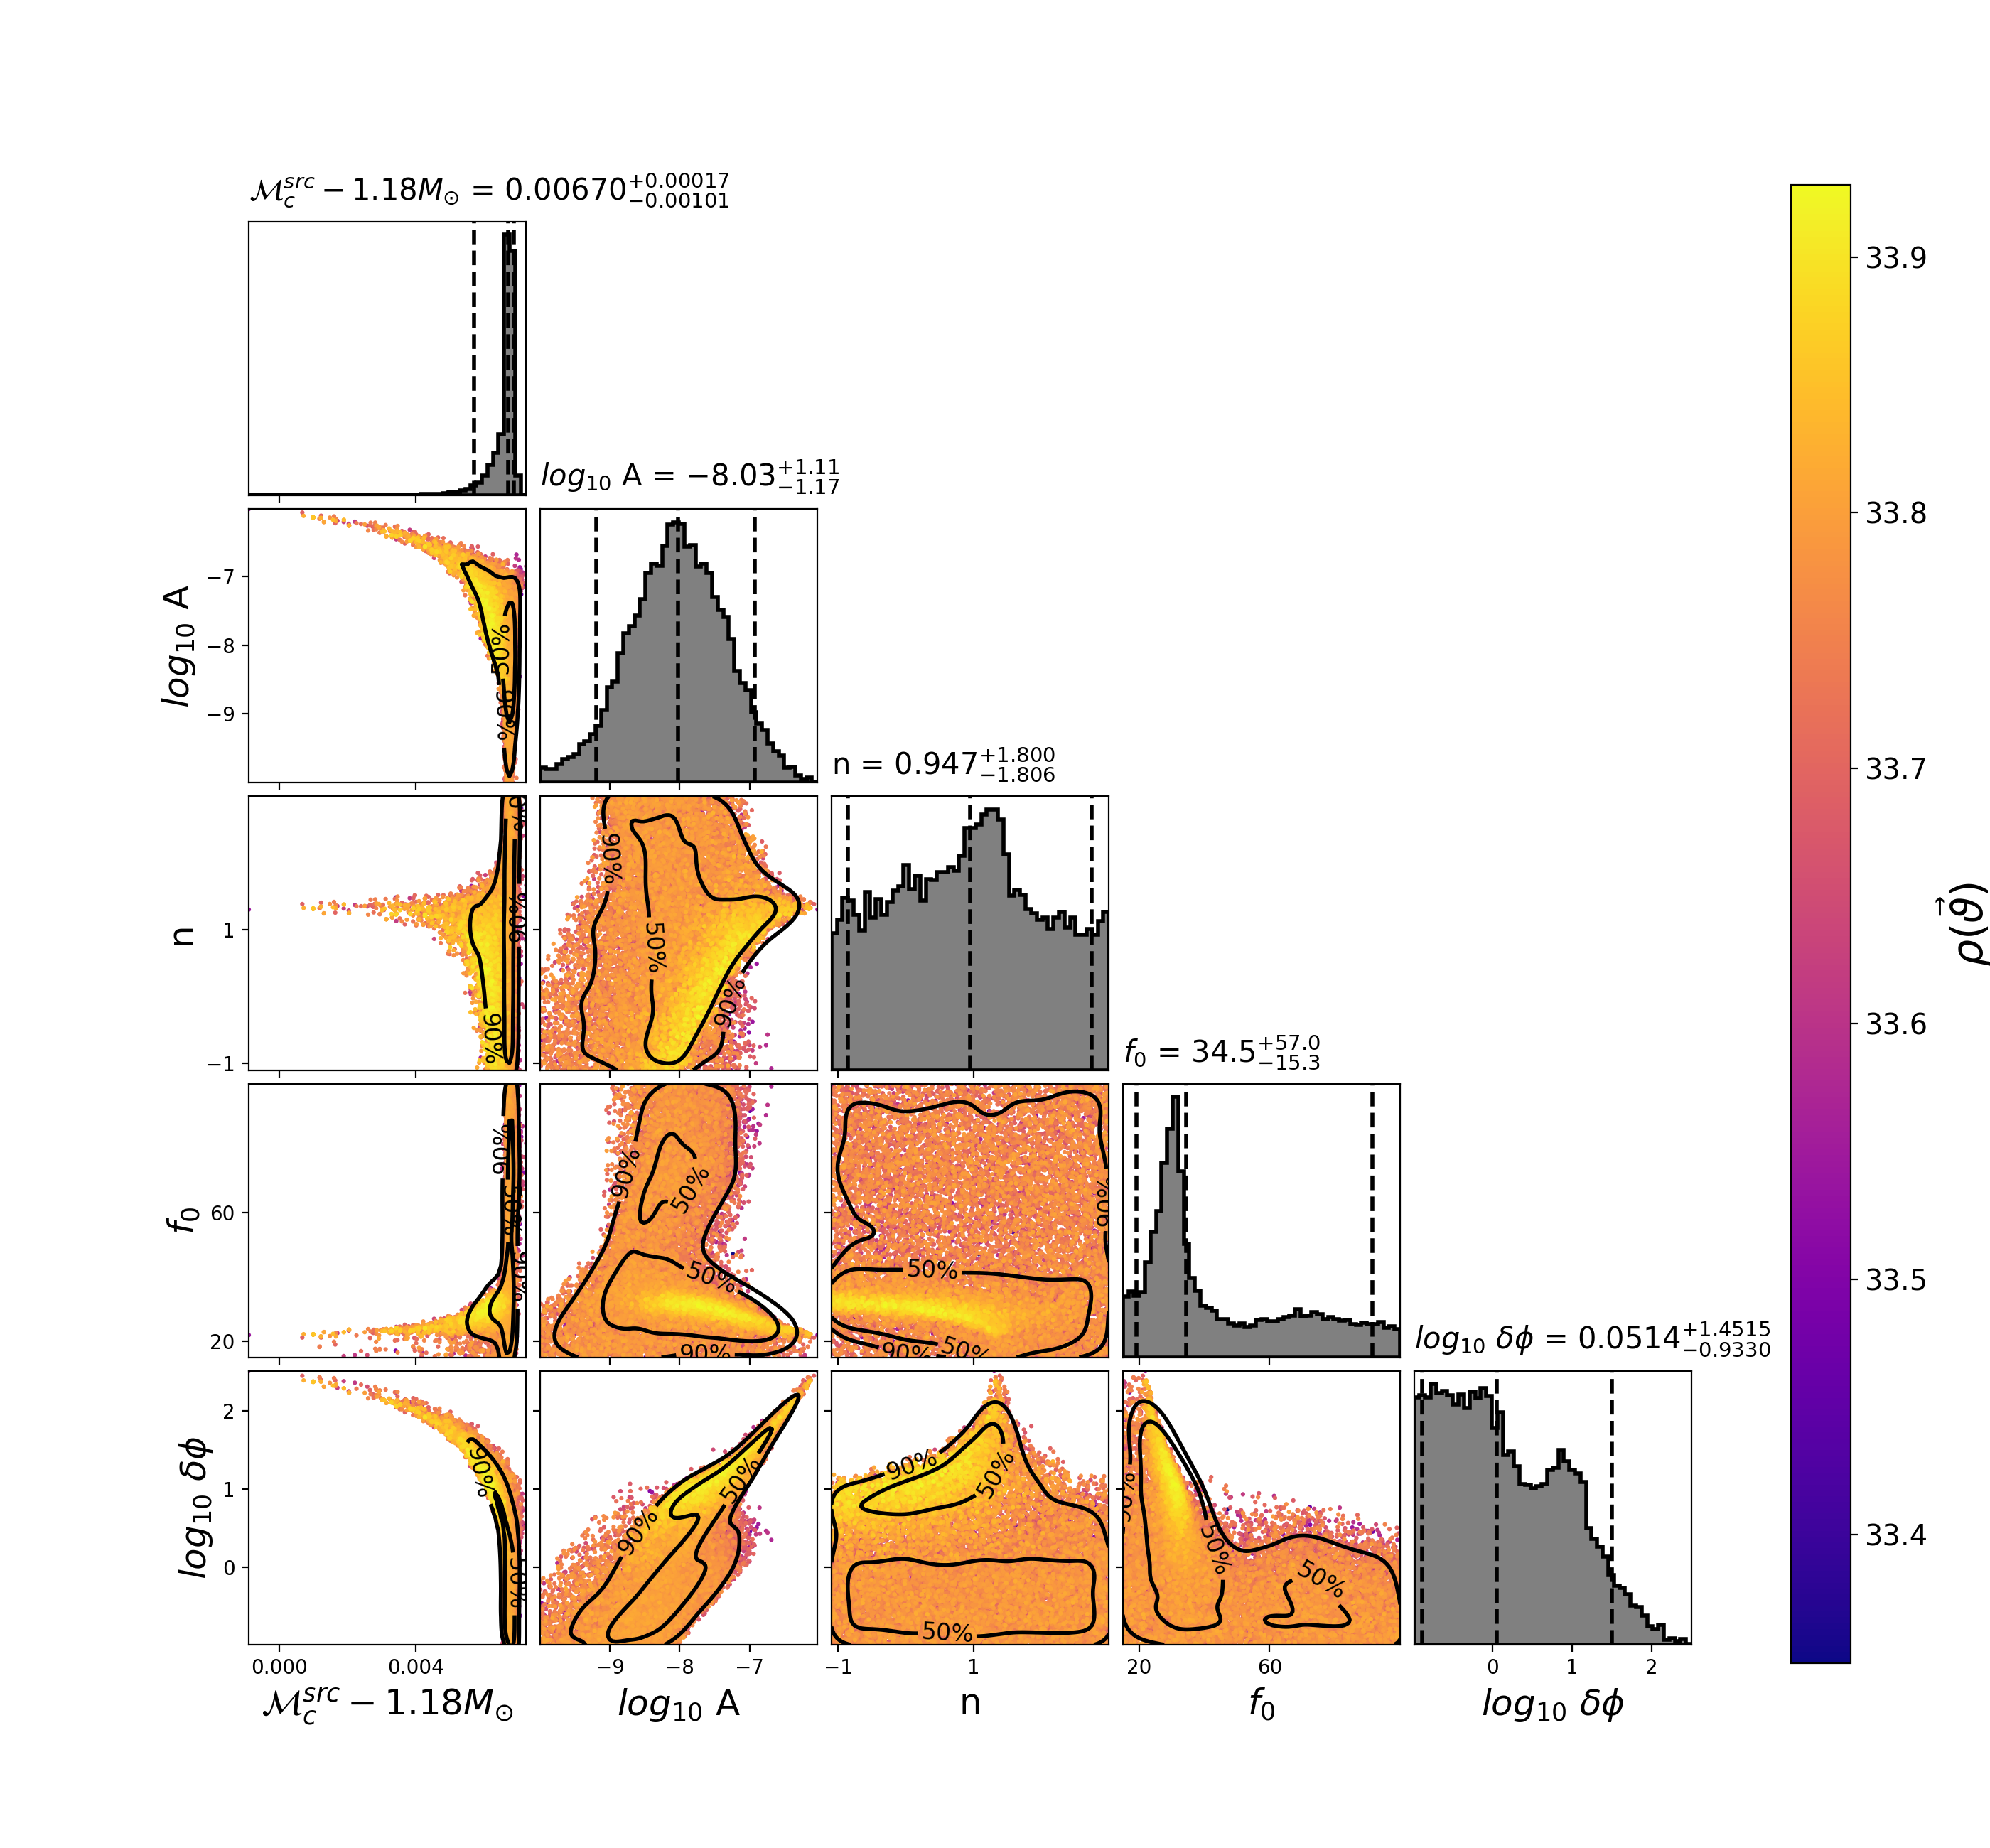
\includegraphics[width=\columnwidth]{figs/chapter6/combined_uni_dphi_cut_combined.png}
\caption{The marginalized posterior distributions for the uniform mass prior and a $f_0$ restricted to the range $15$ and $100$~Hz. The vertical lines on the marginalized histograms display the $5$th, $50$th, and $95$th percentiles of the posteriors. The three-detector network signal-to-noise ratio for each sample is given on the color-bar. The posterior scatter plots show 50\% and 90\% credible interval contours. The posteriors on $n$ is peaked $n \lesssim 4/3$ and for values of $f_0$ close to the lower end of the detector's low frequency sensitivity. In this region of parameters space, the effect of nonlinear tides is degenerate with chirp mass, causing a secondary peak in the chirp mass posterior. It can be seen from the $\delta\phi$--$\mathcal{M}$ plot (lower left) that large phase shifts due to nonlinear tides are due to points in parameter space where a value of chirp mass can be found that compensates for the phase shift of the nonlinear tides. These are the combined posteriors from $9$ runs. It is notable that the the peaks in the $f_0$ posterior, at $f_0 \approx 30$~Hz and $f_0 \approx 70$~Hz seem to be reversed from those in Fig 2. of \citep{abbott2019constraining}. Note that the marginalized posterior for $A$ is diminished for $A < 10^{-8}$ due to the $\delta \phi$ prior constraint.
}
\label{fig:uniform_f0_small}
\end{figure}



\Chapter{Practical Considerations for Bayesian Model Comparison}
\label{ch:bayes_factors}
\section{Bayes factor approaches to Model Selection}
\subsection{Arithmetic Mean Estimator}
The simplest numerical integration estimation of the marginal likelihood makes use of a very large amount of samples drawn from the prior $\pi(\theta)$. For this estimator, Eq. N is approximated as:
\begin{equation}\label{AME}
    \mathcal{Z} \sim \frac{1}{N} \sum_{i=1}^{N} \mathcal{L}_i \left(\theta\right).
\end{equation}
Where N is the number of samples drawn from the prior. We can express Eq. \ref{AME} in the logarithmic form as:
\begin{equation}\label{logAME}
    ln \, \mathcal{Z} \sim  ln \, \mathcal{L}_\mathrm{max} + ln \, 
    \left [ \frac{1}{N} \sum_{i=1}^{N} e^{\left(ln \, \mathcal{L}_i - ln \, \mathcal{L}_\mathrm{max} \right)} \right ].
\end{equation}
While simple to compute, most practical applications have very sharply peaked posterior distributions relative to the prior distribution and so the arithmetic mean estimator can suffer from large variance (). Due to the disparity in the volume of the prior distribution and the posterior distribution, the arithmetic mean estimator can systematically underestimate of the marginal likelihood. In practice, this method requires an extremely large number of samples from the prior (even for low-dimensional models, typically $> 10^9 samples$).

Show average ln Z vs samples, with bootstrap estimated variance of ln Z vs samples. Very large. Not practical.

\subsection{Harmonic Mean Estimator}
The harmonic mean estimator tackles the problem of sharply peaked posterior distribution directly by averaging over the sum of the log-likelihood as drawn from the posterior distribution. Consider the following expression of the reciprocal of the marginal likelihood:
\begin{equation}\label{HMEsub1}
\int \frac{\mathcal{P}(\theta \mid D)}{\mathcal{L}\left(D \mid \theta\right)} d\theta. 
\end{equation}
If one substitutes $\mathcal{P}(\theta \mid D) = (1/\mathcal{Z}) \, \mathcal{L}(D \mid \theta) \, \pi (\theta)$ into Eq. \ref{HMEsub1}, one recovers the following expression:
\begin{equation}\notag
\frac{\int \pi(\theta) d\theta}{\mathcal{Z}} = \int \frac{\mathcal{P}(\theta \mid D)}{\mathcal{L}\left(D \mid \theta\right)} d\theta 
\end{equation}
Now, the prior distribution is always normalized to integrate to $1$ and so the above expression becomes:
\begin{equation}\label{HME}
\frac{1}{\mathcal{Z}} = \int \frac{\mathcal{P}(\theta \mid D)}{\mathcal{L}\left(D \mid \theta\right)} d\theta  = \left \langle \frac{1}{\mathcal{L}(D\mid \theta)} \right \rangle_{\mathcal{P}(\theta \mid D) }
\end{equation}
Thus the inverse of the marginal likelihood can be estimated by the expecation value of the inverse of the likelihood when drawn from the posterior distribution. It is sometimes stated in the statistics literature as, the expectation value of the inverse of the likelihood where the probability measure value is defined by the posterior distribution (). To estimate the marginal likelihood from actual discrete samples drawn from the posterior distribution we can rewrite Eq. \ref{HME} as:
\begin{equation}\label{estim_HME}
    \mathcal{Z} \sim \left(\frac{1}{N} \sum_{i=1}^{N} \frac{1}{\mathcal{L}_i} \right)^{-1}.
\end{equation}
Here $N$ represents the number of samples drawn from the posterior distribution. In the logarithmic form we can express this as:
\begin{equation}\label{estim_logHME}
    ln \, \mathcal{Z} = -ln \, \mathcal{L}_\mathrm{max} - ln \, \left [\frac{1}{N} \sum_{i=1}^{N} e^{-ln \, \mathcal{L}_i -ln \, \mathcal{L}_\mathrm{max}} \right].
\end{equation}
While drawing from the posterior may seem like a more efficient method of estimating the marginal likelihood than drawing from the prior this method is known to sometimes  overestimate the marginal likelihood. Furthermore, this estimator formally has an infinite variance, although the measured variance from samples may not be as large depending on the shape of the posterior distribution. Because of the large variance, the convergence to the marginal likelihood is exceedingly slow with an increase in the number of samples. Moreover, the harmonic mean estimator is numerically unstable and can often attempt to sum likelihoods approaching $1/0$. There have been several proposed improvements to the harmonic mean estimator lately, but we only consider this version of the estimator ().

Show explosion of HME to inf for simplest models, show how truncating posterior samples helps but is arbitrary for
unknown solution of marginal likelihood.

\subsection{The Laplace Approximation}
Useful to consider to introduce topic of Occam factor and why people are worried about the prior being too big, see LIGO model comparison
paper. Also generally wrong, making the prior bigger doesn't always make the Bayes factor shrink, it depends on the weighted average
of the likelihood across the prior. If a wider prior (e.g with new parameters) can do a better job of characterizing or predicting
the data it will have a much higher Bayes factor than a narrow prior.

\subsection{The Savage-Dickey Density Ratio for Nested Models}
The Savage-Dickey Density Ratio is a method for estimating Bayes factors directly rather than evaluating the marginal likelihood. The Bayes factor can be written as:
\begin{equation}
    \mathcal{B}^i_j = \frac{\mathcal{Z}_i}{\mathcal{Z}_j} = \frac{\int \pi \left(\theta_i \right) \, \mathcal{L}\left(\theta_i\right) d\theta_i}{\int \pi \left(\theta_j \right) \, \mathcal{L}\left(\theta_j\right) d\theta_j}
\end{equation}

Put in derivation from slides.

\subsection{Thermodynamic Integration Method}
UPDATE FROM latest Overleaf document

The thermodynamic integration method is a method for marginal likelihood evaluations that has its roots in statistical mechanics and was developed independently by Ogata and Gelman $\&$ Meng. The aim of the method is to convert the multidimensional integral of Eq. N into a one dimensional integral via a re-parametrization. Here we consider the power-posterior approach of Nial et al., etc. to thermodynamic integration. Consider the following expression for a power-posterior, $\mathcal{P}_\beta (\theta)$:
\begin{equation}\label{powerposterior}
    \mathcal{P}_\beta \left(\theta \right) \propto \pi\left(\theta \right) \, \mathcal{L}^\beta \left(\theta \right),
\end{equation}
where $\beta$ is an inverse-temperature, such that $0 \leq \beta \leq 1$. When $\beta = 1$, Eq. \ref{powerposterior} is the unmodified posterior distribution of Eq. N, and when $\beta = 0$, Eq. \ref{powerposterior} is equivalent to the prior distribution of Eq. N. Under this new parametrization we can now write the marginal likelihood for a particular $\beta$ as:
\begin{equation}\label{powerevidence}
    \mathcal{Z}_\beta = \int \pi \left(\theta\right) \, \mathcal{L}^\beta \left(\theta \right) \, d\theta.
\end{equation}
Under this parametrization we can consider the following expression from the 2nd fundamental theorem of Calculus:
\begin{equation}\label{TIidentity}
    ln \, \mathcal{Z}_{\beta=1} - ln \, \mathcal{Z}_{\beta=0} = \int^1_0 \frac{d\left(ln \, \mathcal{Z}_\beta \right)}{d\beta} \, d\beta.
\end{equation}
For a properly normalized prior, $\pi\left(\theta \right)$, $ln \, \mathcal{Z}_{\beta=0} = 0$. This leaves the marginal likelihood at $\beta=1$ that we are interested in, $ln \, \mathcal{Z}$. Combining Eq. \ref{TIidentity} with Eq. \ref{powerevidence} we arrive at an expression that can be numerically calculated via MCMC simulation of power-posterior distributions:
\begin{equation}\label{TIeq}
    ln \, \mathcal{Z} = \int^1_0 \langle ln \, \mathcal{L} \rangle_\beta \, d\beta.
\end{equation}
Thus, the marginal likelihood can be estimated by integrating the expectation value of the log-likelihood $ln \, \mathcal{L}$ of a power-posterior distribution at each inverse-temperature $\beta$ over the inverse-temperatures between $0$ and $1$.

\subsubsection{Numerical Integration Techniques}\label{subsubsec:NumTI}

Numerically estimating the marginal likelihood via thermodynamic integration can be done by selecting a finite set of inverse-temperatures $\beta$ to simulate the power-posterior distributions via ensemble MCMC methods. In Eq. \ref{TIidentity}, we require an estimation of the expectation value of the log-likelihood for every power-posterior. This can be done via the following expression:
\begin{equation}\label{expectedlogl}
    \langle ln \, \mathcal{L} \rangle_\beta \equiv \frac{1}{N}\sum^N_{i=1} ln \, \mathcal{L}_i,
\end{equation}
Here, the expectation value of the log-likelihood of a particular power-posterior is estimated via finding the mean log-likelihood for that power-posterior. In Eq.\ref{expectedlogl}, $N$ represents the number of (independent) samples in the power-posterior distribution.

Following this, we can begin to numerically calculate the marginal likelihood from a set of inverse-temperatures $\beta$. For the rest of the section we will use the following inverse-temperature convention: $\beta_1=0 < \beta_2 < ... < \beta_{N_\beta -1} < \beta_{N_\beta} = 1$. Here, $N_\beta$ represents the Nth inverse-temperature chosen. The simplest numerical integration approximation of Eq. \ref{TIeq} is to use the method of Riemann sums,
\begin{equation}\label{TIRiemann}
    ln \, \mathcal{Z} \sim \sum^{N_{\beta-1}}_{i=1} \left( \beta_{i+1} - \beta_{i} \right ) \langle ln \, \mathcal{L} \rangle_{\beta_i}.
\end{equation}
While straightforward, there are higher order quadrature rules that can be used to give a more faithful representation of the marginal likelihood. We can go to the next order polynomial integration method and use the composite trapezoidal rule:
\begin{equation}\label{TITrapz}
    ln \, \mathcal{Z} \sim \sum^{N_{\beta-1}}_{i=1} \frac{\left( \beta_{i+1} - \beta_{i} \right )}{2}  \left(\langle ln \, \mathcal{L} \rangle_{\beta_{i+1}} + \langle ln \, \mathcal{L} \rangle_{\beta_i} \right).
\end{equation}

STREAMLINE BELOW

Other works have considered similarly using Simpson's rule of numerical integration with parabolas between 3 points. Generally speaking, Simpson's rule requires an even number of points to integrate over. This is only a mild drawback to the method in that, for an odd number of temperatures, one can integrate over all but one last $\beta$, and then use the trapezoid rule to estimate the integral over the last $\beta$. Standard formulations of Simpson's rule usually require an equal spacing of $\beta$ or a change of variable from some power-law distribution of $\beta$ to an equally spaced set of points to integrate over. For an equal-spacing choice of $\beta$, which we denote as $\Delta \beta$, an estimate of Eq. \ref{TIeq} with Simpson's rule can be expressed as:
\begin{equation}\label{TIequalSimpsons}
\begin{split}
    ln \, \mathcal{Z} \sim \frac{\Delta \beta}{3} \sum^{(N_{\beta}-2)/2}_{i=1} &
    \big(\langle ln \, \mathcal{L} \rangle_{\beta_{2i}} + 4 \langle ln \, \mathcal{L} \rangle_{\beta_{2i+1}} \\
    & \quad + \langle ln \, \mathcal{L} \rangle_{\beta_{2i+2}} \big).
\end{split}
\end{equation}

REPLACE THIS
As will later be discussed, choosing a set of inverse-temperatures that are equidistant will be sub-optimal and so we introduce a formulation of Simpson's rule that does not depend on equally spaced data points. Thus, Simpson's Rule for unequally spaced data can be used to estimate Eq. \ref{TIeq} via the following expression:
\begin{equation}\label{TIunequalSimpsons}
\begin{split}
ln \, \mathcal{Z} \sim \sum_{i=1}^{(N_\beta-2) / 2} & \frac{h_{2i} + h_{2i+1}}{6}
 \bigg [\left(\frac{2h_{2i} - h_{2i+1}}{h_{2i}} \right) \langle ln \, \mathcal{L} \rangle_{\beta_{2i}} \\
& \quad  + \left(\frac{(h_{2i} + h_{2i+1})^2}{h_{2i} \, h_{2i+1}} \right) \langle ln \, \mathcal{L} \rangle_{\beta_{2i+1}}  \\
& \quad + \left(\frac{2h_{2i+1} - h_{2i}}{h_{2i+1}} \right) \langle ln \, \mathcal{L} \rangle_{\beta_{2i+2}} \bigg ].
\end{split}
\end{equation}
Here we have used $h_{2i} \equiv \beta_{2i+1} - \beta_{2i}$. As in Eq. \ref{TIequalSimpsons}, Eq. \ref{TIunequalSimpsons} requires an even number of $\beta$ points. In the case that one has an odd number of points, one can always use the trapezoidal rule on the last $\beta$ value to complete the numerical integration. Generally, the log of the marginal likelihood tends to get very small contributions from $\beta$ near 0, and so in the event of an odd number of temperatures we recommend performing the trapezoidal rule for this final $\beta$ near $\beta = 0$.

We can continue this program of increasing the order of quadrature for Eq.~\ref{TIeq}, however higher order quadrature numerical integration generally leads to considerations of Gaussian quadrature integration techniques. Gaussian quadrature integration typically requires being able to easily evaluate values of the integrand at different points, however, it is generally expensive to generate a new $\langle ln \, \mathcal{L}\rangle_\beta$, and so this motivates  generating an interpolating function over all $\langle ln \, \mathcal{L}\rangle_\beta$. One possible method for doing this is to use a piecewise polynomial or cubic spline interpolant between $\beta$. We will explore the possibility of interpolation in the following section.

\subsubsection{Improving numerical integration by including derivative information}\label{subsubsec:TIDerivs}
FIX with UPDATED OVERLEAF

The nth derivatives of $ln \, \mathcal{Z}$ can be found according to the following expression:
\begin{equation}\label{TIderivatives}
    \frac{d^n \left(ln \, \mathcal{Z} \right)}{d\beta^n} = \sum^n_{k=1} \frac{\left(-1 \right)^{k+1} \binom{n}{k}}{k \, \mathcal{Z}^k} \frac{d^n}{d\beta^n} \left( \mathcal{Z}^k\right)
\end{equation}
Thus for $n=1$, we get $\frac{d \, \left(ln \,\mathcal{Z}\right)}{d \beta}$ = $\frac{\mathcal{Z}'}{\mathcal{Z}}$ = $\langle ln \mathcal{L} \rangle_\beta$, as expected. For $n=2$, we get, $-\frac{\mathcal{Z}'^2}{\mathcal{Z}^2} + \frac{\mathcal{Z}''}{\mathcal{Z}}$, which further reduces to $-\langle ln \, \mathcal{L}\rangle^2_\beta + \langle \left(ln \, \mathcal{L} \right)^2\rangle_\beta$. This expression is the variance of the log-likelihood at a particular power-posterior, $\mathrm{Var} \left(ln \, \mathcal{L} \right)_\beta$. For those familiar with statistical mechanics in physics, the higher order derivatives of the log of the partition function $\mathcal{Z}$ also represent higher order cumulants of that partition function (citation needed). The same is true here of the thermodynamic integrand.

In order to give the leading order error estimate for the trapezoidal rule, we re-express the first derivative of the thermodynamic integrand, using Eq. \ref{TIderivatives} as the following:
\begin{equation}\label{TrapzDeriv}
    \zeta_\beta = \mathrm{Var}\left(ln \, \mathcal{L}\right)_\beta.
\end{equation}
Then we can express the leading order correction to the trapezoidal rule as follows:
\begin{equation}\label{TrapzError}
    \mathrm{Err(Trapz)} = \left \{
              \begin{array}{ll}
              - \frac{\left(x_{i+1} - x_i\right)^2}{12} \left(f'(x_{i+1}) - f'(x_i)\right)   \\ \\
              -\frac{\left(\beta_{i+1} - \beta_i\right)^2}{12} \left(\zeta_{\beta_{i+1}}
               - \zeta_{\beta_{i}} \right)
              \end{array}
              \right.
\end{equation}
And for Simpson's rule we can also use Eq. \ref{TIderivatives} to get the third derivative of the thermodynamic integrand (this is the fourth derivative of $ln \, \mathcal{Z}$) as:
\begin{equation}\label{SimpsDeriv}
\begin{split}
    \xi_\beta & \equiv 6 \langle ln \, \mathcal{L} \rangle^4_\beta + 12 \langle ln \, \mathcal{L} \rangle^2_\beta \langle \left(ln \, \mathcal{L}\right)^2\rangle_\beta  \\
    &\quad - 3 \langle \left(ln \, \mathcal{L} \right)^2\rangle^2_\beta - 4 \langle ln \, \mathcal{L} \rangle_\beta \langle \left( ln \, \mathcal{L}\right)^3\rangle_\beta \\
    &\quad + \langle \left(ln \, \mathcal{L}\right)^4\rangle_\beta 
\end{split}
\end{equation}
Thus, using Eq. Simpson's rule to leading order correction is given as:
NOPE ADD IN FROM RECENT OVERLEAF

A word of caution is necessary for calculating higher order derivatives / cumulants of $ln \, \mathcal{Z}$ on the computer. The log-likelihood tends to be a very large number in most practical applications, and so floating-point arithmetic will tend to fail very rapidly unless additional computational techniques are applied. Fortunately, one property of cumulants of order $n \ge 2$ (i.e. the variance and higher order) is that they are invariant to shifts in the data set. For this reason we propose that when calcualting higher order derivatives / cumulants one prepare the data set according to the following transformation:
\begin{equation}\label{logltransform}
    \widehat{ln \, \mathcal{L}} \equiv ln \, \mathcal{L} - ln \, \mathcal{L}_\mathrm{max}.
\end{equation}
In our data sets we typically have $ln \, \mathcal{L}$ of order $10^7$, and so this transformation is necessary for numerical fidelity of the calculation of higher order derivatives.


\subsection{The Steppingstone Algorithm}

The steppingstone method is very similar in many respects to thermodynamic integration in that it requires multiple inverse-temperatures between $0$ and $1$ to calculate. The motivation for steppingstone is that it uses importance sampling between adjacent temperatures to estimate the contribution to the marginal likelihood $\mathcal{Z}$. Recall from Eq. \ref{TIidentity} that the marginal likelihood can be expressed as:
\begin{equation}\notag
    ln \, \mathcal{Z} = ln \, \mathcal{Z}_{\beta=1} - ln \, \mathcal{Z}_{\beta=0},
\end{equation}
which is equivalent to:
\begin{equation}\notag
    \mathcal{Z} = \frac{\mathcal{Z}_{\beta=1}}{\mathcal{Z}_{\beta=0}}.
\end{equation}
For, say, a hundred equally spaced temperatures between $0$ and $1$ this motivates the following re-expression:
\begin{equation}\notag
    \mathcal{Z} = \frac{\mathcal{Z}_{\beta = 0.01}} {\mathcal{Z}_{\beta = 0}}  
    \times \frac{\mathcal{Z}_{\beta = 0.02}} {\mathcal{Z}_{\beta = 0.01}}
    \times \ldots \times \frac{\mathcal{Z}_{\beta = 0.99}} {\mathcal{Z}_{\beta = 0.98}} \times \frac{\mathcal{Z}_{\beta = 1}} {\mathcal{Z}_{\beta = 0.99}}.
\end{equation}
The general form for this is:
\begin{equation}\label{SSsub1}
     \mathcal{Z} = \prod_{i=1}^{N_\beta -1} \frac{\mathcal{Z}_{\beta_{i+1}}}{\mathcal{Z}_{\beta_{i}}}.
\end{equation}
Here we use the same ordering as in Section \ref{subsec:TI}, i.e. $\beta_1=0 < \beta_2 < ... < \beta_{N_\beta -1} < \beta_{N_\beta} = 1$. We can re-express Eq. \ref{SSsub1} as the following then:
\begin{equation}\notag
     \mathcal{Z} = \prod_{i=1}^{N_\beta -1} \int p(\theta) \frac{ \mathcal{L}^{\beta_{i+1}}}{\mathcal{L}^{\beta_{i}}} \, d\theta.
\end{equation}
Finally, then we can construct the steppingstone estimator:
\begin{equation}\label{SSeq1}
    \mathcal{Z} \sim \prod_{i=1}^{N_\beta -1} \frac{1}{N} \sum_j^N \mathcal{L}_j^{\beta_{i+1} - \beta_{i}} = \prod_{i=1}^{N_\beta -1} \langle \mathcal{L}^{\left(\beta_{i+1} - \beta_{i}\right)}\rangle_{\beta_i}.
\end{equation}
Note that while in thermodynamic integration, a la Eq. \ref{TIeq}, we deal with the average log-likelihood, in the steppingstone estimator we work with the average likelihood instead. Furthermore, if there is only one inverse-temperature, Eq. \ref{SSeq1} reduces to the arithmetic mean estimator. Furthermore, we can express Eq. \ref{SSeq1} in a logarithmic form:
\begin{equation}\label{SSeq2}
    ln \, \mathcal{Z} \sim \sum_{i=1}^{N_\beta -1} ln \, \langle \mathcal{L}^{\left(\beta_{i+1} - \beta_{i}\right)}\rangle_{\beta_i}.
\end{equation}
Xie. et al provide a numerically stable method for estimating Eq.~\ref{sseq2}. It is noted that while Eq. \ref{SSeq1} is a generally unbiased estimator the marginal likelihood, Eq. \ref{SSeq2} introduces some level of bias to the estimator. This bias is minimized by an increased number of temperatures. Xie et al also provide a useful estimate for the variance of Eq. \ref{SSeq2}.

For the steppingstone estimator we can always use the same samples as for the thermodynamic integration method, although, more research may need to be done on optimizing the temperature ladder for the steppingstone estimator.
\subsection{Nested Sampling}
Laplace transform of marginal likelihood equation, similar to TI, but different approach, density of states approach, etc.

Doesn't require as much fine tuning as TI, also these samplers tend to be optimized for evidence whereas EmceePT and PTEmcee are not optimized for evidence solving. Talk about Dynesty

Keep it brief.

\section{Information Theoretic approaches}
Calculating marginal likelihoods and Bayes factors are not the only method for doing model comparison. Other approaches include using information theoretic approaches towards evaluating model-fitness and predictiveness.

AIC, BIC, WAIC, DIC

Compare with loss-functions from recent Gabbard paper (https://arxiv.org/pdf/1909.06296.pdf)

Keep it brief.


\Chapter{Conclusions}
\label{ch:conclusions}
As we collect more gravitational wave events and dig into lower-threshold events (e.g. better analysis techniques) GW astronomy will let us learn about previously unstudied areas of astrophysics. And so on and so on. We have presented here a framework for better evaluating the statistical significance and inferences that we can learn about these events. These techniques provide an essential aspect of scientific learning, i.e. if I have many hypotheses about my data, what do my data teach me about these hypotheses. The tools of statistics---etc---etc.

%\appendix

\clearpage
\bibliographystyle{unsrt}
\bibliography{1_ogc,pg_modes}

\addcontentsline{toc}{chapter}{\numberline {Bibliography}}

\clearpage
\birthplacedate{Chicago, Illinois \>\>May 4, 1992}
\collegewherewhen{%
\>The University of Chicago \>\>2010--2014, \>B.A.\\
\>\su	\>\>2014--2019, \>Ph.D.}

\newpage
\null\vskip1in%
\begin{center}
{\Large\bf Curriculum Vitae}
\end{center}
\vskip 2em
\begin{tabbing}
\tabset
Title of Dissertation\\
\Towards Inference and Model Comparison in Gravitational Wave Astronomy
\end{tabbing}
\vskip 1em

\begin{startvita}
\end{startvita}

\renewenvironment{thebibliography}[1]%
  {\begin{list}{\labelenumi\hss}%
     {\usecounter{enumi}\setlength{\labelwidth}{3em}%
      \setlength{\leftmargin}{5em}}}%
  {\end{list}}
\renewcommand{\bibitem}[1]{\item\label{#1}\relax}%
\renewcommand{\theenumi}{\arabic{enumi}}%
%\begin{publications}
%\putbib[publications.bib]
%\end{publications}


\finishvita
\end{document}
